\documentclass[a4paper,openany,oneside]{book}


\usepackage[spanish]{babel}% idioma español
\usepackage[utf8]{inputenc}% para escribir correctamente acentos
\usepackage{float}
\usepackage{array}
\usepackage{caption}

%\captionsetup[subfigure]{justification=centering}
\usepackage{subcaption}
\usepackage[onehalfspacing]{setspace} %cambiar interlineado
\usepackage{amsmath}% para hacer referencia a una ecuación incluyendo la sección donde se encuentra
\numberwithin{equation}{section}
\usepackage{amssymb} %fuente especial para matemáticas
\usepackage[colorlinks=true,breaklinks=true]{hyperref} %para poder navegar a travez de nuestras referencias dentro de nuestro documento. Este hipertexto estará resaltado con color
\usepackage{xcolor} % con las siguientes líneas podemos definir el color de las referencias
\usepackage{tikz}
\definecolor{c1}{rgb}{0,0,1} % azul
\usepackage{lipsum}
\definecolor{c2}{rgb}{0,0.3,0.9} % azul clarito
\definecolor{c3}{rgb}{0.3,0,0.9} % rojo azuloso
\hypersetup{ linkcolor={c1}, citecolor={c2}, urlcolor={c3} } % especificamos el color para cada tipo de referencia (imágenes o ecuaciones, citas bibliográficas y paginas de internet
\usepackage{graphicx} % incluir imágenes.

%\usepackage{natbib}% paquete para hacer referencias a la bibliografía
\usepackage[nottoc]{tocbibind} %mostrar la bibliografía en la tabla de contenido
\usepackage{enumerate} %para opciones de enumeración de listas (viñetas y todo eso) \usepackage{todonotes} %para poner notas en el documento, las cuales no se veran en el archivo final.
%\usepackage{fancyhdr} %para tener encabezados bonitos en nuestro documento
\usepackage{titlesec}
% configuracion de paquetes  -------------- 
\addto\captionsspanish{
\renewcommand{\partname}{Fase}
%\renewcommand{\chaptername}{Definición de la problemática y planteo de solucion}
%\renewcommand{\thepart}{}
}
\usepackage{minted}
\usepackage{geometry}
\usepackage[para]{footmisc}


\setlength{\textwidth}{150mm}
\setlength{\textheight}{240mm}
%\setlength{\oddsidemargin}{6mm}
%\setlength{\evensidemargin}{28mm}
%\setlength{\topmargin}{-5mm}


\usepackage{sidecap}


\titleformat{\chapter}[display] { \normalfont} { \partname \ \thepart - capítulo \thechapter:  \chaptername}{-6ex} % sep
{
  \rule{\textwidth}{1pt}
  \vspace{-2ex}
  \bfseries
  \centering
  \Huge
} % before-code
[
  \vspace{-3ex}%
 % \rule{\textwidth}{0.2pt}
] 

\titlespacing{\chapter}{0pt}{-40pt}{2cm}


\titleformat{\section}[block]
{\normalfont\bfseries}
{}{0.0pt}{\large{\thesection}  }

\titlespacing{\section}{0pc}{1.2ex plus .9ex minus .2ex}{.2ex}




\usetikzlibrary{matrix,arrows,positioning,shadows,shadings,backgrounds,calc,shapes, tikzmark}
\usepackage{tcolorbox,empheq} 
\tcbuselibrary{skins,breakable,listings,theorems}


\setcounter{secnumdepth}{3}
\setcounter{tocdepth}{2}

%\newcounter{ns}
%\addtocounter{ns}{1} 

%\setcounter{secnumdepth}{2} %para que ponga 1.1.1.1 en subsubsecciones
%\setcounter{tocdepth}{3} % para que ponga subsubsecciones en el indice
\usepackage{wrapfig}
\usepackage{multirow} 
\usepackage{multicol} 
\usepackage{appendix}
\usepackage{xpatch}
\usepackage[flushleft]{threeparttable}
\usepackage{listings}

\usemintedstyle{arduino}





%\AtBeginEnvironment{subappendices}{
%	\renewcommand{\chaptername}{Desarrollo de software realizado al terminar la fase 2}
%	\chapter*{Desarrollo de software realizado al terminar la fase 2}
	
	
%	\counterwithin{figure}{section}
%	\counterwithin{table}{section}
%}



\titleformat{\chapter}[display] { \normalfont} { \partname \ \thepart - capítulo \thechapter:  \chaptername}{-6ex} % sep
{
	\rule{\textwidth}{1pt}
	\vspace{-2ex}
	\bfseries
	\centering
	\Huge
} % before-code
[
\vspace{-3ex}%
% \rule{\textwidth}{0.2pt}
] 
%\usepackage[dvips]{graphicx}
\usepackage{anyfontsize}
\renewcommand{\listingscaption}{codigo}

%--------------------------------Bibliografia ---------------------------------% 

\usepackage[backend=biber,style=ieee,safeinputenc,doi=false,natbib=true]{biblatex}
\bibliography{bibliografia/referenciasBib,bibliografia/ref_web}
\renewcommand{\bibpagespunct}{\ifentrytype{online}{\addperiod\addspace
{\addperiod\addspace}}}

% ------------------formato URL Y TITLE ------------------------------------------%
\DeclareFieldFormat{url}{disponible en\addcolon\space\url{#1}}
\DeclareFieldFormat[online]{title}{
	\ifthenelse{\ifnameundef{author}}{#1}{``\textit{#1}''}
}

%\DeclareFieldFormat[online]{title}
%{
%	\ifnameundef{author}
%	{	
%		{#1}
%	}
%%	\ifuseauthor { uso aturo {#1} } 
%	
%}



\xpatchbibmacro{maintitle+title}{\newunit\newblock}{\newunit\setunit{\addspace}\newblock}{}{}

% ------------------ Elimina COMMA  ---------------------------------%

\xpatchbibdriver{online}{\usebibmacro{byauthor}\newunit}{\usebibmacro{byauthor}\newunit\setunit{\addspace}}{}{}



% ------------------ Elimina fecha ---------------------------------%

\xpatchbibdriver{online}
{\printtext[parens]{\usebibmacro{date}}}
{\iffieldundef{year}
	{}
	{\printtext[parens] \setunit{\addspace}{\usebibmacro{date}}}}
{}
{\typeout{There was an error patching biblatex-ieee (specifically, ieee.bbx's @online driver)}}





%--------------------------------Fin bibliografía------------------------------%
\usepackage{fancyhdr}
% personalización de pagina --- 

\fancyhf{}
\lhead{fase \thepart }
\fancyhead[RO]{\rightmark{} $|$ \thepage}
\pagestyle{fancy}


\title{sistema de posicionamiento}
\author{Gaston Valdez}

 


\begin{document}

% modificar tabla de contenidos 
\addtocontents{toc}{\hspace{-7.5mm} \textbf{Capítulos}}
\addtocontents{toc}{\hfill \textbf{Página} \par}
\addtocontents{toc}{\vspace{-2mm} \hspace{-7.5mm} \hrule }
\renewcommand{\tablename}{Tabla}
\renewcommand{\contentsname}{Índice}
% fin modificacion tabla de contenidos  


\frontmatter
\graphicspath{{portada}}
\begin{titlepage} 
\vspace{-50mm}
	\begin{center}
{	
 \bf{\fontsize{20}{0}\selectfont Universidad Nacional de La Plata }\\[-5mm]
 \rule[-2mm]{1\linewidth}{1mm}	
}
\end{center}
\vspace{-5mm}
\begin{figure}[ht!]
	\centering
	
\includegraphics{portada/Iar-copia} 
\end{figure}

\vspace{-5mm}
\begin{figure}[ht!]
\centering

\includegraphics[scale=0.7]{portada/fac_ingenieria}
\end{figure}
 
{
 \centering \textbf{\fontsize{20}{0}{\selectfont{Facultad de ingeniería}}}\\[2mm]
 \textbf{\fontsize{20}{0}{\selectfont{Departamento de electrotecnia}}}\\[2mm]
 \begin{center} \textbf{\fontsize{20}{0}{\selectfont{Cátedra de trabajo final}}}
 \end{center}	
}

{	
\begin{center}
 \large{Tesis para obtener el grado de Ingeniería electrónica}
\end{center}
}

\rule{\linewidth}{1mm}
{
%\vspace{-4mm}
%\vspace{-10mm}
\begin{center}
	\fontsize{20}{0}{\selectfont{Facultad de ingeniería}}
\end{center}
}
\rule{1\linewidth}{1mm} 	
%\vspace{2mm}
%\vfill
{
 \LARGE Autor:Gastón Valdez \par 
 \LARGE Directores: Martín Salibe, Elias Fliger\par  
} 
\end{titlepage}

\tableofcontents 

\mainmatter 
%----------------- primera fase -----------------%


\part{Definición del proyecto}

\renewcommand{\chaptername}{Requerimientos para estación terrena}
\chapter{Posicionador para antena }
%encabezado 
\markright{posicionador para antena}
%----------Abstract del capitulo ----------------------------%
\begin{center}
\begin{tcolorbox}[colback=gray!5!white, %Color del fondo
colframe=gray!75!black,
title= \center{\Large{Resumen}} ]

Se definen los requerimientos del sistema y las necesidades del radiobservatorio. Además, se muestra una planificación del trabajo a lo largo de este texto. 
\end{tcolorbox}
\end{center}    
%-------------Fin de abstract de capitulo ----------------------%
\section{Introducción}  %\label{cap1:introduccion}
En el marco de la cátedra Proyecto Final de la carrera de ingeniería electrónica, de la fac. de ingeniería, perteneciente a la Universidad Nacional De La Plata, se realiza un sistema electrónico para el  posicionamiento de una antena, cuyo lugar de realización es el Instituto Argentino de Radioastronomía(IAR), en la modalidad con director. Este instituto, se dedica a la radioastronomía, que es la observación del cielo mediante ondas de radio. Dicha institución, quiere realizar la bajada de datos satelitales, medir la potencia total,vender el servicio a terceros,velar por el cumplimiento de normas internacionales,etc. Utilizando un receptor de comunicaciones adosado a una antena parabólica en desuso, se obtienen estos datos. 

La antena, posee un radio de 2 metros aproximadamente, la misma tiene un sistema mecánico, que mueve la antena mediante dos motores, en dos ejes independientes entre si. En el presente texto, se aprovechan estos  motores, y se realiza un sistema electrónico de posicionamiento automático para esta antena. Por lo expuesto en el párrafo anterior, el sistema, para realizar la bajada de datos satelitales, debe realizar el seguimiento de satélites que se encuentren dentro de los ángulos de visibilidad de la antena.

\section{Instituto Argentino de Radioastronomía} 

En el Instituto Argentino de Radioastronomía(IAR),posee dos antenas parabólicas(ver figura \ref{fig_antena}, donde una de ellas se ve de fondo), de radio 30 mts aproximadamente, las cuales son utilizadas para observaciones astronómicas. La emisión de potencia de los satélites, puede interferir en las observaciones astronómicas, y podrían realizarse filtros adaptativos, para estos receptores. Otra posible aplicación es la venta de estos datos a privados, verificar el cumplimiento de normas de potencia emitida (esto brinda poder de policía a la institución) por satélites, y un sin fin de aplicaciones. 

Para realizar esta medida de potencia, el IAR, requiere el seguimiento de los satélites que se encuentren dentro de la visibilidad que posea la antena, para poder medir esta potencia total y realizar un cálculo de la potencia emitida por los mismos. En la imagen \ref{fig_antena} se muestra la antena sobre la que se realiza el trabajo, y de fondo, una de las antenas principales de la institución.   

\begin{figure}[h]
	\centering 
	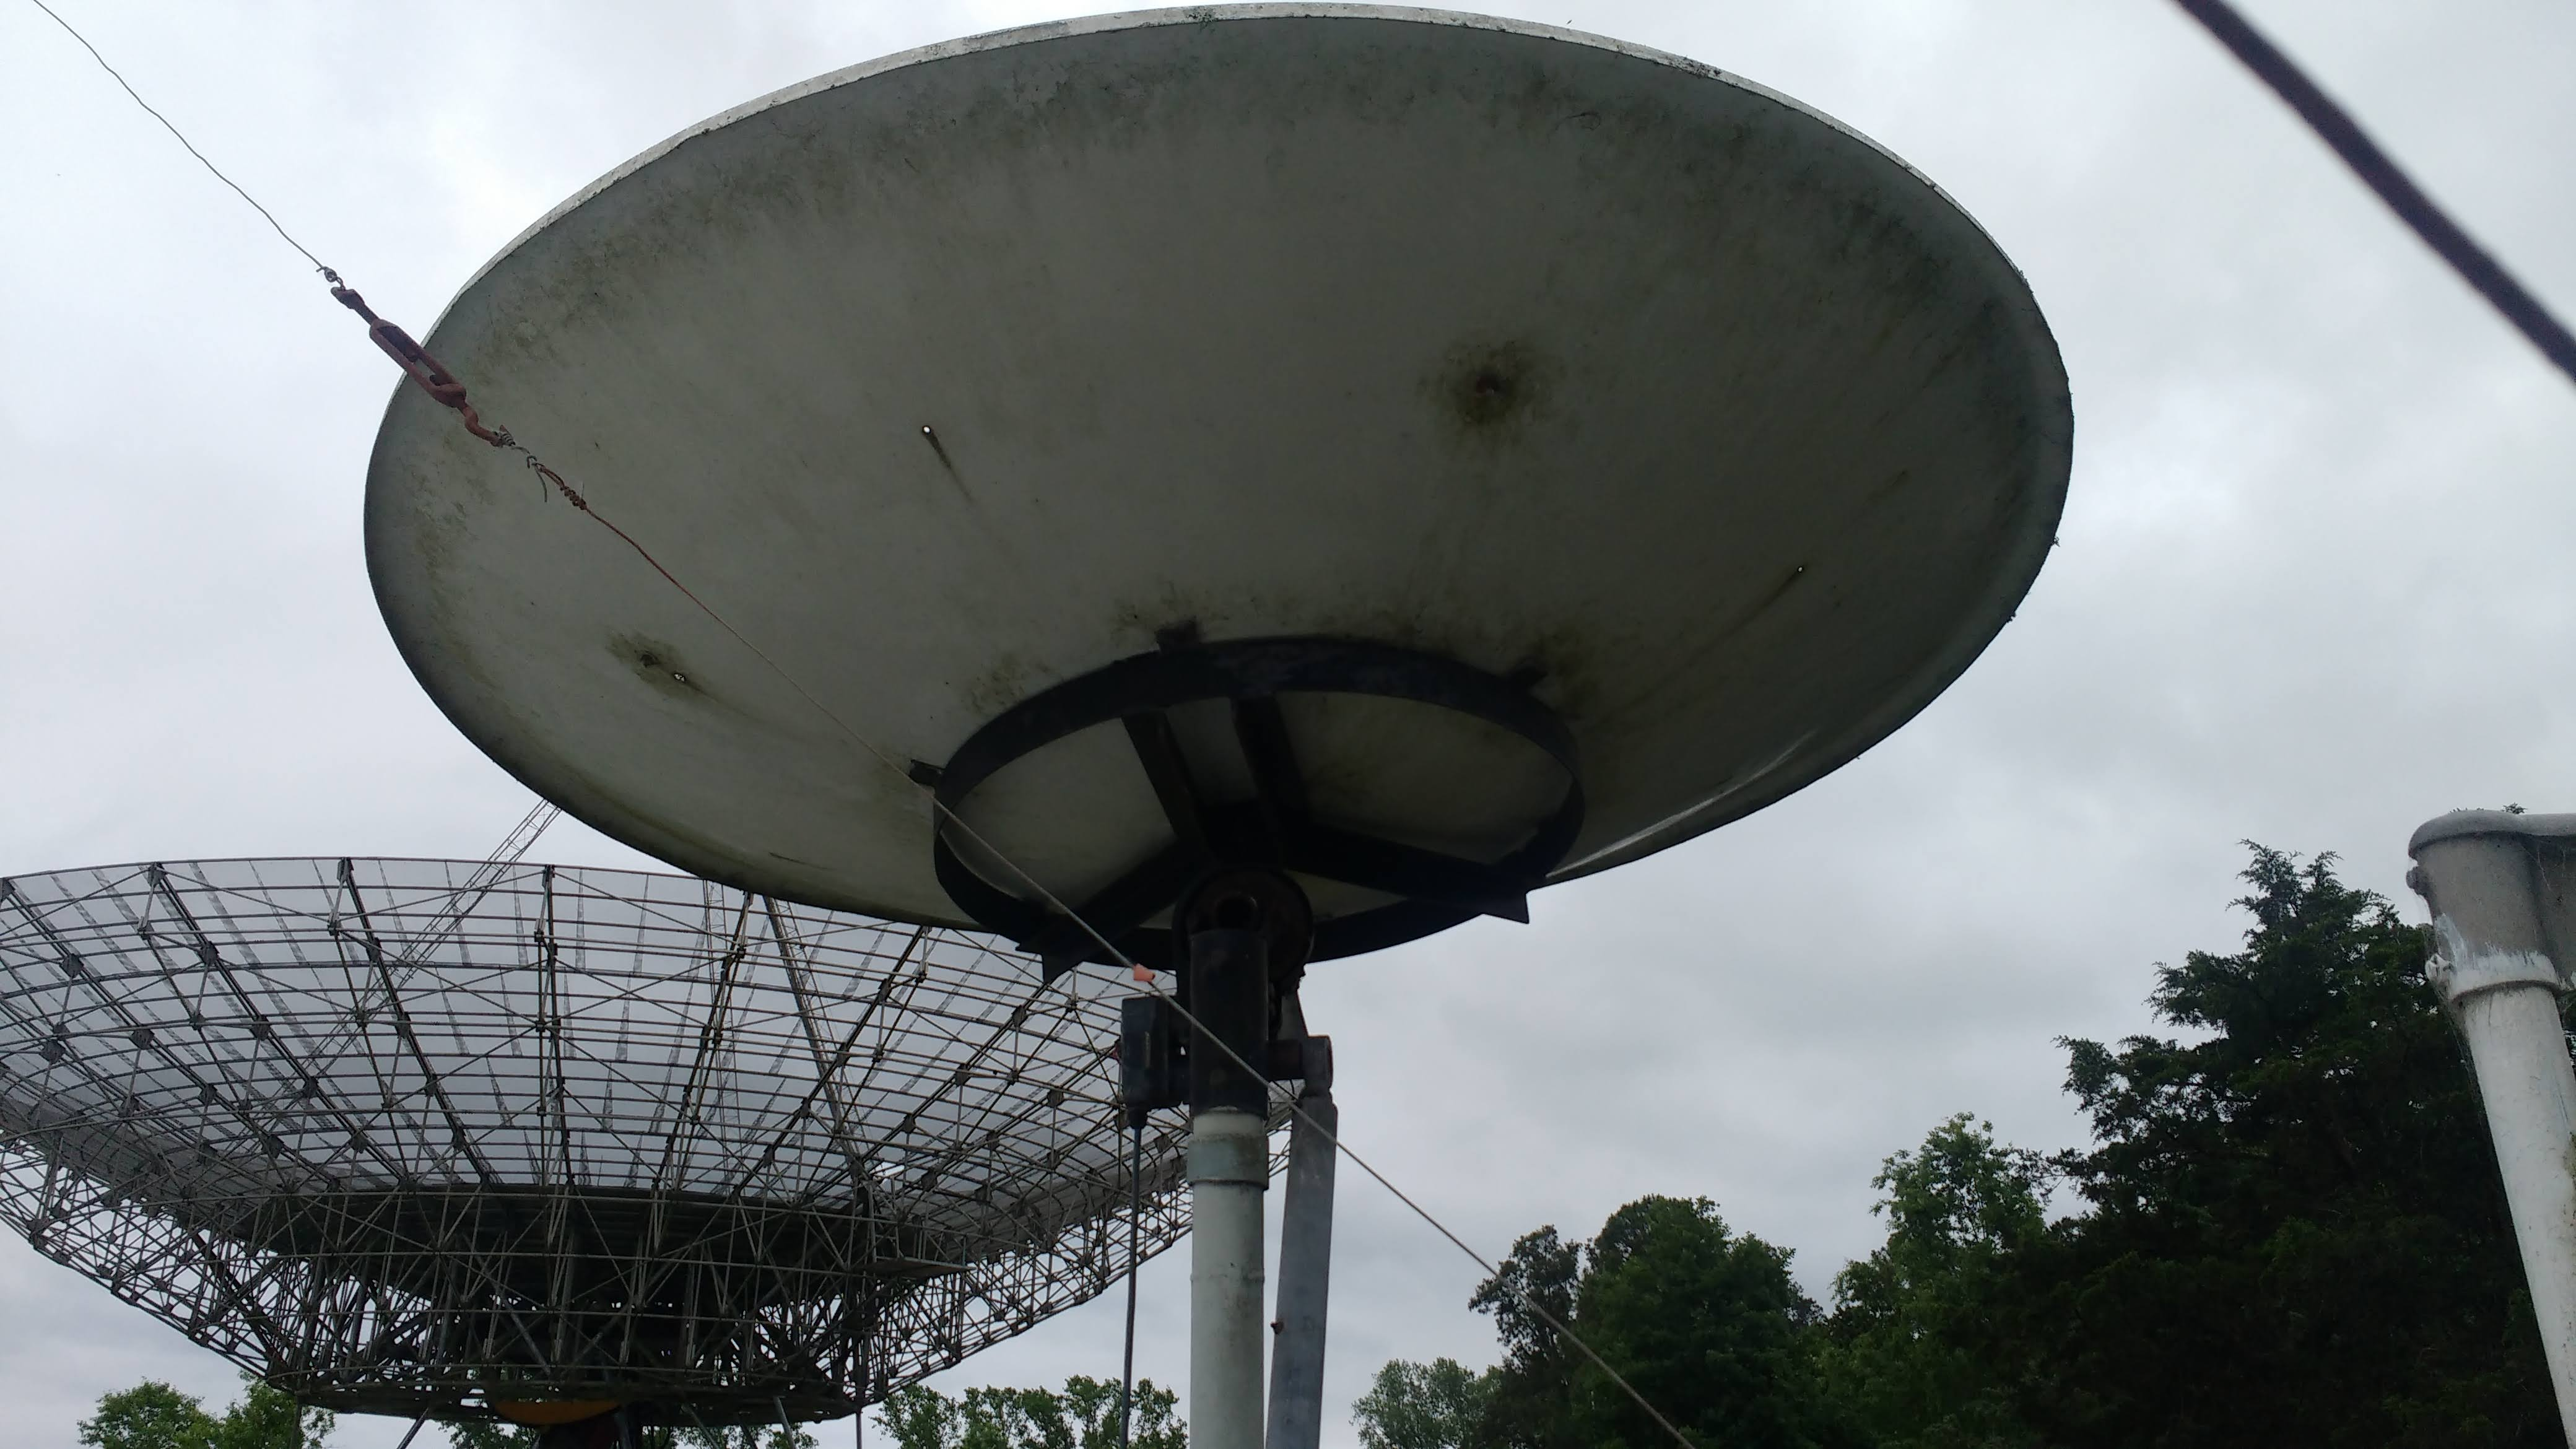
\includegraphics[width=0.5\textwidth]{parte_1/cap1/antena}
	\caption{antena ubicada en el iar, actualmente en desuso}
	\label{fig_antena}
\end{figure}

\section{Descripción de la Antena y posicionador }

La antena tiene el sistema mecánico que se observa en la figura \ref{fig_mec_ant}. 
% iamgen de la mecánica de la antena 
\begin{figure}[ht]
	%\centering 
	\begin{subfigure}{0.5\textwidth}
		\centering
		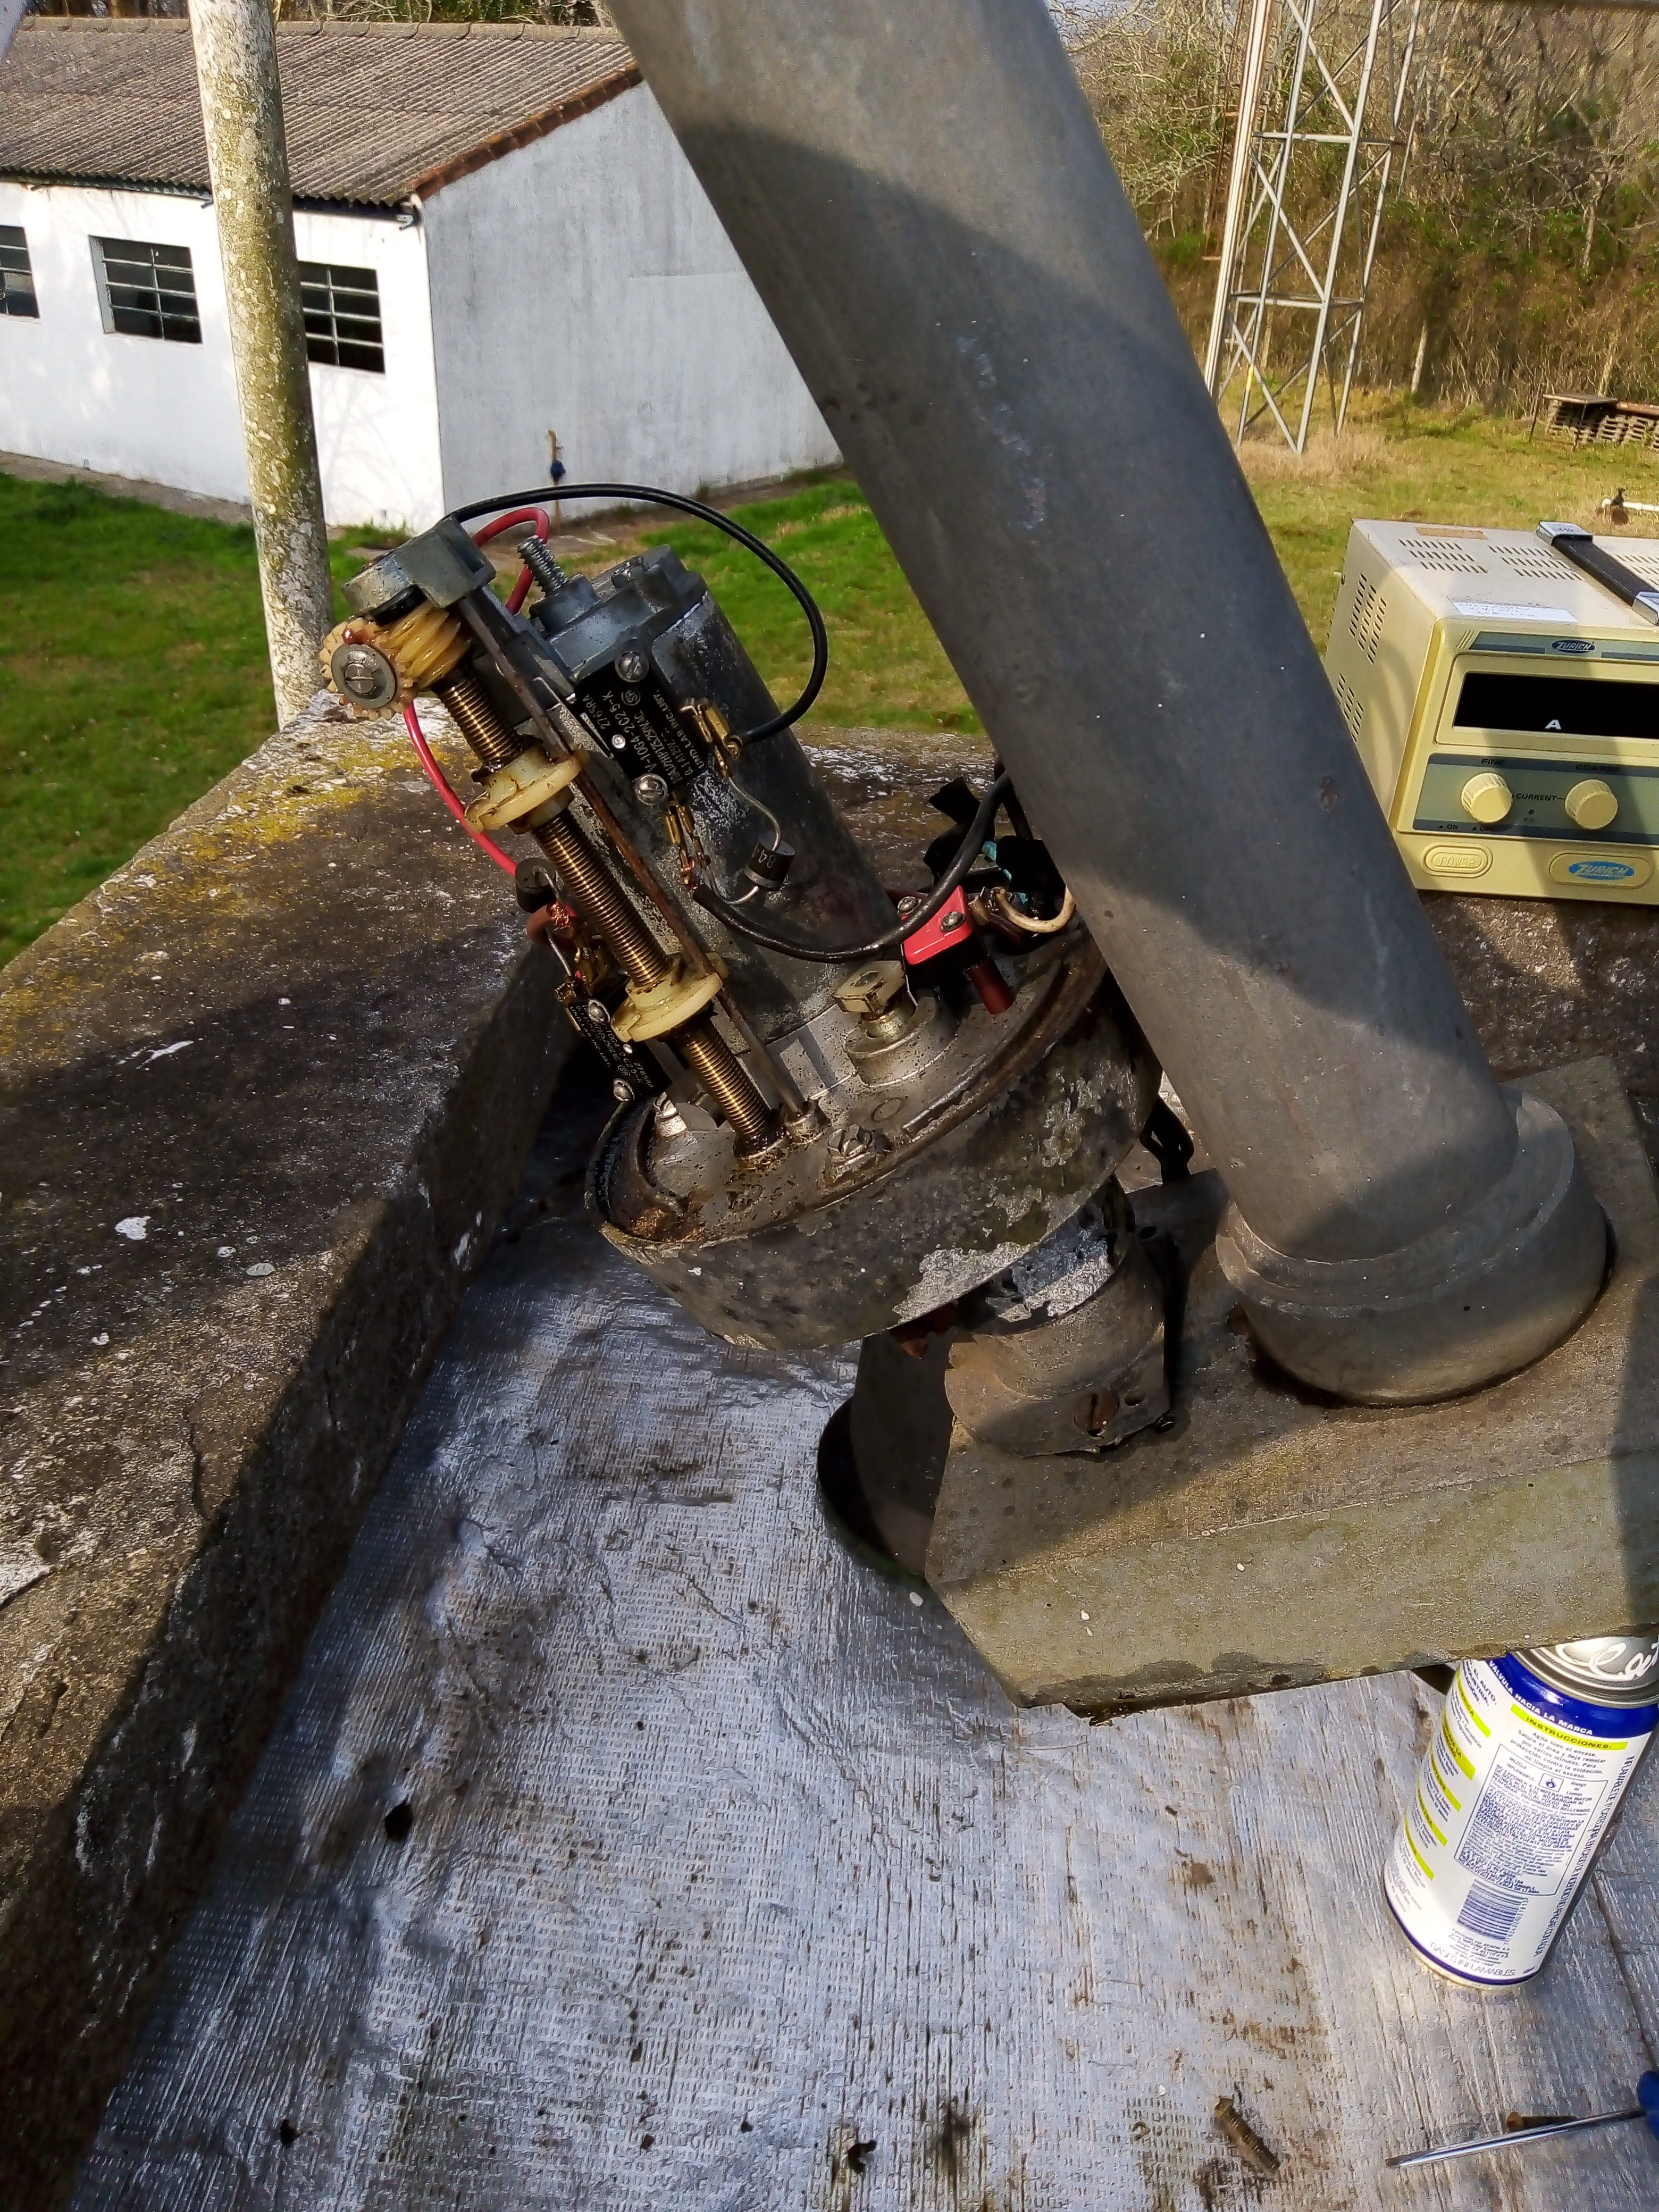
\includegraphics[width=0.5\textwidth]{parte_1/cap1/mot1}
		\caption{Motor del primer eje de la antena }
		\label{fig_mec_ant1}		
	\end{subfigure}
	\hfill 
	\begin{subfigure}{0.5\textwidth}
		\centering
		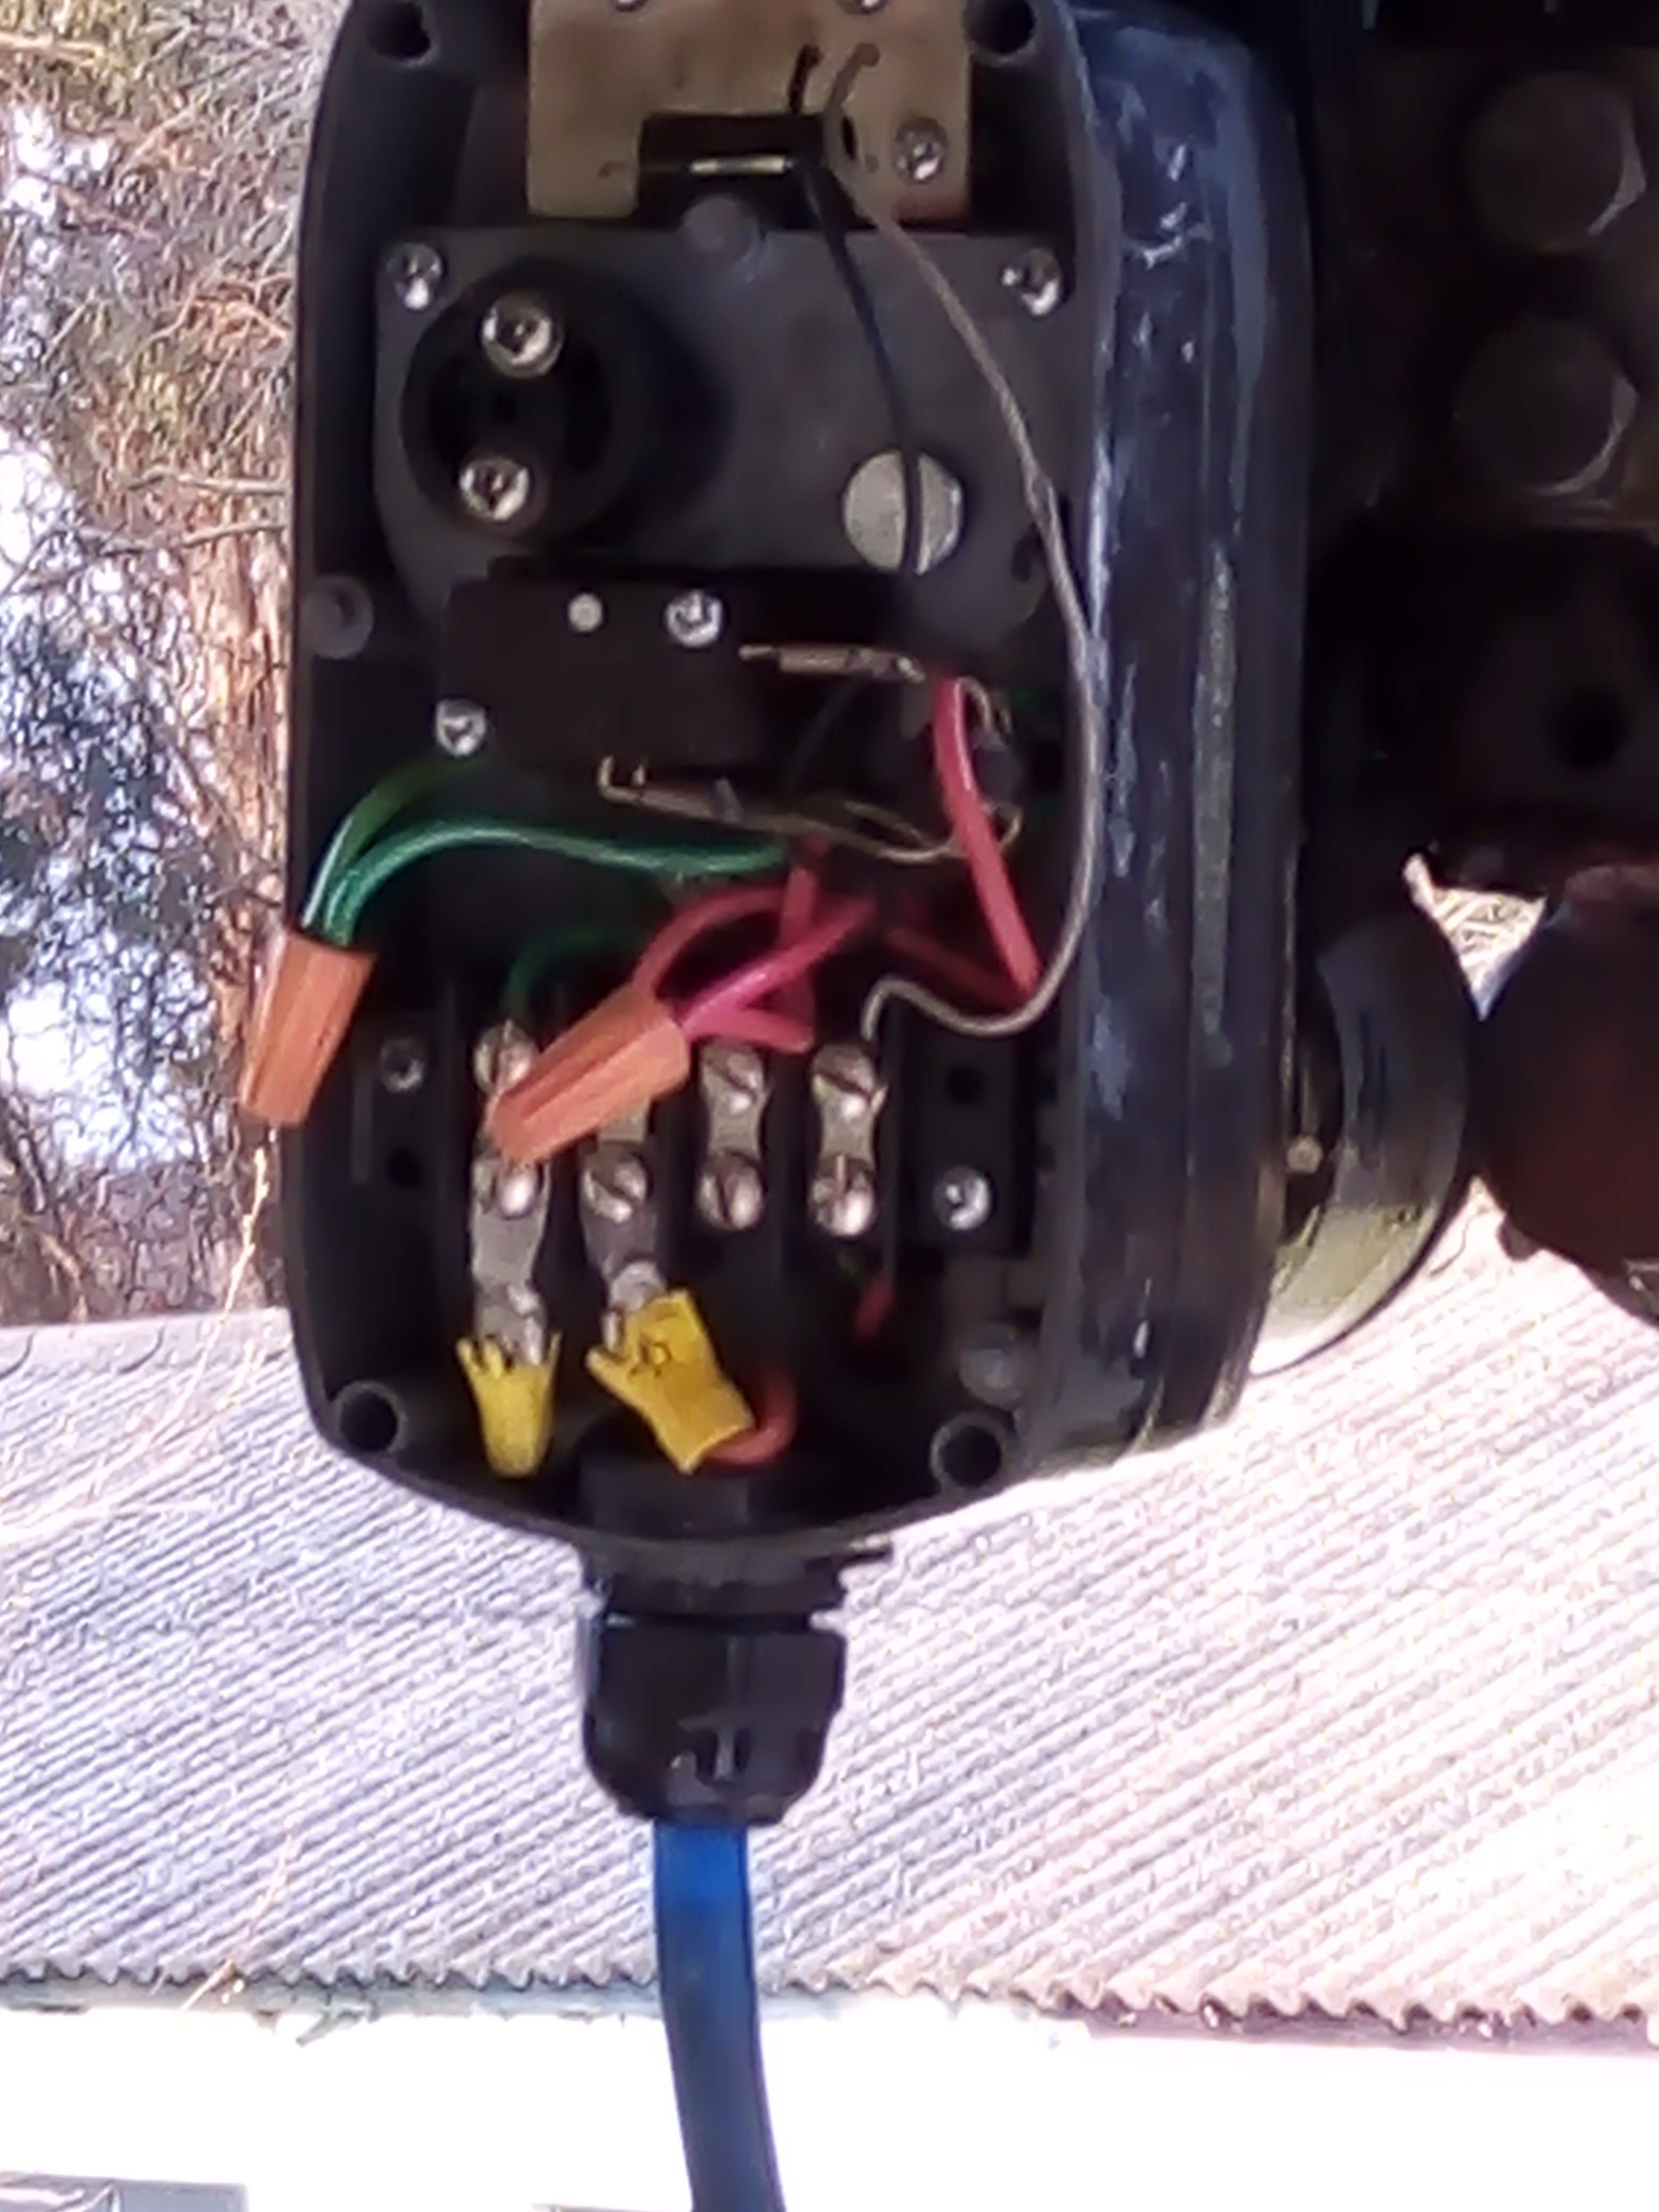
\includegraphics[width=0.5\textwidth]{parte_1/cap1/mot2}
		\caption{Motor del segundo eje de la antena }
		\label{fig_mec_ant2}
	\end{subfigure}
	
	\caption{Encoders asocioados a los motores de las antenas.}
	\label{fig_mec_ant}
\end{figure}


En ella, se observa, que existen dos motores, uno para cada eje, además, tiene un sistema que permite medir la posición de la antena mediante dos potenciómetros adosados al eje de cada motor. Estos ejes son independientes entre sí, y su medida también. 

En el presente trabajo, se va a desarrollar un sistema que sea capaz de realizar el movimiento de la antena, aprovechando el sistema de motores existente sobre la misma. El sistema, que realiza el movimiento de la antena, se conoce como ``posicionador''. Este sistema, recibe una posición, en dos coordenadas, y tiene que mover la antena hacia las coordenadas recibidas. Estas coordenadas que recibe, son las posiciones de los satélites, los cuales se van moviendo, por ende, mientras el satélite este por encima de la antena, o su ``horizonte visible'', debe realizar el seguimiento de la misma, actuando sobre los motores, y acomodando la antena, a donde este el satélite en cuestión.

En la actualidad, existen diversos programas para realizar el seguimiento de satélites en tiempo real, estos consultan bases de datos existentes en Internet, y realizan el cálculo en base a modelos matemáticos. En este documento, se hará uso de alguno de estos programas, para poder actualizar la posición a cada instante y mover los motores hacia donde corresponda. Además, este dispositivo, debe ser controlador desde una PC que esté ubicada dentro de la institución. 

\section{Metodología de trabajo}

El trabajo, se va a dividir en cuatro etapas, denominadas ``fase 1, fase 2, fase 3 y fase 4'' respectivamente. En la primera fase, se va a definir los requerimientos del sistema(capítulo actual), luego se va a proponer una solución a para cumplir estos requerimientos(cap. 2 ), y luego se van a seleccionar algunas piezas electrónicas para la construcción de la solución(cap 3.). 

En la segunda fase, se va a desarrollar el software que debe realizar el sistema de control, tanto para el usuario, como para la computadora que controla la antena. El orden del trabajo, es primero desarrollar el software sobre la computadora, y luego buscar interfaces disponibles, para conectarnos con ese equipo mediante el uso de Internet. 

En la tercera fase, se va a realizar una investigación sobre los sistemas de coordenadas y como se realizan las transformaciones de estas entre sí.

En la cuarta fase, se va a desarrollar el sistema de posicionamiento de los motores, luego se desarrolla la interfaz para conectarse a la computadora que realiza el control del sistema. Luego, una vez desarrollado estas interfaces, se prueba el sistema realizando algún seguimiento, sea a satélites, o a estrellas, o realizando algún apuntamiento de tipo manual. Estas fases, y capítulos a lo largo dle texto, se resumen en la siguiente tabla:    


\renewcommand{\arraystretch}{1.5}

% tabla 
\begin{table}[ht]
	\centering
	\begin{tabular}{|c|c|p{8cm}|}
		\hline
		Fase & Capítulos & Descripción de la fase \\
		\hline 
		\multirow{3}{2cm}{Fase 1} & capítulo 1 & {Definición del proyecto} \\ \cline{2-3}
		& capítulo 2& Definición de los componentes que requiere el proyecto\\ \cline{2-3}
		& capítulo 3& Selección de los componentes de hardware, en base a requerimientos\\ \hline 
%---------------- segunda fase 		
		\multirow{3}{2cm}{Fase 2} & capítulo 4 & Estudio de redes de computadoras \\ \cline{2-3}
		& capítulo 5& Software sobre la PC para el usuario final.\\ \cline{2-3}
		& capítulo 6& Programación del microcontrolador, y conexión con Gpredict y Stellarium\\ \hline 
		

%---------------- tercera fase 		
	   \multirow{2}{2cm}{Fase 3} & capítulo 7 & Sistemas de coordenadas esféricos\\ \cline{2-3}
	   & capítulo 8& Implementación de los sistemas de coordenadas esféricos dentro del microcontrolador.\\ \cline{2-3} \hline 
	   
%---------------- cuarta fase 		
	\multirow{2}{2cm}{Fase 4} & capítulo 9 & Desarrollo de un controlador para los motores de la antena\\ \cline{2-3}
	& capítulo 10& Resultados y conclusiones del trabajo - Futuras versiones\\ \cline{2-3} \hline 
	\end{tabular}
	\caption{Resumen del trabajo en cada fase del proyecto}
\end{table}


\section{ Requerimientos del sistema} \label{req_sist}

De lo expuesto en las secciones anteriores, podemos obtener los requerimientos para este proyecto. Los requerimientos para este proyecto se dividen en dos tipos:  
\begin{enumerate}
	\item Requerimientos Funcionales.  
	\item Requerimientos de sistema. 
\end{enumerate} 
Donde en el primero, se definen aquellas cosas relacionadas al comportamiento del dispositivo a diseñar, mientras el segundo, se refiere a como llevar a cabo la solución en sí. 

%\renewcommand{\multirowsetup}{\centering}

\renewcommand{\arraystretch}{1.5}

\begin{table}[H]
\begin{tabular}{|c|c| p{10cm} | }
% REQUISITOS FUNCIONALES 
	 \hline 	 
	 \multirow{11}{*}[-0.5cm]{\rotatebox[origin=c]{90}{\centering Requerimientos}} 
	 &\multirow{5}{*}[-0.25cm]{\centering Requisitos funcionales} & Medir posición de la antena. \\ \cline{3-3}
	 & & Recibir coordenadas desde una PC dentro del IAR. \\ \cline{3-3}
	 & & Tener control sobre la posición de la antena.\\  \cline{3-3}
	 & & Estacionar la antena en la posición del Cenit cuando no realice seguimientos sobre satélites. \\    \cline{3-3}
	 & & Seguimiento de satélites, naturales y artificiales, y estrellas. \\ \cline{3-3}
	 \cline{2-3}
% REQUISITOS DE SISTEMA 
	 &\multirow{6}{*}[-0.4cm]{\centering Requisitos De Sistema} & No puede utilizar ningún tipo de red inalámbrica. \\ 
	 \cline{3-3}	
	 & & Existencia de componentes en el mercado local. \\
	 \cline{3-3}
	 & & Escalable. \\ \cline{3-3}  
	 & & Independencia entre los componentes del sistema. \\ \cline{3-3}
	 & & Calibración automática del sentido de movimiento y posiciones angulares. \\ \cline{3-3}
	 & & Bajo Costo. \\
	 \hline 
\end{tabular}
\caption{Requerimientos del sistema }
\label{tab:requerimientos}
\end{table}








% imagen de la antena La tabla anterior, nos brinda los requerimientos, sobre los cuales se va a desarrollar el sistema de posicionamiento para la antena en cuestion. Los requerimientos, están de acuerdo, a la necesidad de la institución. 





 

 
%------------Final capitulo 1 ------------------------------%  





\renewcommand{\chaptername}{Componentes para la construcción de posicionador}
\chapter{Componentes para la construcción de posicionador} 
\markright{Componentes para la construcción de posicionador } 
\begin{center}
\begin{tcolorbox}[colback=gray!5!white, %Color del fondo
colframe=gray!75!black,
title= \center{\Large{resumen}} ]
En este capítulo se seleccionan los componentes necesarios para satisfacer los requerimientos de la sección \ref{req_sist}.   
\end{tcolorbox}
\end{center}    
\section{Introducción}

En este capítulo, se muestra que componentes, debe tener el sistema en su versión final. Estos componentes se basan en los requerimientos definidos en la sección \ref{req_sist}. En el mismo, se ha divido en dos tipos de requerimientos: funcionales y de sistema. 

\section{Componentes del Proyecto}

La interconexión de las partes dentro de la institución debe responder al siguiente diagrama del sistema general: 
%---------------- diagrama en bloques -----------------------% 
\begin{figure}[ht]	
	\centering
	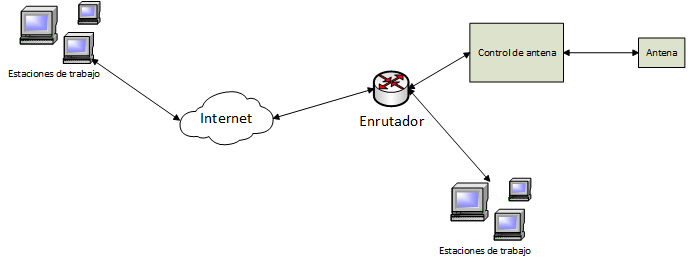
\includegraphics[scale=0.8]{parte_1/cap2/ssgen}
	\caption{Diagrama del sistema general}
	\label{fig:fig_ssgen}
\end{figure}


Donde el bloque desarrollado en la presente tesis es el control de antena de la figura \ref{fig:fig_ssgen},y la configuración de software sobre las estaciones de trabajo dentro de la institución. 

Por lo expuesto en la sección \ref{req_sist}(requisitos del sistema), el sistema que debe realizar el control de la posición sobre la antena debe tener los siguientes componentes: 

\begin{enumerate}
	\item Microcontrolador o computadora para realizar el movimiento de la antena, además debe responder a una PC y comandar el movimiento de la antena.    
	\item Interfaz de usuario con el estado del sistema(interfaz o pantalla para mostrar el estado del sistema).
	\item Interfaz de red, cableada para poder recibir órdenes desde una PC dentro de la institución. 
	\item Mediciones angulares en ambos ejes de la antena.  
	\item Sistemas electrónicos para manejo de motores. 
	\item Software PC de seguimiento de satélites que cuente con conectividad a la red.  
\end{enumerate}

Estos ítems, cumplen todos los requerimientos, tanto funcionales como de sistema. La escalabilidad y la independencia se realiza mediante el microcontrolador, ya qué, se puede actualizar el software sobre el mismo, logrando que el mismo sea escalable. La autocalibración, 
control, y el seguimiento de satélites, naturales o artificiales, y estrellas, se consigue con la combinación del microcontrolador con los sistemas electrónicos de manejo de motores. La recepción desde una PC de los datos, se realiza mediante la interfaz de red. Ambos requerimientos(funcionales y de sistema), deben realizarse mediante la programación del microcontrolador, y la construcción del sistema electrónico de manejo de los motores. Cabe destacar, que se deben realizar dos sistemas electrónicos para el manejo de los motores, ya que el mismo, tiene dos motores, independientes entre sí, el cual genera movimientos independientes de la antena. El requisito de bajo costo y disponibilidad en el mercado local, se analiza en el siguiente capítulo. 


%
%Estas características, para ser cumplidas, requieren que el sistema de control de la antena, tenga una cierta inteligencia para realizar las tareas de manera simultanea. Esto conlleva a que el sistema debe poseer una computadora o microcontrolador capaz de realizar todas estas tareas, además, debe requerir hardware adicional, para interactuar con los motores, y debe requerir algún mecanismo de medición de posición, para poder realizar un lazo de control realimentado. 
%Esto conlleva al siguiente diagrama en bloques, que es el control de antena,de la figura \ref{fig:fig_ssgen} visto con mayor detalles: 
%%\vspace{length}
%
%\begin{figure}[H]
%	\raggedleft
%	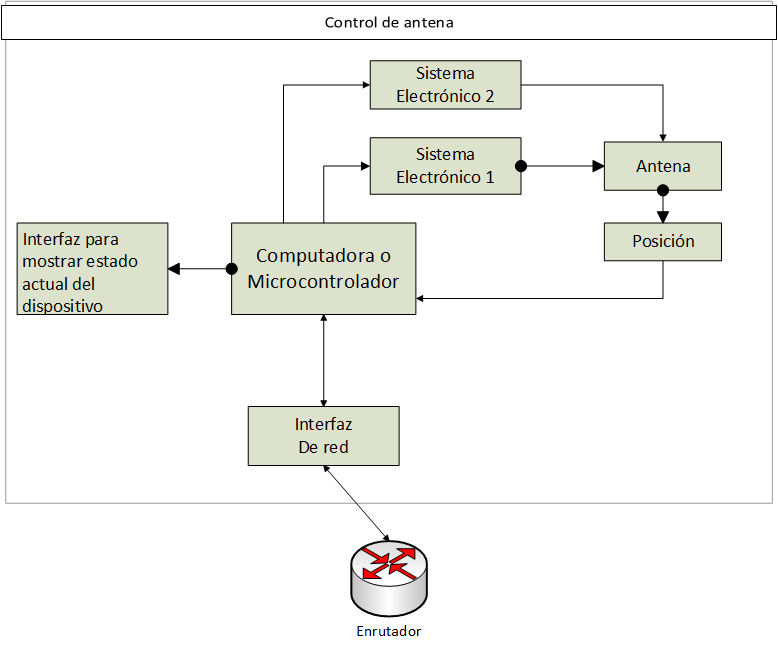
\includegraphics[width= 1.0\textwidth,height=8.6cm]{parte_1/cap2/scontrol} 
%	\vspace{-0.6cm}	
%	\caption{Diagrama del sistema de control}
%	\label{fig_sistema_solucion}
%\end{figure}
%
%En la figura anterior, se tienen dos sistemas electrónicos de posición,ya que la mecánica existente sobre la antena(ver figura \ref{fig_mec_ant} ) permite la independencia de movimientos.  






\renewcommand{\chaptername}{Selección de hardware para implementación del sistema} 
\graphicspath{{parte_1/cap3/}}
\chapter{Selección de hardware para implementación del sistema} \label{cap:cap3_sel_hw}
\markright{\chaptername }
\begin{center}
\begin{tcolorbox}[colback=gray!5!white, %Color del fondo
colframe=blue!75!black,
title= \center{\Large{resumen}} ]
Aquí, definimos algunos de los componentes de hardware seleccionados para cumplir con los requerimientos, en particular, definimos el microcontrolador, la interfaz de red, y la interfaz de usuario del sistema. En esta sección, el análisis se basa sobre componentes disponibles en el IAR, de estos, seleccionamos aquellos, que cumplen el requisito de bajo costo, y luego sobre los mismos, se analiza su facilidad de programación, librerías disponibles, módulos disponibles sobre estos, y otros aspectos.  
\end{tcolorbox}
\end{center}    

\section{Introducción} 
Se definen los criterios de selección del microcontrolador, además, se define la interfaz de red y la de usuario. Los componentes se han seleccionado en base a los siguientes criterios: 
\begin{enumerate}
  \item Compatibilidad entre las partes.  
  \item Disponibilidad de documentación para el desarrollo. 
  \item Cantidad de puertos entrada/salida de cada microcontrolador o computadora 
\end{enumerate}

Al ser una antena, que debe seguir satélites, se debe tener en cuenta, que los satélites, varían su velocidad, según el punto de la órbita en que se encuentren. Dado que esta velocidad varía, este seguimiento, debe adaptarse a estos cambios. Estos cambios son del orden de los segundos, y cualquier microprocesador actual funcionan en orden de los megahertz, con lo cual, si se realiza el control en tiempos del orden de milisegundos, el control podría realizarse sin ningún tipo de inconveniente. Por este motivo, la velocidad de la computadora, no es un factor crítico a tener en cuenta en los puntos de vista para la selección del hardware.    


\section{Componentes de hardware} \label{Sec_CompH}


La computadora, o microcontrolador, debe tener interfaces, para conectarse con el mundo exterior. El hecho es que requiere realizar la medición de dos posiciones en simultaneo, que son el ángulo de acimut y la altura. La antena, posee adosado, dos potenciómetros, que cumplen la función de encoders. Por ende, al tener adosado estos dos potenciómetros, el microcontrolador, debe tener dos canales o puertos de entrada que posean un conversor analógico-digital cada uno. 

La interfaz de red, debe ser independiente del microprocesador o controlador, para cumplir con el requerimiento de escalabilidad, por ende, se debe utilizar alguna solución integrada que se conecte al microcontrolador principal, y puedan intercambiar mensajes entre ellos. 

La interfaz para el estado de la antena, se usará una pantalla, la cual mostrará el estado de la misma. Para ello, se usará un display LCD de 16x2 que se encuentra disponible para su uso.


De lo expuesto en los párrafos anteriores, el microcontrolador, debe ser independiente de todo el hardware asociado. Además debe poseer una electrónica asociada a cada motor, que permita encender o apagar cada motor de forma independiente. Además, debe ser capaz de controlar el sentido de giro de cada motor. Dado que estas maniobras las debe realizar el microcontrolador, se requieren de al menos cuatro puertos disponibles sobre el microcontrolador(dos puertos para cada motor, y con un único puerto, se selecciona el sentido de giro). 


\subsection{Interfaz de red - Materiales disponibles}\label{Int_r} 

La placa disponible en el IAR, es la siguiente: chip Ethernet W5100. Las misma se muestra a continuación. 

\begin{figure}[ht]
	\centering	
	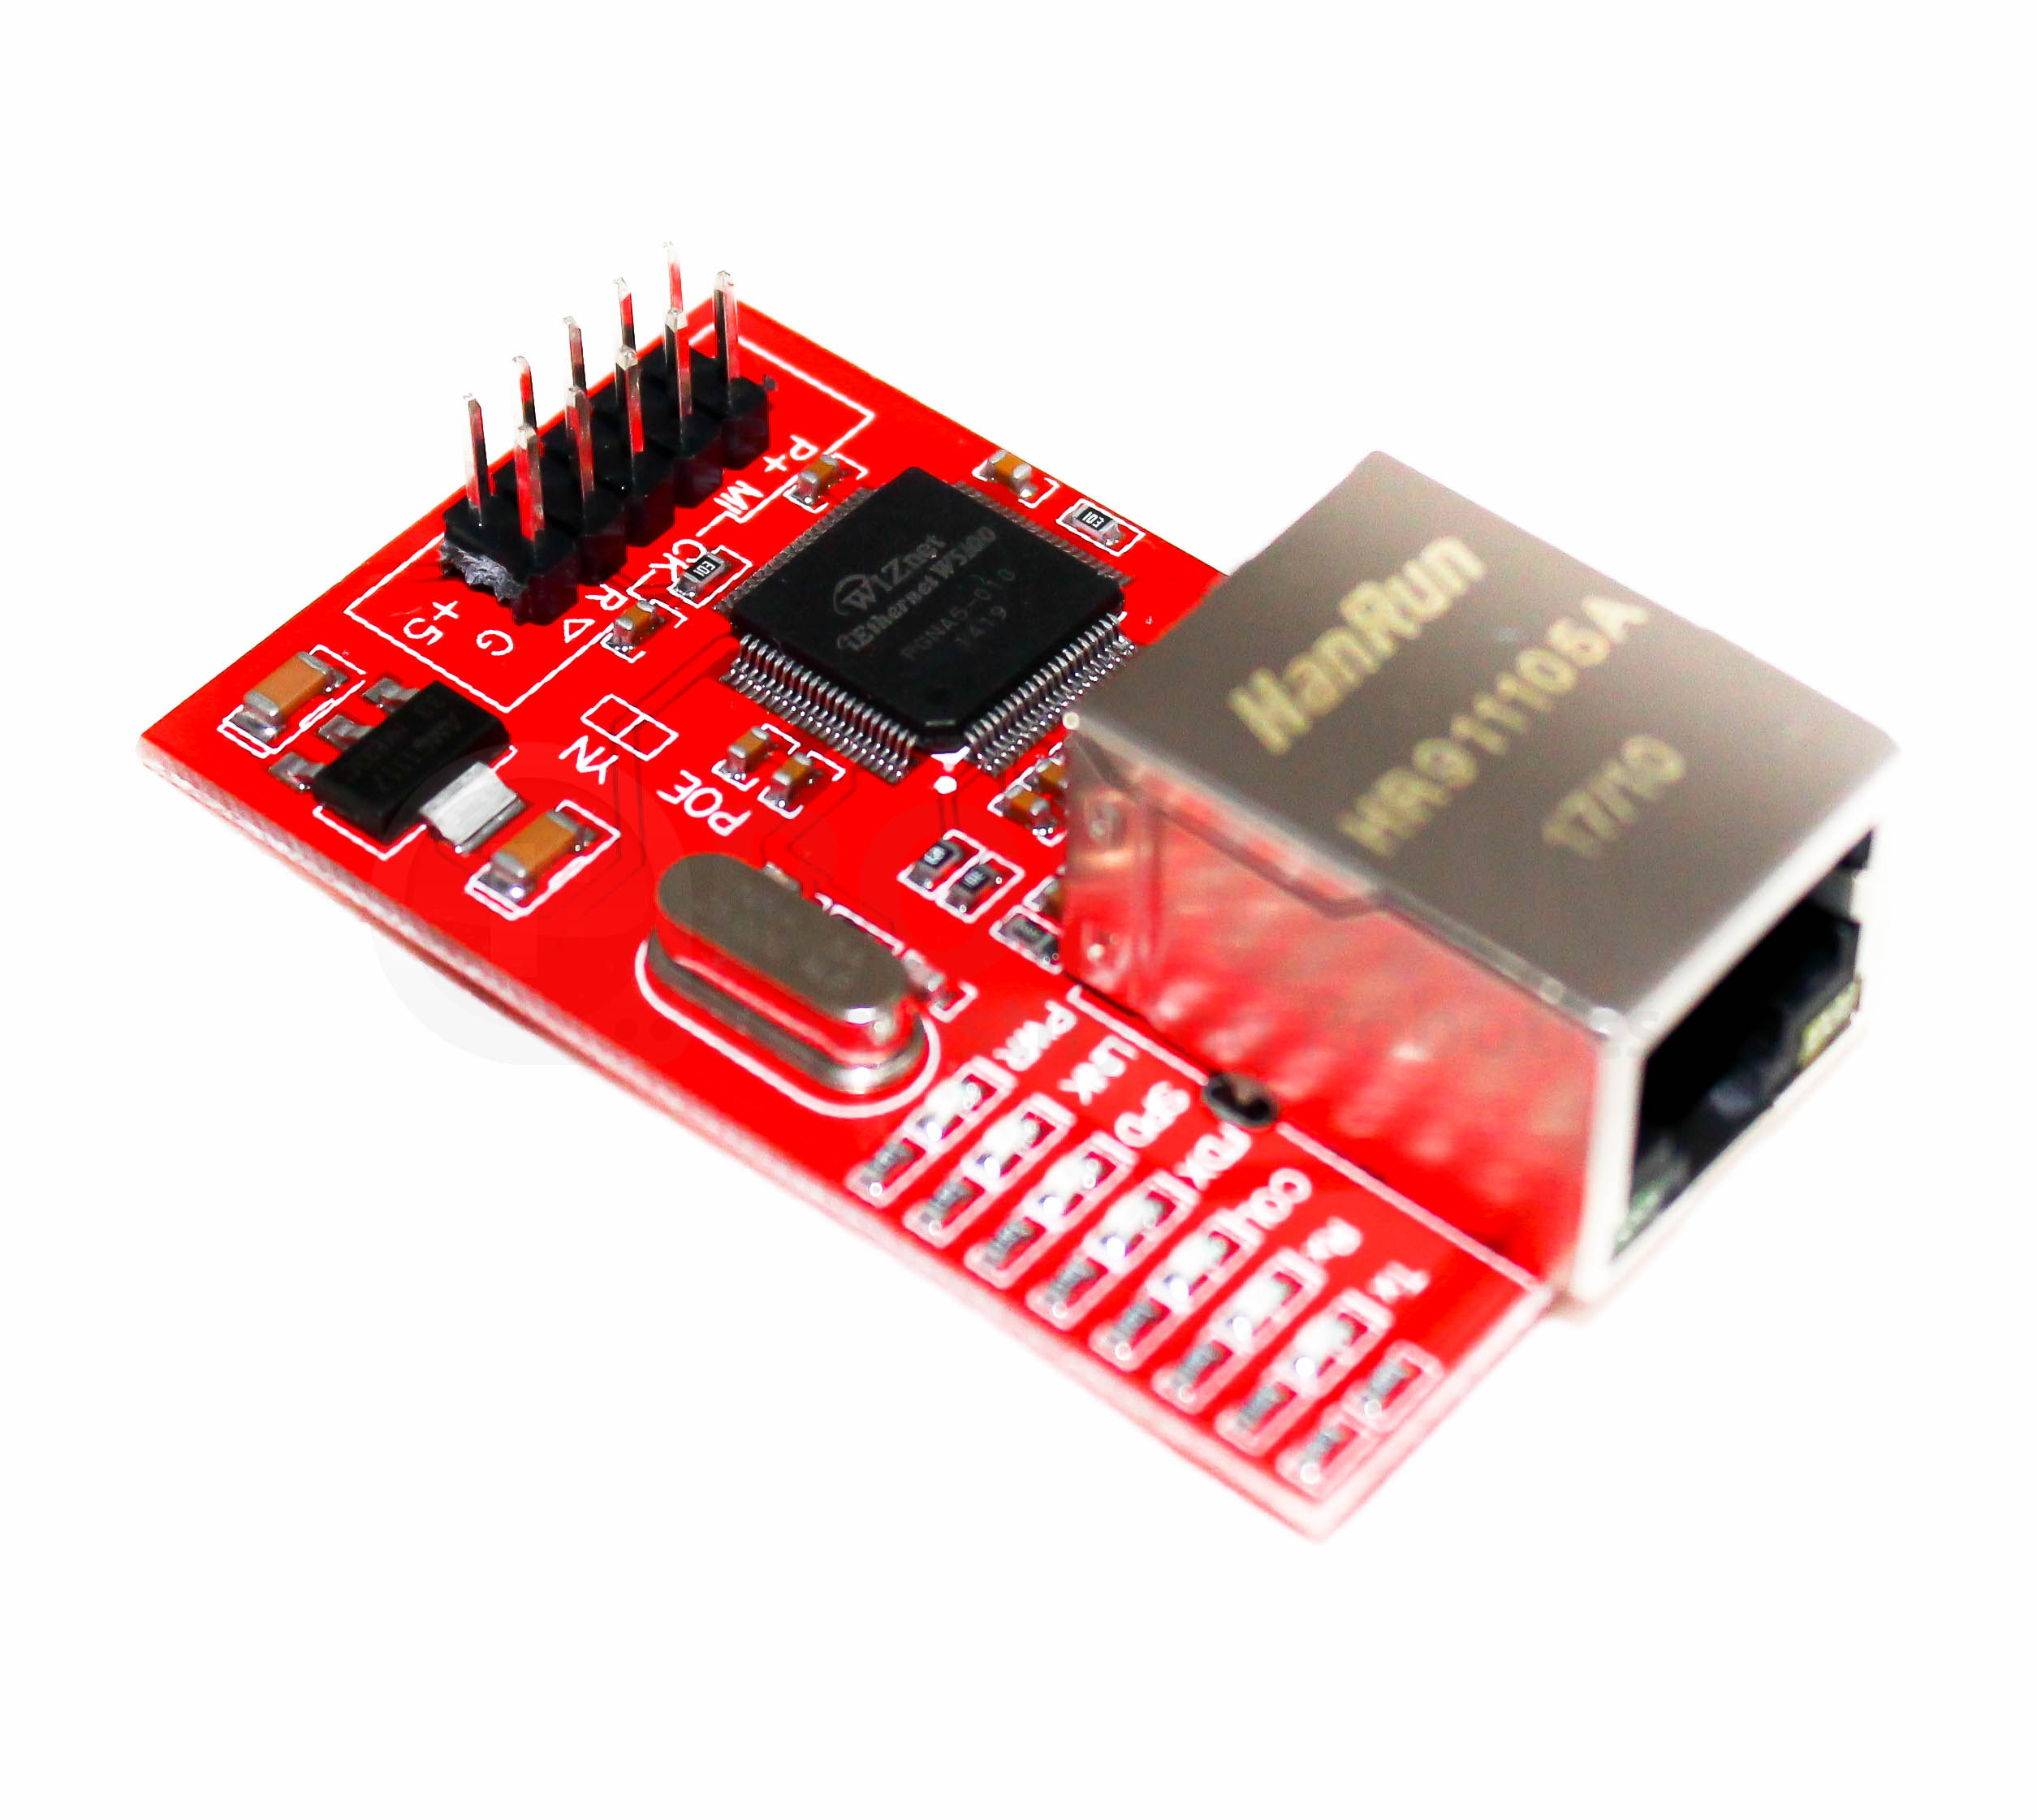
\includegraphics[scale=.2]{w5100}  
	\caption{Chip Ethernet W5100}		 
	%\caption{dispositivos disponibles IAR} 
	\label{fig:chip_ethernet}
\end{figure}

La placa ethernet W5100(ver figura \ref{fig:chip_ethernet}) es un controlador dedicado a las redes. Al recibir un dato, este lo transmite, mediante un puerto paralelo, o por puerto SPI(serial paralell interface). Cabe destacar, que este desarrollo, solo tiene disponible el bus SPI, ya que la placa, solo viene con este protocolo. Además, esta placa, no puede compartir el bus, debido a el diseño de la misma. Si desea compartir el bus, debe modificarse. Uno de los requerimientos es que no debe utilizar redes inalámbricas, por este motivo, se utiliza esta interfaz de red. 

\subsection{Interfaz de usuario} \label{Int_u}
% explicacion display por I2C 
Como se expuso en la sección \ref{Sec_CompH}, se va a utilizar un display LCD de 16 columnas y 2 filas,que está disponible para su uso en el Instituto Argentino de Radioastronomía.  
 
El display LCD, es una pantalla, la cual es capaz de mostrar texto, valores numéricos, crear símbolos propios,etc.El display LCD disponible, se muestra en la figura \ref{fig:LCD_r}: 
\begin{figure}[ht]
	\centering
	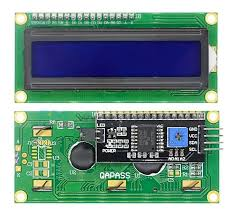
\includegraphics{dispLCD} 
	\caption{Display LCD en el IAR}
	\label{fig:LCD_r}
\end{figure}

La imagen, se ve que el display LCD, tiene adosado, un controlador, este controlador es un circuito integrado denominado PCF8574. Este dispositivo, es capaz, de expandir la cantidad de pines de un microcontrolador, utilizando el protocolo I2C. La ventaja de esto, es que a partir de dos pines se pueden controlar 8 puertos, y esto ahorra en cantidad de puertos de entrada y salida a la hora de elegir el microprocesador. Por ende, el microcontrolador seleccionado debe poseer un controlador o interfaz I2C   



\subsection{Microcontroladores disponibles}  

Los microcontroladores disponibles dentro de la institución, están embebidos dentro de placas de desarrollo, ya diseñadas, y comerciales. Por lo expuesto en las secciones anteriores(ver secciones \ref{Int_r},\ref{Int_u}),el microcontrolador seleccionado debe tener las siguientes características:

\begin{enumerate}
	\item Cantidad de conversores analógico/digital: 2
	\item Cantidad de pines disponibles: 4 (mínimo) 
	\item Puerto SPI: conexionado del chip ethernet
	\item Puerto I2C: para la conexión del display 
\end{enumerate}

 De las placas de desarrollo que hay actualmente en el IAR, se tienen las siguiente placas a analizar: 
 
\begin{enumerate}
	\item EDU-CIAA
	\item Arduino Uno 
	\item STM32VL discovery 
\end{enumerate}
Donde, de las tres, debemos elegir aquella que tenga un menor valor económico, estudiar las soluciones de software y documentación que posean, y revisar si tienen puertos SPI e I2C para el display usado como interfaz de usuario y el chip Ethernet W5100. El estudio realizado se basó en las referencias \cite{placastm32vl,arduno,eduuciaaa}  

% comparación de soluciones: 
\subsubsection{EDU-CIAA}

\begin{wrapfigure}[12]{l}[2mm]{0.4\textwidth}
	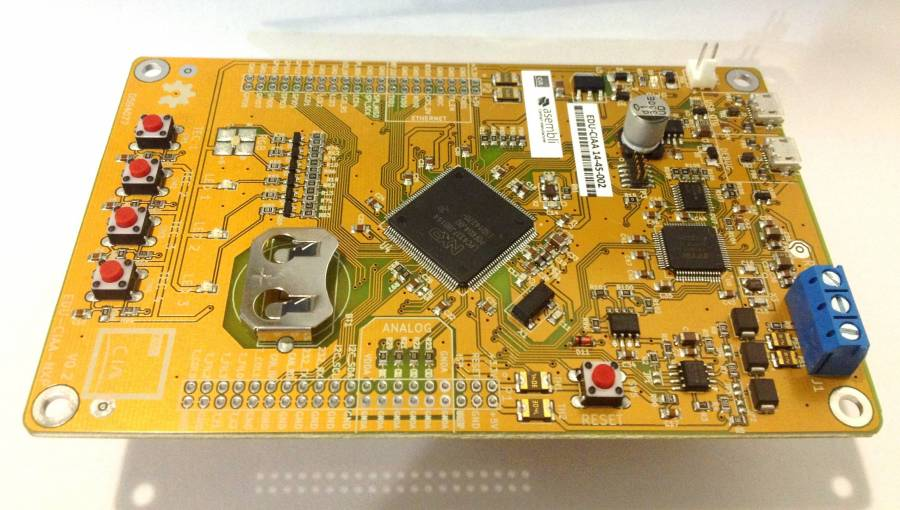
\includegraphics[width=0.4\textwidth , height=  45mm]{edu_ciaa}
	\caption{Eduu Ciaa disponible en el IAR}
	\label{fig:edu_ciaa}
\end{wrapfigure}
La placa EDU-CIAA, es una computadora de software abierto, desarrollada en argentina. Su núcleo se basa en un microprocesador cortex ARM 4.Su microcontrolador es el LPC4337. La documentación existente está incompleta. Algunas partes, están desarrolladas y otras partes, aún están en desarrollo. Posee todas las interfaces necesarias para interactuar con los demás módulos(SPI, I2C,conversores A/D y pines disponibles), se puede realizar una depuración sobre la misma placa,sobre un protocolo denominado JTAG. 


Posee un IDE, y los archivos de compilación(makefile) para cargar el código sobre esta placa. La placa se muestra en la figura \ref{fig:edu_ciaa}. La EDU-CIAA está pensada en software y hardware libre. Todos los esquemáticos de circuitos, y los componentes de software, existen disponibilidad para descargarse y modificarse libremente. 

Esta placa de desarrollo, está pensada para aprender programación sobre microcontroladores, por ende, tiene todas sus interfaces integradas sobre la placa. Posee librerías disponibles para el uso de SPI e I2C. Estas librerías, no poseen documentación, por lo tanto, deben programarse a nivel de registros esta configuración, o realizar una ingeniería inversa sobre las librerías para describir su funcionamiento.    
\vspace{-3mm}
 
\subsubsection{Arduino UNO }
\vspace{-5mm}
\begin{wrapfigure}[11]{l}{0.5\textwidth}
	\caption{Placa Arduino Uno en el IAR}
	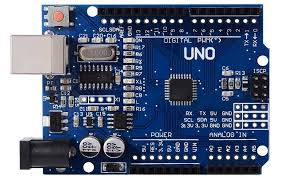
\includegraphics[width=0.4\textwidth , height=  40mm]{arduino_uno}
	\label{fig:arduino_uno}	
\end{wrapfigure}


%\vspace{10mm}
%\hspace{5mm}


La placa de desarrollo, arduino UNO(ver figura \ref{fig:arduino_uno} es una placa de desarrollo basada en hardware y software libre. Está pensada para desarrollos y prototipos rápidos, y posee un entorno de desarrollo integrado, el cual viene preparado para cargar el software dentro de él. Su lenguaje de programación es C/C++. Todos los esquemáticos, y software están disponibles en Internet. Se basa en el microcontrolador AtMega328P.  

Un punto a favor de esta placa de desarrollo, es que poseen librerías para el manejo de los puertos SPI e I2C. En particular, existen librerías para el manejo del display mediante el uso de I2C y el chip ethernet W5100 de manera nativa, es decir, sin necesidad de instalar o descargar ninguna librería adicional. Posee disponibilidad de pines,  y puertos PWM. También posee conversores analógicos digitales. La documentación disponible, se encuentra en su sitio oficial, de manera ordenada. 
La información no oficial, es decir, en Internet es abundante, y existen varios millones de proyectos basados en el ecosistema Arduino dentro de uno de los repositorios más grandes de software: GitHub.    

\subsubsection{STM32VL discovery}
% figura stm32-vl discovery  

\begin{wrapfigure}[12]{l}[10mm]{0.5\textwidth}
	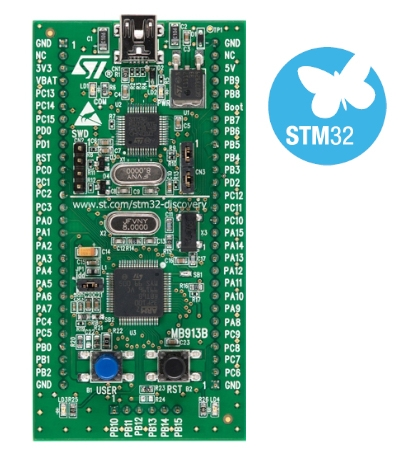
\includegraphics[width=0.4\textwidth,height=45mm] {stm32vl}
	\caption{Placa STM32VLDISCOVERY disponible en el IAR}
	\label{fig:stm32}
\end{wrapfigure}

Esta placa de desarrollo, es desarrollada por la empresa STMicroelectronics. Según la información oficial de su página, esta placa está pensada para el aprendizaje del microcontrolador STM32F100. Este microcontrolador es el núcleo de esta placa,es un procesador con arquitectura ARM. Tiene 64 pines disponibles, varios conversores analógicos digitales. Tiene ejemplos y disponibilidad de software en forma gratuita. No posee documentación sobre la construcción de la placa. Existe muy poca información por fuera de la documentación oficial. Existen algunos foros de sistemas embebidos, pero la discusión es muy escasa, y en general se encuentra en idioma inglés. La placa se muestra en la figura \ref{fig:stm32}




\subsubsection{Comparación de microcontroladores} 
Dado, que se han analizado las tres placas de desarrollo que están disponibles, se van a comparar sus prestaciones y además su disponibilidad en el mercado local. Esto se realiza, basado en las hojas de datos de cada microcontrolador. Este es necesario, ya qué si el equipo se daña durante el desarrollo, o mediante su uso, puede cambiarse de forma inmediata, sin pérdida de tiempo. Esta comparación se realiza en la siguiente tabla:  

% tabla comparativa 
\renewcommand{\arraystretch}{1.2}
\begin{table}[ht]
\makebox[15cm][c]{
\begin{tabular}{|l|c|c|c|}
	\hline
	\textbf{Nombre de la placa} & Arduino Uno & EDU-CIAA &STM32VLDISCOVERY \\
	\hline 
	\textbf{Microcontrolador} & ATmega328P & ARM Cortex-M4F & STM32F100 \\
	\hline 
	\textbf{Canales ADC} &6 canales -10 bit & 3 canales -10 bit  & 16 canales - 12bit \\ 
	\hline 
	\textbf{Puertos Disponibles } & 15 & 80 & 70 \\ 
	\hline 
	\textbf{Comunicación I2C} & Si & Si &Si \\
	\hline 
	\textbf{Comunicación SPI}  & Si & Si &Si \\ 
	\hline 
	\textbf{Disponibilidad} & Si & No  &No  \\
	\hline 
	\textbf{Precios promedios} & \$1000(disponible en todo el país) &\$5.732({único local})  & \$5100(mercado limitado)  \\ \hline
\end{tabular}
}
\caption{Cuadro comparativo de placas disponibles en el Instituto Argentino de radioastronomía}
\label{tab:comp_mc}
\end{table} 




% Explicar muy bien porque se selecciono el microcontrolador

De la tabla \ref{tab:comp_mc}, la placa seleccionada es la denominada Arduino UNO, ya que posee soluciones de software sobre el display, y soporta el chip ethernet W5100 de manera nativa. Esto, implica que la velocidad de desarrollo es superior a la de las otras placas, ya que no se requieren conocimientos detallados sobre los protocolos. 

Por último, el hardware seleccionado para realizar la segunda fase de esta tesis es el siguiente: 
\begin{enumerate}
	\item Placa de desarrollo o microcontrolador: Arduino UNO 
	\item Interfaz de red: Chip Ethernet W5100 
	\item Interfaz de usuario: Display LCD  
\end{enumerate}

Estos tres componentes, ante cualquier tipo de falla, están disponibles en el mercado local, y esto facilita el seguimiento del proyecto en caso de algún fallo en los componentes de hardware. 



%-----------------fin primera fase --------------%

%-----------------segunda fase ------------------%
\part{ Desarrollo de software y redes TCP/IP, Interfaz PC- usuario }


\renewcommand{\chaptername}{Redes}  
\graphicspath{{parte_2/redes/}}
\chapter{Redes}
\markright{\chaptername }

% resumen del capitulo 
\begin{center}
	\begin{tcolorbox}[colback=gray!5!white, %Color del fondo
		colframe=blue!75!black,
		title= \center{\Large{resumen}} ]
		Se definen los componentes básicos de una red: los modelos OSI y TCP/IP. Luego analizamos los protocolos TCP, y DHCP,y el protocolo IP. Luego, se propone el software WireShark para ver estos protocolos funcionando sobre una red ya implementada. 

	\end{tcolorbox}
\end{center}    
\section{Introducción} 
En este capítulo analizamos las redes de computadoras,y como se conectan entre sí los dispositivos de una red. Ademas, se analizan dos modelos de capas principales: OSI y TCP/IP, donde cada uno consta de varias capas, donde se brinda un breve resumen de cada capa. 
Luego, se analizan, dos protocolos para reconocer dispositivos en una red, el protocolo DHCP,que le asigna una dirección, y el protocolo IP,que le asigna una red. Además, se introduce el concepto de sniffer, y se muestra como visualizar el contenido de los datos que están circulando en una red. Los conceptos en que profundiza el presente capítulo, son aquellos de mayor interés para la construcción del dispositivo.  


\section{Redes de Área local }
Existen tres tipos de redes: Redes de área local, de área metropolitana, y redes de área amplia. El dispositivo desarrollado en el presente trabajo, se conecta a la red de área local de la institución, por ende, es importante entender de una manera elemental el funcionamiento de las redes, sus protocolos, y sus modelos de capas.   

Las redes de área local, son aquellas que se interconectan distintos equipos de una institución, departamento de una empresa, etc, para que se realice un intercambio de información, a través de un medio. Las redes de área local, generalmente se dice que son redes LAN, por sus siglas en inglés(Local Area Network).  En general, son redes de propiedad privada. Existe un estándar, para estas redes LAN cuando se conectan de forma inalámbrica: IEEE 802.11 (comúnmente denominado WiFi), y cuando son alámbricas existe el estandar IEEE 802.7(comúnmente denominado ethernet). Las redes WiFi, no se utilizan en este trabajo, por utilizar técnicas de radiofrecuencia, que interfieren con los receptores de comunicaciones.  
En el caso de redes alámbricas, las computadoras, realizan un enlace punto a punto, a través de un dispositivo denominado \textbf{Switch}.Un switch, posee varias entradas para conectar mas de una PC,y el trabajo de este, es transmitir mensajes entre computadoras, conociendo la dirección de destino, que viene incluida en el mensaje. Si se requieren redes mas grandes, pueden interconectarse Switchs entre sí, y armar redes de mayor tamaño. 


En el presente trabajo, se conecta el dispositivo a un switch, que esta ubicado en sala de control,del Instituto Argentino De Radioastronomía. Ademas al finalizar el trabajo, se solicitará que se le asigne una dirección fija dentro de la red institucional.  

En el trabajo realizado en este presente informe, usamos un modelo conocido como arquitectura "cliente-servidor". Esta arquitectura, se basa en que hay maquinas clientes, que solicitan un servicio, a otra estación de trabajo, denominada servidor. Los clientes, son las estaciones de trabajo del lugar, y el servidor es el dispositivo desarrollado en esta tesis, ya que es el qué brinda el servicio de apuntamiento de antena. En otras palabras, las estaciones de trabajo deben conectarse al dispositivo desarrollado en el presente documento. De ahí, que se requiera el permiso correspondiente para fijar la dirección del dispositivo.  




\section{Modelo de capas}

para reducir la complejidad de las redes, se organizan en capas, donde cada capa, ofrece ciertos servicios a capas superiores, mientras les oculta detalles relacionados con la forma en que se implementan estos servicios. El uso de capas, no es un problema inherente de las redes, sino que se aplica en otros ámbitos de las ciencias de la computación. La cantidad de capas es variable, y depende del problema en cuestión. En términos de redes de computadoras, se usan dos modelos principalmente, el modelo OSI y el modelo TCP/IP. El primero consta de siete capas, el segundo consta de cinco capas. 

para entender este sistema de capas, consideramos una capa y le ponemos un numero K. Supongamos que la capa K de una PC desea comunicarse con la capa K de otra. La forma en que ambas se comunican, se denomina protocolo, que define las reglas y convenciones usadas en esta comunicación. 

\begin{wrapfigure}[21]{l}{0.4\textwidth}
	\centering 
%	\caption{Conexion entre capas.En esta figura se observan la interface,protocolo y conexionado}
	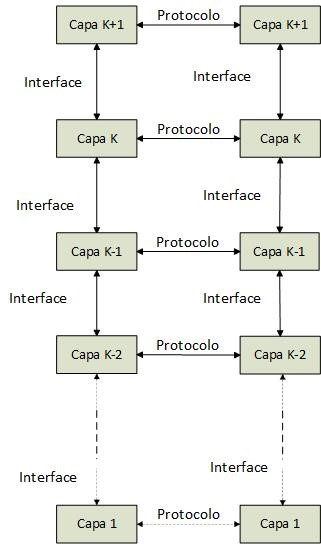
\includegraphics[scale=0.6]{modcap}
	\caption{Conexión entre capas.En esta figura se observan las interfaces,protocolo y conexionado}
	\label{fig:modOSI}	
\end{wrapfigure}
En realidad, las capas, no se comunican directamente entre sí, sino que pasan la información (datos y control) a la capa inferior (en nuestro ejemplo, capa k-1), y así, hasta el nivel mas bajo (capa 1). En el nivel mas bajo, envía la información a otra maquina dentro de la red, y ella se encarga de pasar los datos a las capas superiores, en un proceso inverso al realizado para enviar la información. La comunicación entre capas se realiza a través de una entidad denominada interface. La figura  \ref{fig:modOSI} ilustra el proceso de capas descrito.

A un conjunto de capas y protocolos se conoce como Arquitectura de Red. La especificación de una arquitectura debe contener suficiente información como para permitir que un programador escriba el programa, o construya el hardware para cada capa, de manera que se cumpla correctamente el protocolo apropiado.

Debido a que existen muchas computadoras dentro de una organización, estos protocolos, necesitan de alguna manera identificar el destinatario del mensaje y quien lo envía, esto se denomina direccionamiento o nombramiento en las capas. para realizar esto, se definen dos modelos: El modelo OSI y el modelo TCP/IP. Se diferencian en la cantidad de capas de cada modelo, los nombres de cada capa, pero la funcionalidad sigue siendo la misma: intercambiar información entre dos dispositivos, usando un esquema de capas, las cuales permiten que el diseñador tenga mas facilidad a la hora de diseñar una red. 



\subsection{Modelo OSI}
El modelo OSI, se basa en una propuesta desarrollada por la organización internacional de normas(ISO), en un intento de estandarización para los protocolos. En si, es un modelo general, pero sus protocolos no se utilizan masivamente.La sigla OSI proviene de ''open system interconection''(sistema de interconexión abierto). Este modelo tiene siete capas, y los principios utilizados para llegar a ellas son los siguientes:
\begin{enumerate}
	\item Se debe crear una capa en donde se requiera un nivel diferente de abstracción 
	\item Cada capa debe realizar una función bien definida 
	\item La función de cada capa se debe elegir teniendo en cuenta la definición de protocolos estandarizados
	internacionalmente
	\item Es necesario elegir los límites de las capas de modo que se minimice el flujo de información a través de las interfaces 
	\item La cantidad de capas debe ser suficiente como para no tener que agrupar funciones distintas en
	la misma capa; ademas, debe ser lo bastante pequeña como para que la arquitectura no se vuelva
	inmanejable. 
\end{enumerate} 
Las capas, se muestran en la figura a continuación:% \ref{fig:mod_osi}:
\vspace{-2mm}  
\begin{figure}[ht]
	\centering
	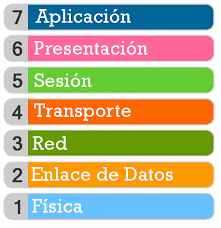
\includegraphics[scale=0.5]{modelosi} 
	\caption{Capas del Modelo OSI}
	\label{fig:mod_osi}
\end{figure}  


\subsubsection{capa 1 - Capa física} 
Esta capa, se relaciona con la transmisión de bits a través de un canal de comunicación. Los aspectos de diseño tienen que ver con las interfaces mecánica, eléctrica y de temporización, así como con el medio de transmisión físico que se encuentra bajo la capa física.


\subsubsection{capa 2 - Enlace de datos } 
La función principal es transformar un medio de transmisión puro, en una linea que esté libre de errores. Ademas, proporciona medios para activar,desactivar y mantener el enlace(es decir, la comunicación). Aquí, esta definido un componente de hardware: la tarjeta o placa de red. Cada placa de red tiene un número único conocido como MAC address, y es único para cada dispositivo en el mundo. 

\subsubsection{capa 3 - Capa de red}
La capa de red, realiza la transferencia de información entre sistemas finales, liberando a las capas superiores del conocimiento de los medios de transmisión y tecnologías de conmutación usadas. 

Si hay demasiados paquetes en la subred al mismo tiempo, se interpondrán en el camino unos con
otros y formarán cuellos de botella. El manejo de la congestión también es responsabilidad de la capa de
red, en conjunto con las capas superiores que adaptan la carga que colocan en la red.
\subsubsection{capa 4 - Transporte }
En esta capa, se reciben datos de las capas superiores, y los '' particiona'' en unidades mas pequeñas, para ser enviadas a las capa de red.Ademas,debe asegurarse  que estos paquetes lleguen a destino. En otras palabras, parte los mensajes de las capas superiores para ser transmitidas al medio de comunicación. 

\subsubsection{capa 5 - Sesión  }
Esta capa, proporciona mecanismos para el control del diálogo (decidir quien debe transmitir)entre las aplicaciones de los sistemas finales. En muchos casos, estos servicios son totalmente  imprescindibles,sin embargo, en algunas aplicaciones, su utilización es obligatoria. 

\subsubsection{capa 6 - Presentación}
Aquí, se define el formato de los datos que van a intercambiarse en las aplicaciones., y ofrece a las aplicaciones un conjunto de servicios de transformación de datos. Ejemplos específicos, son compresión y cifrado de datos. 


\subsubsection{capa 7 - Aplicación} 
Esta capa, proporciona a los programas de aplicación, un medio para que accedan al entorno OSI. Aquí, se encuentran funciones de administración, y los mecanismos para la implementación de aplicaciones distribuidas. En esta capa, tenemos las aplicaciones de uso general, como la transferencia de ficheros, correo electrónico, navegadores web,etc. 


\section{Modelo TCP/IP} 
  El modelo TCP/IP es usado para conectar computadoras entre si a través de una red interna dentro de una organización. Este modelo se muestra en la figura \ref{fig:model_tcpip}, y se dará una breve explicación de cada capa: 
  \begin{figure}[ht]
  	\centering
  	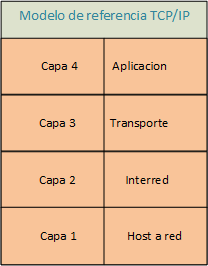
\includegraphics{model_tcpip}
  	\caption{Modelo de capas TCP/IP}
  	\label{fig:model_tcpip}
  \end{figure} 

\subsection{capa 1 - Capa de Host a red}
La capa 1,del modelo TCP/IP, también se la suele nombrar capa de enlace.En este documento utilizamos como nombre de capa ''host a red''.De esta capa, no se puede decir mucho, excepto que puntualiza que el host se debe conectar a la red mediante el mismo protocolo para que se puedan enviar paquetes IP (véase la siguiente sección). Este protocolo no está definido y varia de una red a otra.
\subsection{capa 2 - Interred}
Su trabajo es permitir que los hosts inyecten paquetes dentro de cualquier red y que viajen a su destino de manera independiente. Una analogía es el servicio de correo. Una persona, deposita una serie de cartas internacionales en un buzón, y la mayoría de ellas se entregarán en la dirección correcta del país de destino. Es probable que las cartas, viajes a través de una o mas puertas de enlace de correo internacional, pero esto es transparente a los usuarios. Este trabajo, lo realiza la capa de interred, que da transparencia a los usuarios de como viajan estos paquetes dentro de una red. 
La capa de interred, define un paquete de formato y protocolo denominado protocolo IP (Internet protocol). El trabajo de la capa de interred es entregar paquetes IP al destinatario. 

\subsection{capa 3 - Transporte}
Está diseñada para permitir que las entidades iguales en los hosts origen y destino puedan llevar a cabo una conversación. Aquí se han definido dos protocolos de transporte de extremo a extremo: el TCP (protocolo de control de transmisión), es un protocolo confiable, que permite un flujo de bytes que se origina en una máquina se entregue sin errores en cualquier otra máquina. Divide le flujo de bytes entrantes en mensajes discretos y pasa cada uno de ellos a la capa de interred. En el destino, ocurre el proceso inverso, es decir, el destino reconstruye el mensaje recibido. TCP maneja control de flujo para asegurarse que un emisor rápido no sature a un receptor lento con mas mensajes de los que puede manejar. 
El segundo protocolo de esta capa UDP (protocolo de datagrama de usuario) es un protocolo no confiable, se usa para aplicaciones que no desean la secuenciación o control de flujo de TCP y desean proporcionar el suyo. Es decir, se usa en aplicaciones donde la entrega puntual es mas importante que la precisa. 



\subsection{capa 4 - Aplicación}
Contiene todos los protocolos de nivel mas alto. Los primeros fueron TELNET, FTP, SMTP, etc. Con el tiempo, se han agregado otros protocolos, por ejemplo, HTTP, DNS, etc. 
En la siguiente imagen, se muestra la relación entre las capas del modelo TCP/IP
%\vspace{-1cm}
\begin{figure}[ht]
	\centering
	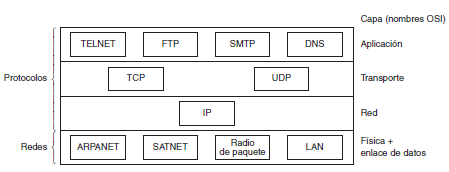
\includegraphics[height=5.0cm]{cap_ap_tcpip}
	\caption{Esquema de interconexión del modelo TCP/IP}
\end{figure}


\section{OSI vs TCP/IP }

Los dos modelos tienen mucho en común. Ambos se basan en un modelo de capas, independientes entre sí. Es importante tener en cuenta que se están comparando los modelos de referencia, no los protocolos de comunicación entre si. En la siguiente figura se muestra la comparación de las capas:  

\begin{figure}[ht]
	\centering 
	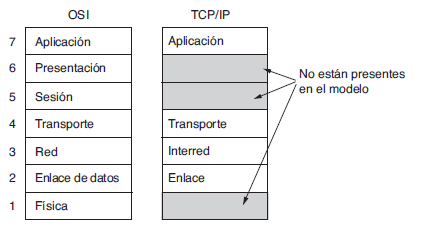
\includegraphics{comptcposi}
	\caption{Comparativa entre modelo OSI y TCP/IP}
	\label{fig:comp_tcposi}
\end{figure}

El modelo OSI, define tres partes básicas: 
\begin{enumerate}
	\item Servicios 
	\item Interfaces 
	\item Protocolos
\end{enumerate}

El modelo OSI, define bien estas tres partes, y las distingue de una manera clara, cosa que no realiza el modelo TCP/IP. Sin embargo, los protocolos del modelo OSI, son difíciles de implementar, por esto se opta por los protocolos que se definen en el modelo TCP/IP. 

Una diferencia importante, se observan en la figura \ref{fig:comp_tcposi}, en el que se observa que el modelo TCP/IP tiene cuatro capas, mientas el otro tiene siete. Una ventaja, en el modelo OSI, es que el protocolo de una capa, puede cambiarse con facilidad, sin afectar las demas capas, esto no es así en el modelo TCP/IP. 

Otra diferencia está en área de comunicación orientada a la conexión y no orientada a la conexión. El modelo OSI soporta ambas comunicaciones en la capa de transporte. Em modelo TCP/IP solo tiene un modo en la capa de red(no orientado a la conexión),pero soporta ambos modos en la capa de transporte, lo que da a los usuarios la oportunidad de elegir, en casos de protocolos sencillos de solicitud-respuesta.  




\section{Protocolo IP} 
%protocolo IP RFC 1958
La capa de red, se encarga de llevar todos los paquetes a destino. Podría ocurrir, que existan varios enrutadores en el medio. Esto contrasta con la capa de enlace de datos, que asegura la fiabilidad de un extremo a otro de un cable. El protocolo IP, se encuentra en el estandar RFC 1958, y es de acceso público. Este protocolo se denomina IP por las siglas ''Internet Protocol''. 

La comunicación en internet funciona de la siguiente manera: la capa de transporte, fragmenta los datos de la capa superior, y se los transmite a la capa de red. Los enrutadores, reenvian cada paquete, a través de mas de un enrutador, hasta llegar a destino. En el destino, la capa de red entrega los datos a la capa de transporte y se los envía a la capa de aplicación. Cuando todas las piezas llegan finalmente a la máquina de destino, la capa de red las vuelve a ensamblar para formar el datagrama original. Un datagrama es la información que viaja en una red, y esta compuesta por números binarios. Si bien, esta definición es bastante burda, es suficiente para el presente trabajo. El datagrama IP, se muestra en la figura siguiente 
% datagrama Ip 

\begin{figure}[ht]
	\centering
	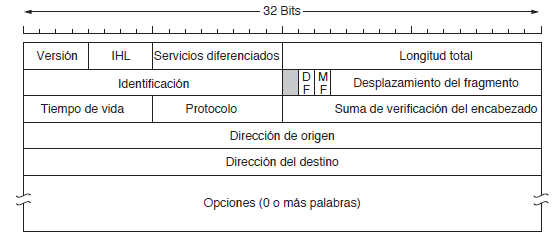
\includegraphics{parte_2/redes/datagip}
	\caption{Datagrama IP}
	\label{fig:datIP}
\end{figure} 
Este datagrama, se compone de dos partes: encabezado y carga útil. El encabezado, se compone de 20 bytes fija y una parte opcional de longitud variable. Los bits se transmiten de izquierda a derecha, y de arriba hacia abajo en la figura \ref{fig:datIP}. Todos los parámetros, están definidos en el estándar mencionado al principio de esta sección, en este trabajo, solo nos concentramos en dos parámetros: Dirección origen y Dirección destino. Estas son las que debemos utilizar para configurar el software, y que las estaciones de trabajo puedan conectarse a nuestro dispositivo. Estas direcciones, se conocen como direcciones IP. 
\subsection{Direcciones IP} 
Si se observa, la figura \ref{fig:datIP}, se observa que hay 32 bits(o 4 bytes) para indicar esta direcciones. Estas direcciones están compuestas de una porcion de longitud variable para indicar la red en los bits superiores, y de una porcion de host en los bits.La porción de red tiene el mismo valor para todos los hosts en una sola red, como una LAN Ethernet. Esto significa que una red corresponde a un bloque contiguo de espacio de direcciones IP.A este bloque se le llama prefijo. 

Las direcciones IP se escriben en notación decimal con puntos. En este formato, cada uno de los 4 bytes se escribe en decimal, de 0 a 255. Por ejemplo, la dirección hexadecimal 80D00297 de 32 bits se escribe como 128.208.2.151.  
inferiores. para escribir los prefijos, se proporciona la ip menor en el bloque y tamaño del mismo. El tamaño se determina mediante el número de bits en la porción de red, los restantes bits(bits de host) pueden variar. Esto significa, que el prefijo debe ser potencia de dos. Por convención, el préfijo se escribe despues de la ip, con los bits dedicados a los host. Por ejemplo, la siguiente notación 128.208.0.0/24, significa que hay 24 bits para la red, y 8 bits para el host. 

Como el prefijo que indica la red, puede ser de longitud variable, entonces se debe realizar una operación and binario con un numero de unos en la parte de red, y ceros restantes.Este número con el que se realiza esta operación, se denomina \textbf{mascara de subred}. En el ejemplo anterior: 128.208.0.0/24, la mascara de subred es en decimal: 255.255.255.0. Si realizamos la operación and bit a bit entre 255.255.255.0 y 128.208.0.0, obtenemos 128.208.0.0, lo cual indica que pertenece a la red 128.208.0.0. En este trabajo, solo requerimos de estos conceptos, para configurar el software de cada estación de trabajo, y realizar la conexión con el dispositivo desarrollado en el presente trabajo.     
 
\section{Protocolo DHCP} 

De la sección anterior, se obtiene que cada computadora, estación de trabajo, o dispositivo que se conecte a la red, debe al menos configurarse la dirección IP, y la mascara de subred, para que puedan intercambiar mensajes entre ellos, o utilizar cualquier servicio disponible en la red. Esto, puede resultar un proceso tedioso, por esto, se define en el estándar RFC 2131 un protocolo de asignación dinámicas de ips, conocido como DHCP(Protocolo de Configuración Dinámica de Host,
del inglés Dynamic Host Configuration Protocol). En el estandar, están definidas la forma de comunicación para obtener estos datos, que es básicamente la dirección IP asignada de manera automática.  
Dentro de cada red, debe existir un servidor DHCP. para iniciar la solicitud, la máquina, envía a través de la red, una solicitud, denominada DHCPDISCOVER.Si el servidor esta disponible, envía la dirección en un paquete denominado DHCPOFFER. 
Un paquete DHCP esta conformado por los bits que se muestran en la figura \ref{fig:pqdhcp}: 
\begin{figure}[ht]
	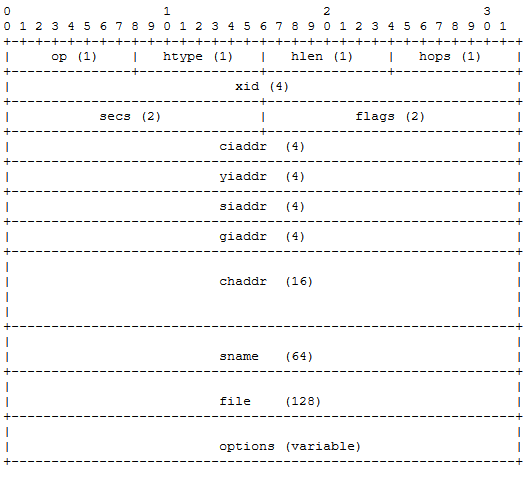
\includegraphics[width=\textwidth,height=10cm]{paqdhcp}
	\caption{Datagrama para intercambio de mensajes del protocolo DHCP}
	\label{fig:pqdhcp}
\end{figure} 

Estos parámetros, son bits, los cuales deben enviarse a través de la red. Estos campos de bits, no serán explicados, ya que están implementados dentro de la libreria W5100 que maneja el entorno de arduino UNO. Estos bits están descritos en el estándar indicado en el primer párrafo de la esta sección, y son de acceso público. 


\section{Protocolo TCP } 
Este protocolo, pertenece a la capa de transporte. Se diseño especificamente para proporcionar un flujo de bytes confiable de extremo a extremo a través de una interred no confiable. Una interred difiere de una sola red debido a que sus diversas partes podrían tener diferentes topologías, anchos de banda, retardos, tamaños de paquete y otros parámetros. TCP se diseñó para adaptarse de manera dinámica a las propiedades de la interred y sobreponerse a muchos tipos de fallas.

%para conocer la importancia de este protocolo dentro de las redes, se ha definido el primer estandar RFC 793, en el año 1981. Luego de este documento, se han definido varias mejoras: 
%\begin{enumerate}
%	\item RFC 1122: aclaraciones, y correcciones de errores  
%	\item RFC 1323: extensiones para alto desempeño 
%	\item RFC 2018: confirmaciones de recepción selectivas 
%	\item RFC 2581:control de congestión 
%	\item RFC 2873 readaptacion de los campos del encabezado para la calidad del servicio 
%	\item RFC 2988: temporizadores de transmisión mejorados 
%	\item RFC 3168: notificación explícita de congestión 
%\end{enumerate} 

%Las normas RFC, son solo algunas de las relacionadas al protocolo TCP.Debido a la gran cantidad de normas generadas para este protocolo, se ha definido un nuevo documento que los ordena a todos estos:el RFC 4614.  

La capa IP no ofrece ninguna garantía de que los datagrama se entregarán de manera apropiada, ni tampoco una indicación sobre qué tan rápido se pueden enviar los datagrama. Corresponde a TCP enviar los datagramas con la suficiente rapidez como para hacer uso de la capacidad sin provocar una congestión; también le corresponde terminar los temporizadores y retransmitir los datagramas que no se entreguen. 

\subsection{Servicio TCP}
	El servicio TCP se obtiene al hacer que tanto el servidor como el receptor creen puntos terminales, llamados sockets. Cada socket tiene un número (dirección) que consiste en la dirección IP del host y un número de 16 bits que es local para ese host, llamado puerto. Un puerto, es definido por la capa de aplicación, que es el punto de acceso a la capa de aplicación. para obtener el servicio TCP, hay que establecer de manera explícita una conexión entre un socket en una máquina y un socket en otra máquina. 
	Existen puertos que se denominan ''conocidos'', y son casi un estándar, por ejemplo el puerto 80 para el protocolo HTTP. Los puertos definidos van de 0 a 1024. Los puertos de 1024.Los puertos desde el 1024 hasta el 49151 son puertos que se pueden registrar en IANA, pero las aplicaciones son las que seleccionan sus propios puertos.  
	Todas las conexiones TCP son full dúplex y de punto a punto. Full dúplex significa que el tráfico puede 	ir en ambas direcciones al mismo tiempo. Punto a punto significa que cada conexión tiene exactamente dos puntos terminales. TCP no soporta la multidifusión ni la difusión. 
	La entidad TCP emisora y receptora intercambian datos en forma de segmentos. Un segmento TCP consiste en un encabezado fijo de 20 bytes (mas una parte opcional), seguido de cero o mas bytes de datos. El software de TCP decide qué tan grandes deben ser los segmentos. Puede acumular datos de varias escrituras para formar un segmento, o dividir los datos de una escritura en varios segmentos. Una cabecera esta formada de la siguiente manera: 
	\begin{figure}[ht]
		\centering 
		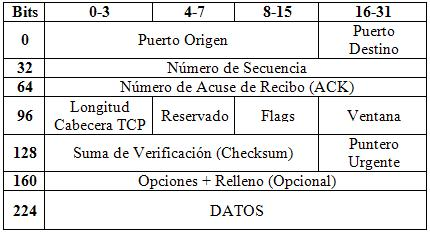
\includegraphics[height=4cm,width=0.6\textwidth]{parte_2/redes/cabecera-tcp} 
		\caption{Cabecera del protocolo TCP}
	\end{figure}

	En el encabezado TCP, se tiene puerto origen, puerto destino. Observando, el datagrama de la figura \ref{fig:datIP}, tenemos dos IPs: IP origen, e IP destino, y el protocolo TCP, tiene dos puertos(origen y destino), y el mismo protocolo. Este identificador de conexión se denomina 5-tupla,ya que cinco elementos son los que participan. 
	Por último, cabe destacar, que los puertos y los datos, los define el programador o software, en la capa de aplicación. El programador al usar el protocolo TCP, no debe realizar una verificación de los datos, ya que el protocolo mismo, se encarga de esto. 
	
	Estos elementos, se definen, ya que son necesarios para poder avanzar en los conceptos en el presente trabajo, ya que en un futuro, se deben configurar los software de los usuarios, y la programación del microcontrolador seleccionado en el capítulo anterior, basados en estos conceptos para poder realizar una integración exitosa, entre el microcontrolador y las computadoras del lugar. 
	
\section{Sniffer de red -WireShark} 

Un programa que pueda revisar los paquetes de una red que llegan a una computadora, y los pueda visualizar, se denomina sniffer. Un sniffer de red, no es mas que un software, en el cual se pueden visualizar los paquetes recibidos, en la computadora que esta instalado. El software elegido para realizar esta visualización de los paquetes se llama WireShark. Se ha elegido este software, dado que es software libre, y pueden filtrarse los paquetes por puertos, y por IP. Ademas tiene muchas otras opciones que no serán contadas, ya que no se utilizan en el desarrollo del dispositivo. En la primera pantalla, se debe seleccionar la placa de red de la PC (podría tener para de una), en la que se encuentra instalado, y luego puede realizar un análisis. A continuación se muestra una imagen de un análisis hecho sobre una PC.
%\setlength{\textheight}{290mm}
\begin{figure}[H]
	\centering 
	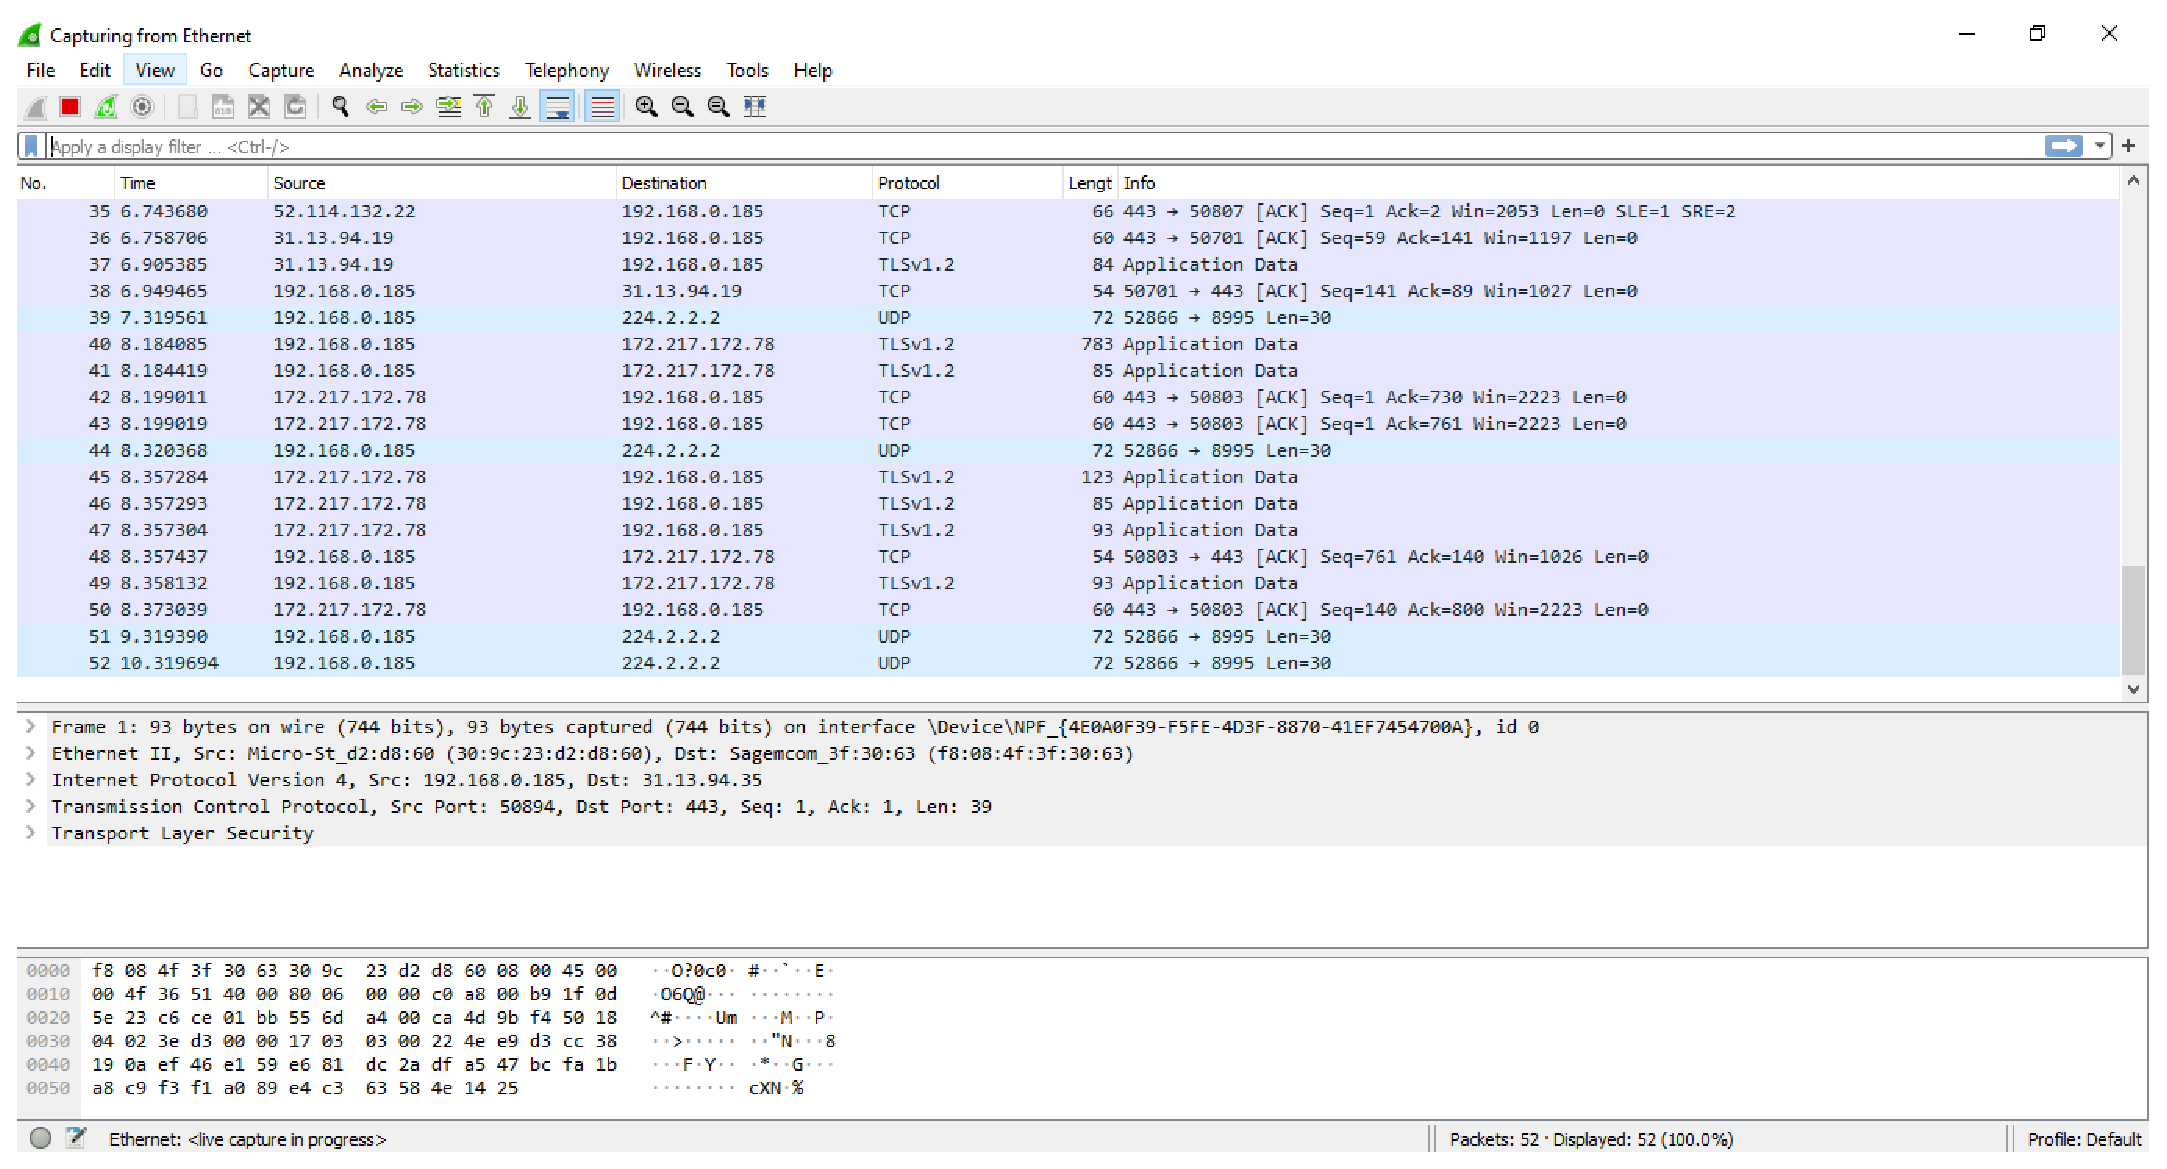
\includegraphics[height=7cm]{wireshark}
	\caption{análisis de los datos dentro de una red utilizando WireShark}
\end{figure}


Como se ve en la figura, se observa IP de origen, Ip de destino, y ambos puertos, y ademas el paquete TCP reensamblado, y el tipo de protocolo utilizado para la comunicación.  

Este software, se va a utilizar, para comprobar la conexión de los programas para que realicen seguimiento de satélites. Ademas, se puede comprobar los protocolos implementados por los programas. 


\graphicspath{{parte_2/Interfaz de usuario}}

\renewcommand{\chaptername}{interfaz de usuario}

\chapter{Interfaz De usuario} % \label{cap:int_user}
\markright {Interfaz de usuario	}
\begin{center}
	\begin{tcolorbox}[colback=gray!5!white, %Color del fondo
		colframe=blue!75!black,
		title= \center{\Large{resumen}} ]
		Se van a definir las interfaces sobre las computadoras de la institución. Estas interfaces, se basan en software existente. Para seleccionar las interfaces, se realiza una comparación de todos estos. Luego de esto, se va a mostrar cómo realizar la configuración de los dos software seleccionados.   
	\end{tcolorbox}
\end{center}    



\section{introducción}
En esta sección, analizamos los programas que son capaces de mostrar las posiciones de los satélites en tiempos real. Luego de un análisis, se seleccionan dos de estos mismos. Los programas existentes deben tener capacidad de enviar las posiciones de los satélites usando la red local de la institución. Luego del análisis de los programas, se muestran cuáles deben ser los pasos a seguir para poder configurar dichos programas.  

\section{Interfaz de Usuario}

La figura \ref{fig:fig_ssgen}, se observa que hay estaciones de trabajo. En esta sección, definimos el software de seguimiento de satélites, para las estaciones de trabajo del lugar. Algunos de los software que se analizan fueron obtenidos desde la página web de la AMSAT (asociación mundial de satélites de radioaficionados),y otros desde la investigación a través de Internet. 
Los distintos programas que se analizan son: 
\begin{itemize}
	\item Gpredict 
	\item Stelarium 
	\item Orbitron 
	\item Celestia 
	\item Pass 
\end{itemize}
Hay que destacar, que todos estas aplicaciones, requieren la ubicación del usuario(en este caso, de la antena), en sistemas de coordenadas terrestres(latitud y longitud del lugar, con su respectivo signo). 


\subsection{Orbitron}
Este software permite la ubicación de satélites en tiempo real, permite simulaciones donde se pueden observar el día y la hora aproximada de llegada del satélite al plano del horizonte(ver capítulo \ref{cap:sist_cord}) donde se encuentre la antena. 
Además, permite que observar la posición del sol y la luna en tiempo real. 

\begin{figure}[ht]
	\centering
	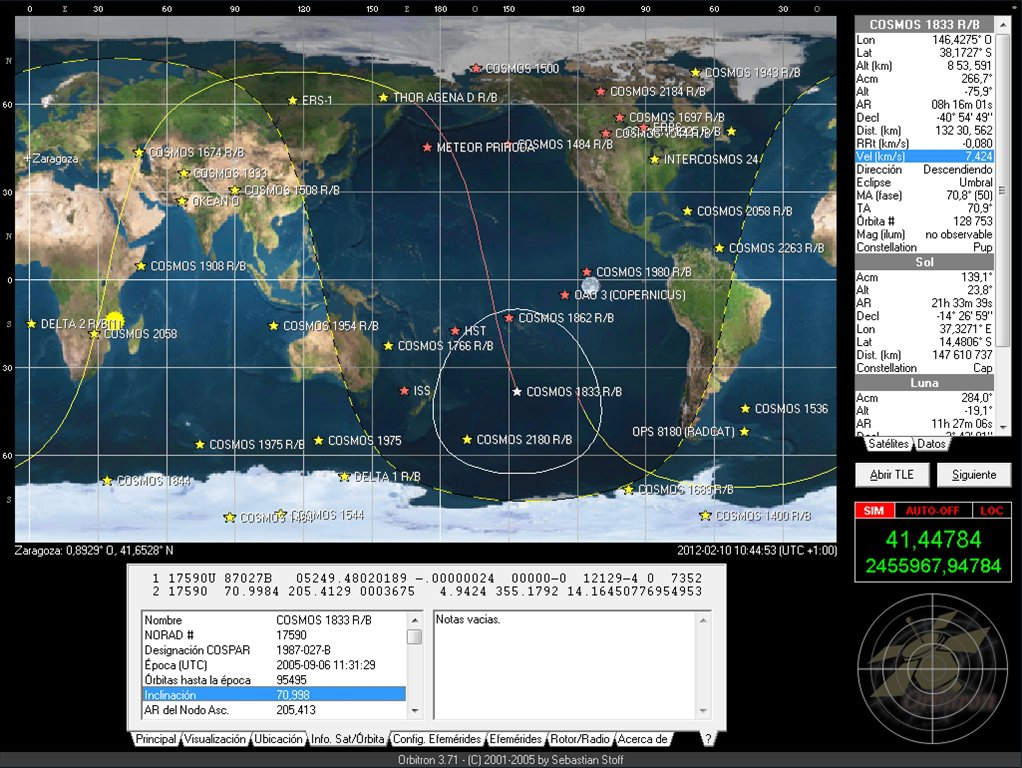
\includegraphics[scale=0.4]{orbitron}
	\caption{Captura de pantalla del software Orbitron }
\end{figure}

Como contra de este software, es que no permite realizar el seguimiento de estrellas, y no puede conectarse a la red, para enviar estos datos a través de la red local. Solo tiene conexión con los puertos(puertos USB) de la PC para obtener los datos. Para poder enviar estos datos, a través de la red, se debe simular un puerto virtual, obtener esos datos, y enviarlos a través de la red local. Es decir, requiere un programa que haga de intermediario. 

\subsection{Stellarium} 
El software stellarium, posee un seguimiento en tiempo real de estrellas, y está pensado para realizar el seguimiento usando telescopios. Tiene distintos módulos, lo que lo hacen personalizable. Tiene soporte para estrellas, y satélites. Estos datos, pueden enviarse a través de la red, para que los reciba un telescopio, y realice el apuntado del telescopio. Existen pluggins, de este software, que permiten enviar las coordenadas a dispositivos mediante la red. Una imagen del software puede visualizarse en la siguiente figura:% \ref{fig:stelarium_init}  

\begin{figure}[ht]
	\centering
	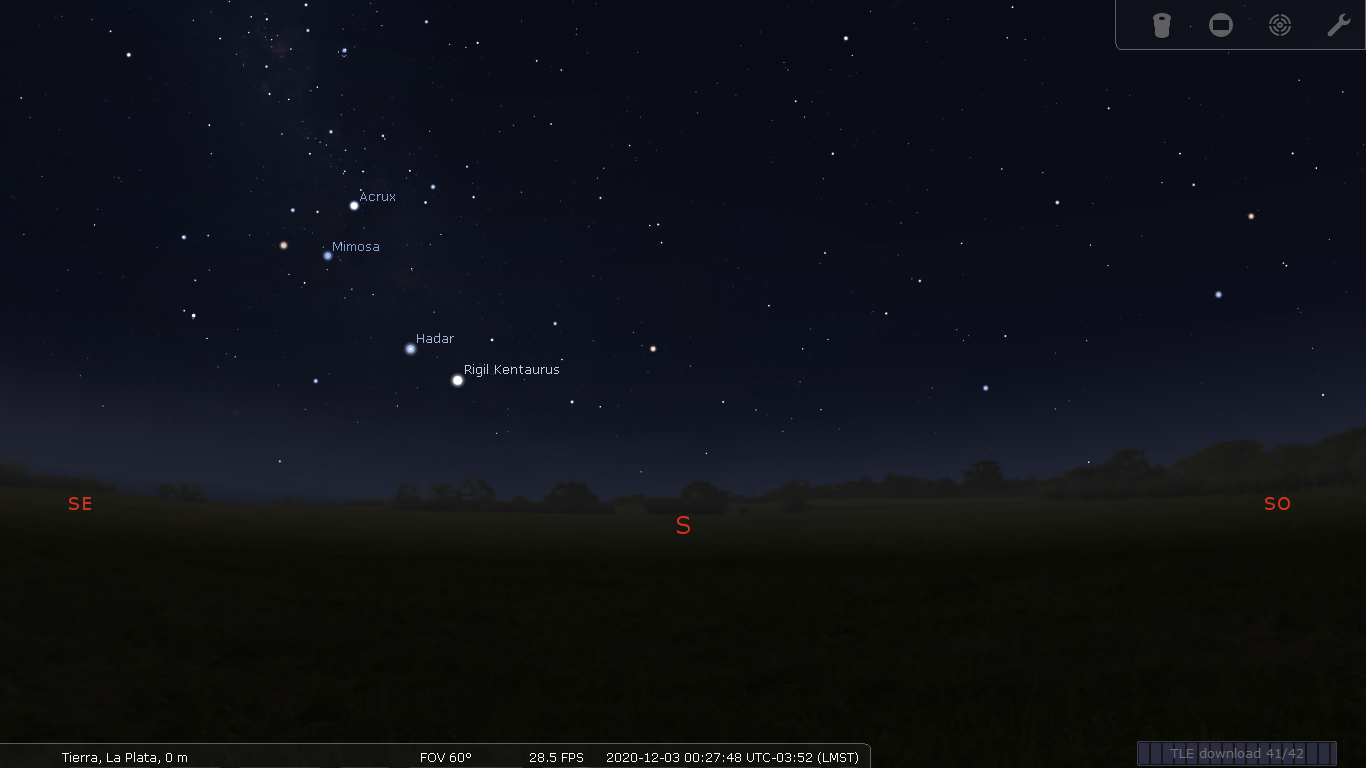
\includegraphics[width=\linewidth,height= 5.6cm]{stellarium}
	\caption{Imagen al abrir el software Stellarium }
	\label{fig:stelarium_init}
\end{figure}




\subsection{Celestia} 
Celestia es un software, que permite realizar ``viajes'' a las estrellas. Este software tiene un fin educativo, puede realizar algunas simulaciones, y se puede viajar al ``espacio a donde uno desee''. Este software no posee ningún tipo de comunicación con el exterior. 
\begin{figure}[ht]
	\centering
	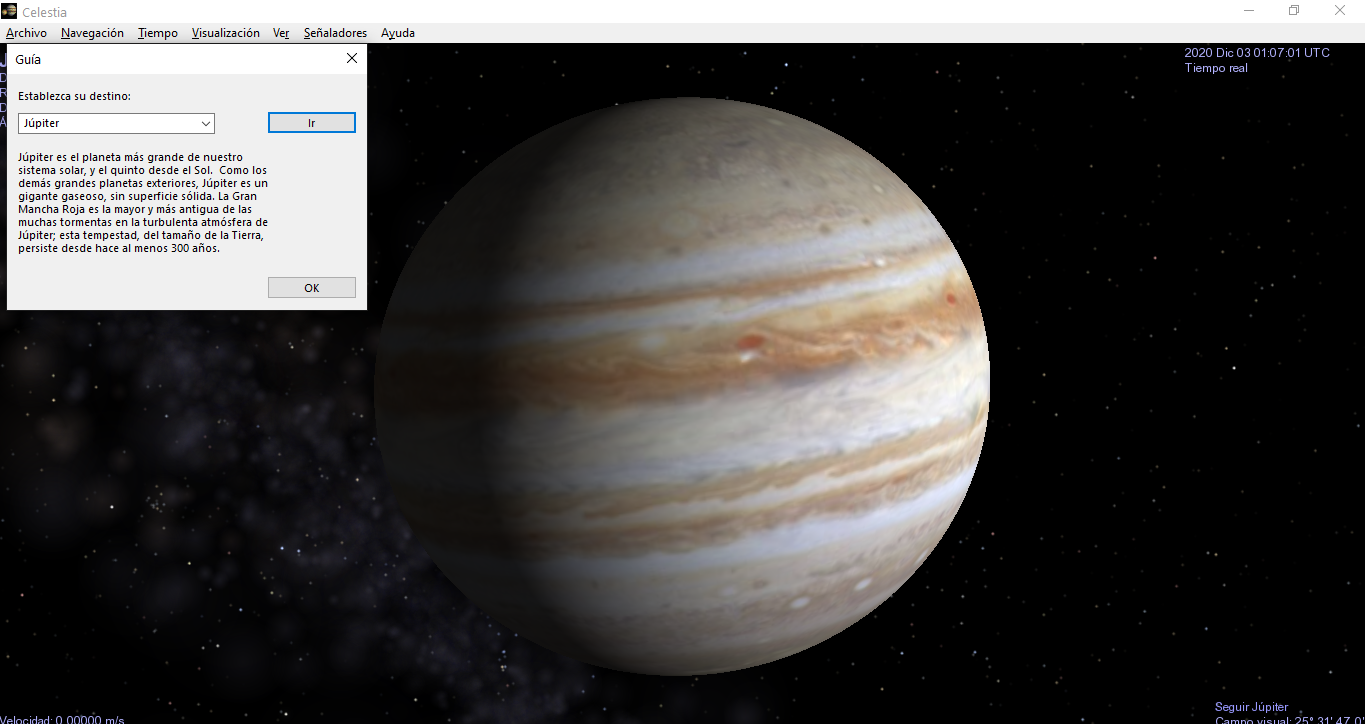
\includegraphics[scale=0.3]{celestia}
	\caption{Viaje a júpiter a través de celestia}
\end{figure}



\subsection{Pass}
Pass no es una aplicación para PC en sí. Es una página web con todos los satélites encima de un mapa. La página es http://amsat.org.ar/pass. La captura de pantalla se muestra en la siguiente figura:% \ref{fig:iu_pass}.
\begin{figure}[ht]
	\centering
	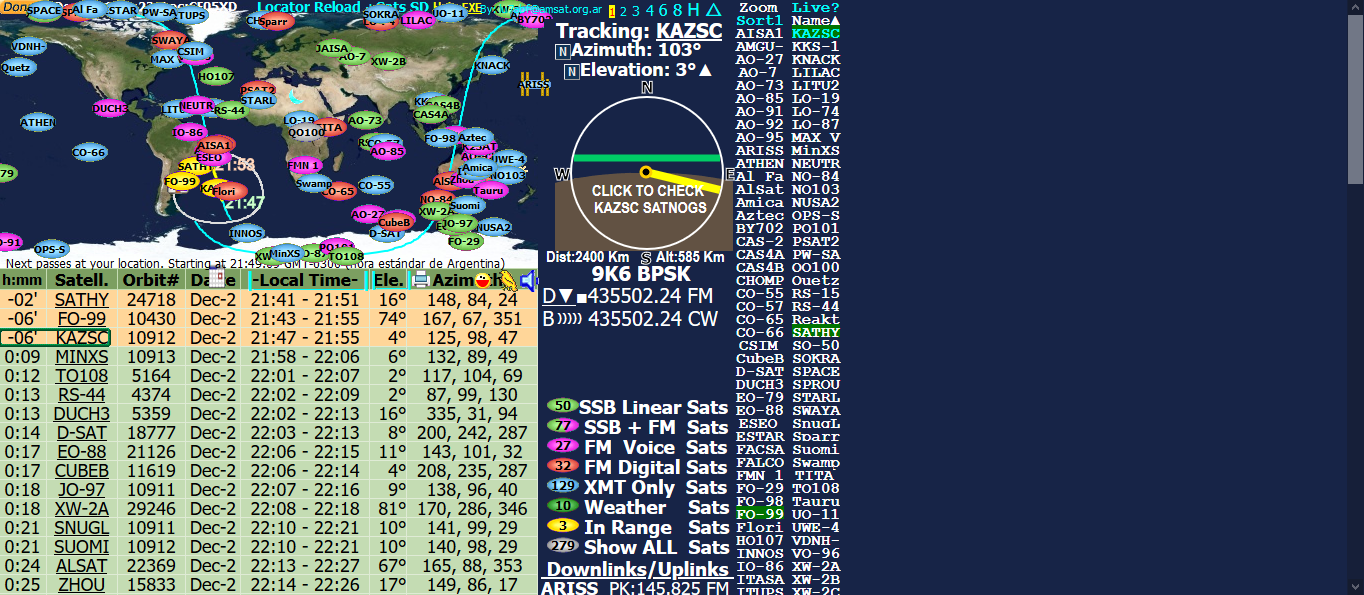
\includegraphics[width=\linewidth, height= 6cm]{pass}
	\caption{Captura de pantalla de la página http://amsat.org.ar/pass }
	\label{fig:iu_pass}
\end{figure}

Éste software, obtiene la geolocalización a partir de la conexión a Internet. A partir, de ellas, obtiene la orientación de la antena. Debido a que obtiene las coordenadas a partir de la conexión a Internet, se tiene un error en el apuntamiento de la antena, ya que estas coordenadas están desfasadas respecto a las reales.    

\subsection{Gpredict}

El software Gpredict es un software que muestra en tiempo real las ubicaciones de los satélites dentro de un mapa, que permite, la configuración de sistemas receptores y sistemas de rotación para antenas. El mismo es libre, su código fuente está disponible en Internet, como así su programa compilado, el mismo puede usarse en Windows y Linux. Este, provee una base de datos de satélites, y se actualiza con la frecuencia que se configure. Además, soporta envió de datos mediante el uso de una red local, configurando sus parámetros. Una captura de pantalla puede verse en la siguiente figura:  %\ref{fig:iu_gpredict}.

\begin{figure}[h]
	\centering
	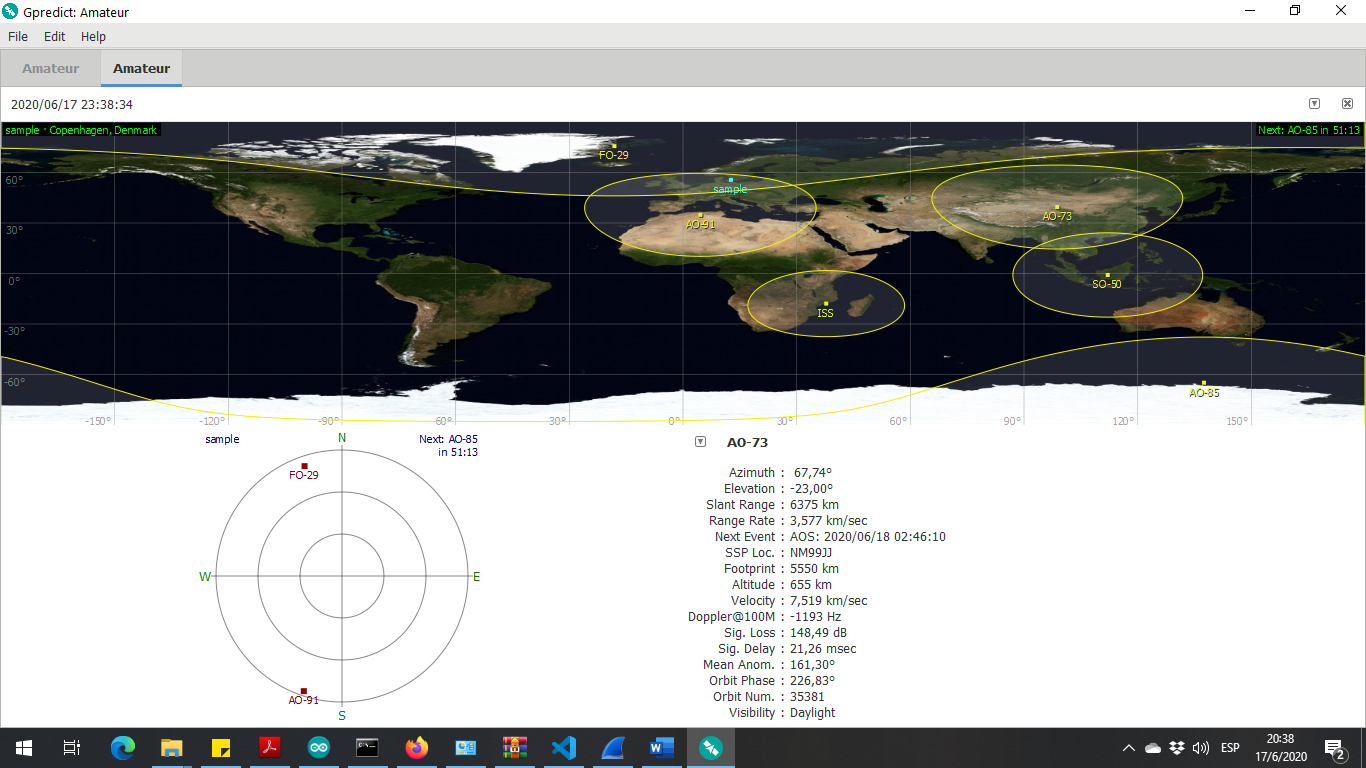
\includegraphics[width=\linewidth,height=7cm]{gpredict}
	\caption{Captura de pantalla del software Gpredict}
	\label{fig:iu_gpredict}
\end{figure}


\section{Comparativa de interfaces y selección del software}
Una vez, realizado el análisis sobre cada aplicación, se realiza una tabla comparando sus características(ver tabla \ref{tab:comp_soft})
\begin{table}[htb]
	\centering
	\begin{tabular}{|c|c|c|c|c|c|}
		\hline
		Software 			& Orbitron & Gpredict & Celestia & Stelarium & pass\\ 
		\hline
		Posición Geográfica & Sí 	   & Sí 	  & No 		 & Sí        & Sí  \\
		\hline
		Soporte para redes  & No 	   & Sí       & No       & Sí        & No  \\
		\hline
		Satélites 			& Si 	   & Sí		  & No		 & Sí	 & Si  \\
		\hline
		Estrellas 			& No	   & No		  &Sí		 & Sí		 & No  \\
		\hline	
\end{tabular}
\caption{Comparativa entre los distintos software} 
\label{tab:comp_soft}
\end{table}

De la tabla, se observa que hay dos programas que pueden usarse sin ningún complemento adicional: Gpredict y Stellarium. El stellarium es un software pensado para telescopios, pero conociendo su protocolo, puede obtenerse las coordenadas para apuntar una antena, pues el software no es capaz de reconocer el tipo de dispositivo que debe apuntar. El Gpredict, es un software especializado en seguimiento de satélites en tiempo real. En lo que resta del presente texto, se utilizará el software Gpredict y el Stellarium para realizar el apuntamiento de la antena. 
 


\section{Software Gpredict} 
El software Gpredict, se basa en el software libre. Su código fuente está disponible para descargarse y compilarse, o puede descargarse directamente el archivo binario compilado. Tiene soporte para entornos Windows y Linux. Su lenguaje es C, y se basa en la librería GTK para el entorno gráfico. El software, posee un código que calcula las futuras posiciones de los satélites, en base a modelos matemáticos dentro de su código, estas se actualizan según se actualice su base de datos de satélites. Estas bases de datos se actualizan con frecuencia predeterminada por el usuario.  
Para el soporte de red, su software basa su comunicación en la librería llamada HAMLIB, disponible en varios lenguajes de programación para usarse. Esta librería, propone su propio protocolo de comunicación a través de la red, además tiene funciones relacionadas al ajuste de los receptores de comunicaciones mediante la conexión a la red local.   

\subsection{Libreria Hamlib}
Hamlib es una capa de software dedicada al manejo de radios y rotadores \footnote{Un rotador es un dispositivo que es capaz de mover la antena en la dirección que se le ordene.}de tipo comercial, y no comercial. Esta capa de software actúa por debajo de las interfaces gráficas, y aplicaciones de usuario. El software principal(en este caso Gpredict), llama a esta librería para comunicarse con los dispositivos de radio o rotadores. 

Esta capa de software se relaciona con distintos tipos de radios, y tiene protocolos comerciales(algunos, se debe ver la lista de dispositivos soportados) ya implementados. Además, permite la incorporación de dispositivos que aún no estén implementados, ya que puede descargarse su código fuente desde Internet. 

Esta librería, define cuatro programas para realizar pruebas, estos programas son: 
\begin{itemize}
	\item rigctl: manejo de radios por puerto serie 
	\item rotctl: manejo de rotadores por puerto serie
	\item rigctld: manejo de radios mediante el protocolo TCP/IP
	\item rotctld: manejo de rotadores mediante el protocolo TCP/IP
\end{itemize}

Los dos últimos de la tabla anterior, son los que tienen interés dentro de este documento. Al realizar la opción de seguimiento de satélites, internamente Gpredict, llama a ``rotctld'', y mediante un protocolo de comunicación documentado dentro de la documentación oficial de Hamlib, se realiza el intercambio de mensajes entre la aplicación y el rotador. 

\subsubsection{Protocolo de comunicación} \label{subsub:protocol_com}
El protocolo de comunicación implementado dentro del programa ``rotctld'' se basa en texto plano, separado por espacios en blanco, y tiene un carácter de fin de mensaje, con el carácter salto de línea, o conocido como ``\textbackslash{}n'' dentro del código ASCII. 

Existen dos tipos de comandos: los denominados métodos Get y Set. Los primeros obtienen información del rotador, mientras los últimos, le envían información al rotador que es lo que debe realizar. Algunos de los comandos utilizados por este programa(Gpredict en conjunto con rotctld) son los siguientes: 

\begin{table}[H]
	\centering
	\begin{tabular}{|c|p{5cm}|c|p{5cm}|}
		\hline
		\multicolumn{2}{|c|}{Metodos Get}  &  \multicolumn{2}{c|}{Metodos Set}  \\ 
		\hline
		Comando & Descripción & Comando & descripción	\\
		\hline
		p & Obtener posición actual del rotador  &P& Enviar posición al rotador \\
		\hline 
		q & Desconectar el rotador 	Cierra la conexión & S & Parar el rotador \\ 
		\hline 	
	\end{tabular}
	\caption{Comandos de rotctld usados por Gpredict} 
	\label{tab:commands_Gpredict}
\end{table}

Además de estos comandos, existen un comando que no encaja en la categoría de Get o Set, es el comando M, que le indica la velocidad de seguimiento de la antena, este no esta disponible en Gpredict. 

Esta librería, además, posee un formato de respuesta, el cual se establece con separadores de espacio en blanco, y terminados en un salto de línea, para el caso de métodos GET. Estos métodos, piden información al rotador, y está definida cada respuesta dentro del manual de HAMLIB. Estas, pueden verse en su manual(vea referencia \cite{HAMLIBDOC}). 

\subsection{Selección de satelites y creación del perfil} 

El software Gpredict, permite seleccionar los satélites a realizar seguimiento mediante la elección de los mismos, y creando lo que se denominan ``módulos''. Cada módulo puede seleccionar los satélites a seguir, además, pueden agregarse satélites a seguir, añadiendo la base de datos manualmente.

Al iniciar el software(ver figura \ref{fig:iu_gpredict}) este viene con un módulo predeterminado, que se denomina ``Amateur''. Este viene con algunos satélites precargados. 

Para crear un perfil, debe dirigirse a file $\rightarrow$ new module, como se muestra en la siguiente imagen:% \ref{fig:create_modul_gpred}  
\begin{figure}[ht]
	\centering
	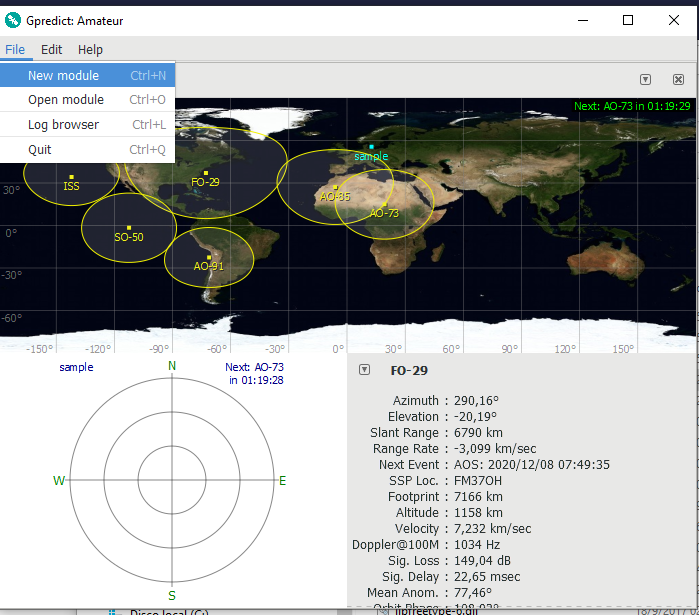
\includegraphics[width=\textwidth,height=8cm]{create_module}
	\caption{Creación de un módulo dentro de Gpredict} 
	\label{fig:create_modul_gpred}	
\end{figure}

Al realizar esto, se abre la ventana, dónde selecciona los satélites a seguir. Esta ventana se muestra en la figura \ref{fig:sel_sat}. En esta ventana, seleccionamos los satélites, y lo nombramos al módulo. En este caso, se lo denominamos arduino. 

\begin{figure}[ht]
	\centering
	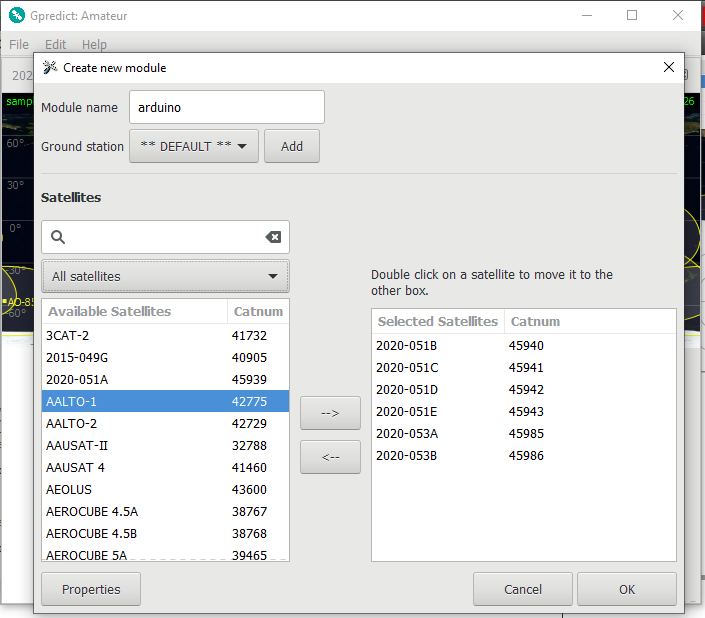
\includegraphics[height=10cm,width=\textwidth]{select_sat}
	\caption{Selección de satélites para el nuevo módulo creado} 
	\label{fig:sel_sat}	
\end{figure}
%\vspace{}
Donde dice ``Ground station'',se debe configurar latitud y longitud de la antena. Luego se presiona OK. Después de esto, ya se creó el módulo. Para abrirlo cuando desee, debe dirigirse a file $\rightarrow$ open module, y elegir ``arduino'' como módulo.
\subsection{Configuración del rotador en Gpredict} \label{subs:conf_Gpredict}
Para configurar el rotador, en la página que se abre al iniciar el programa(ver figura	\ref{fig:iu_gpredict}), debe dirigirse a edit $\rightarrow$ prefences. Al realizar esto, se abre la siguiente ventana: 
\begin{figure}[H]
	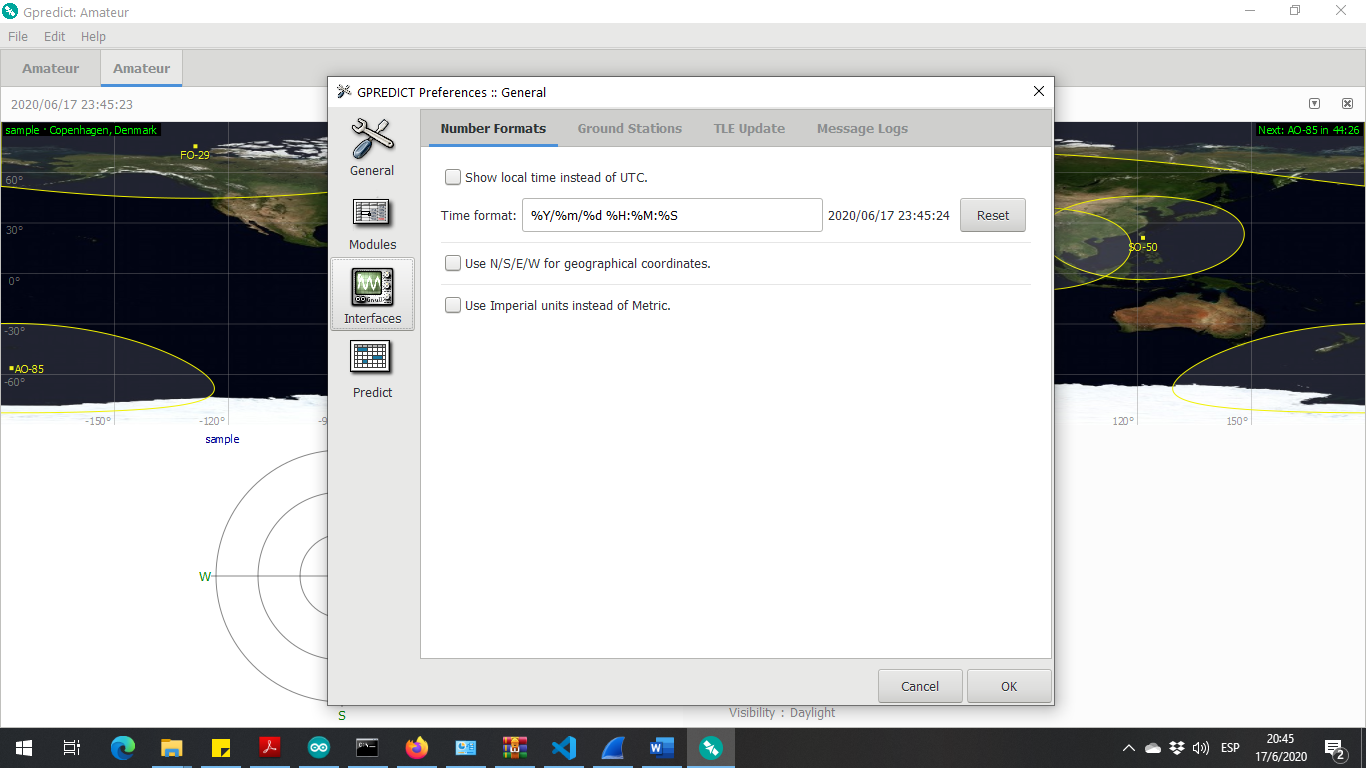
\includegraphics[height=5cm,width=\textwidth]{select_rot}
	\caption{Configuración de rotador}
%	\label{key}
\end{figure} 

Luego de esto, debe presionar en la parte izquierda de la figura anterior, donde dice ``interfaces''. Al realizar esto, debe presionar, en la pestaña ``rotators''. A continuación se la ventana que se abre al presionar sobre interfaces
\begin{figure}[H]
	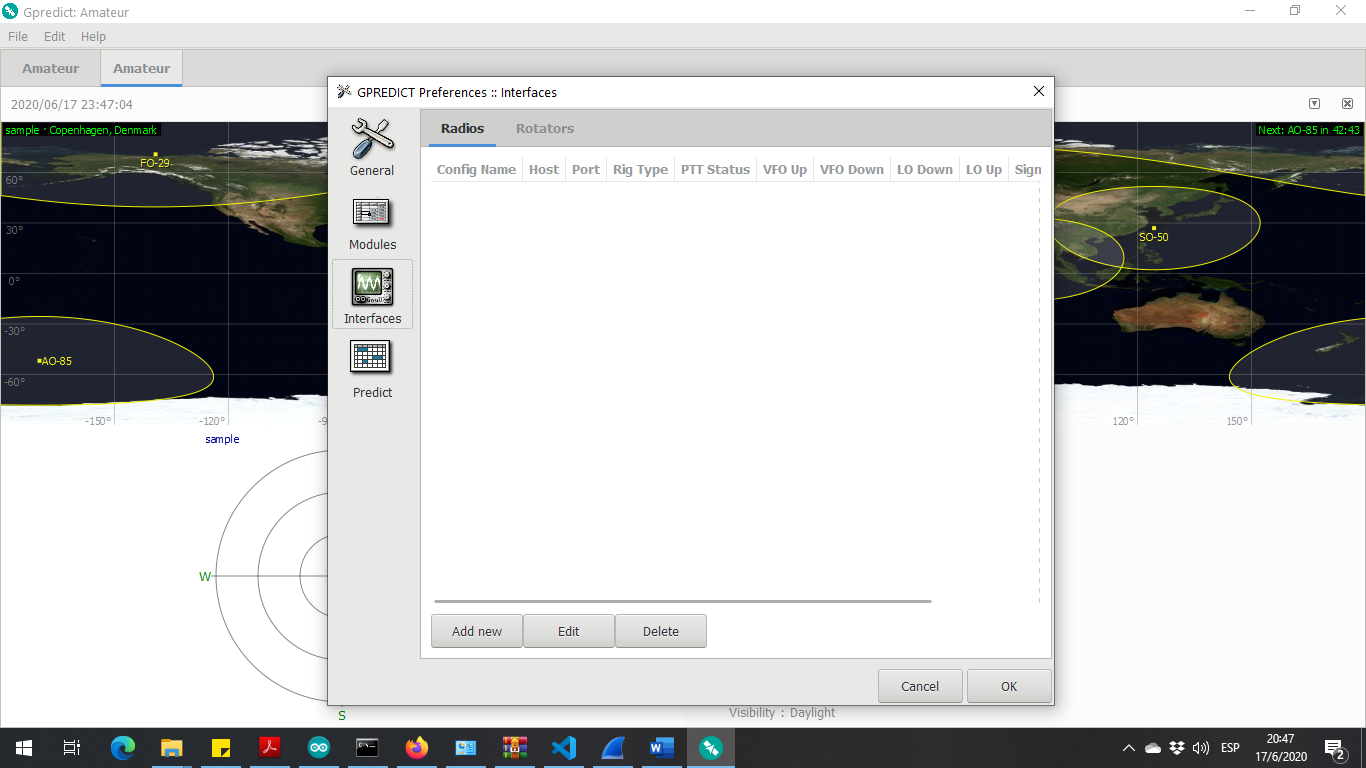
\includegraphics[height=10cm,width=\textwidth]{rotators_int}
	\caption{Configuración de rotador}
\end{figure} 

Luego, debe presionar en la pestaña rotators, y presionar donde dice ``add new'', y se abre una ventana como la que se muestra en la figura \ref{fig:conf_rot_ip}: 

\begin{figure}[h]
	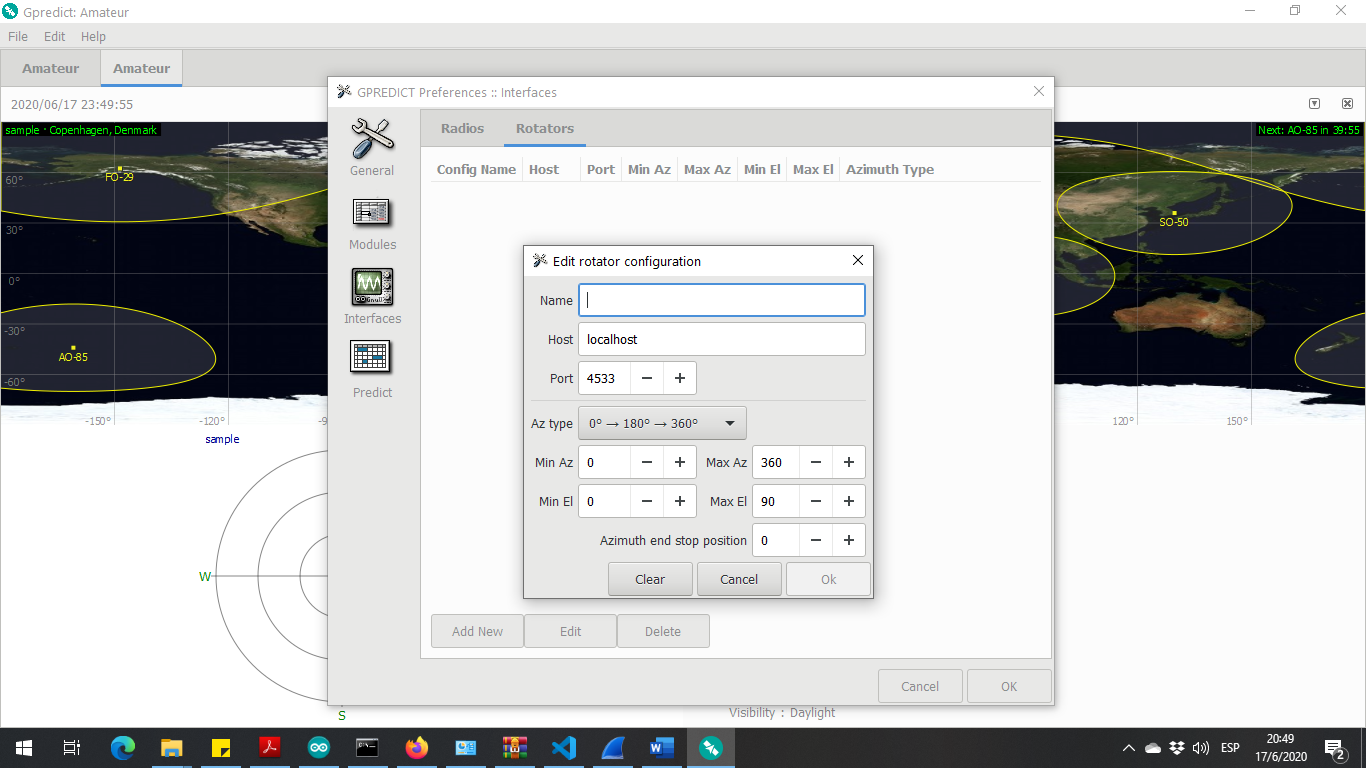
\includegraphics[height=8cm]{conf_rot}
	\caption{Configuración de rotador}
	\label{fig:conf_rot_ip}
\end{figure} 

Los parámetros a configurar son nombre del rotador(el que desee el usuario), ángulos máximos y mínimos de la antena. Estos parámetros se verán en el siguiente capítulo. Además, se observan que se debe definir el host y el puerto. El host, es la IP del dispositivo desarrollado en el presente documento, y el puerto, se define según el gusto del usuario, en nuestro caso, se va a utilizar el puerto por defecto (4533).Luego de rellenar los datos, debe seleccionar OK, y con esto, está configurado el rotador. Se pueden definir tantos rotadores como se deseen, se deben repetir los pasos. 

Una vez creado el rotador,para visualizar el rotador desde la pantalla principal, debe dirigirse a la parte derecha de la pantalla principal, y presionar ahí. En ese lugar, aparece un menú, debe dirigirse a ``antena control'', como se ve en la figura \ref{fig:ant_ctrl} 
\begin{figure}[H]
	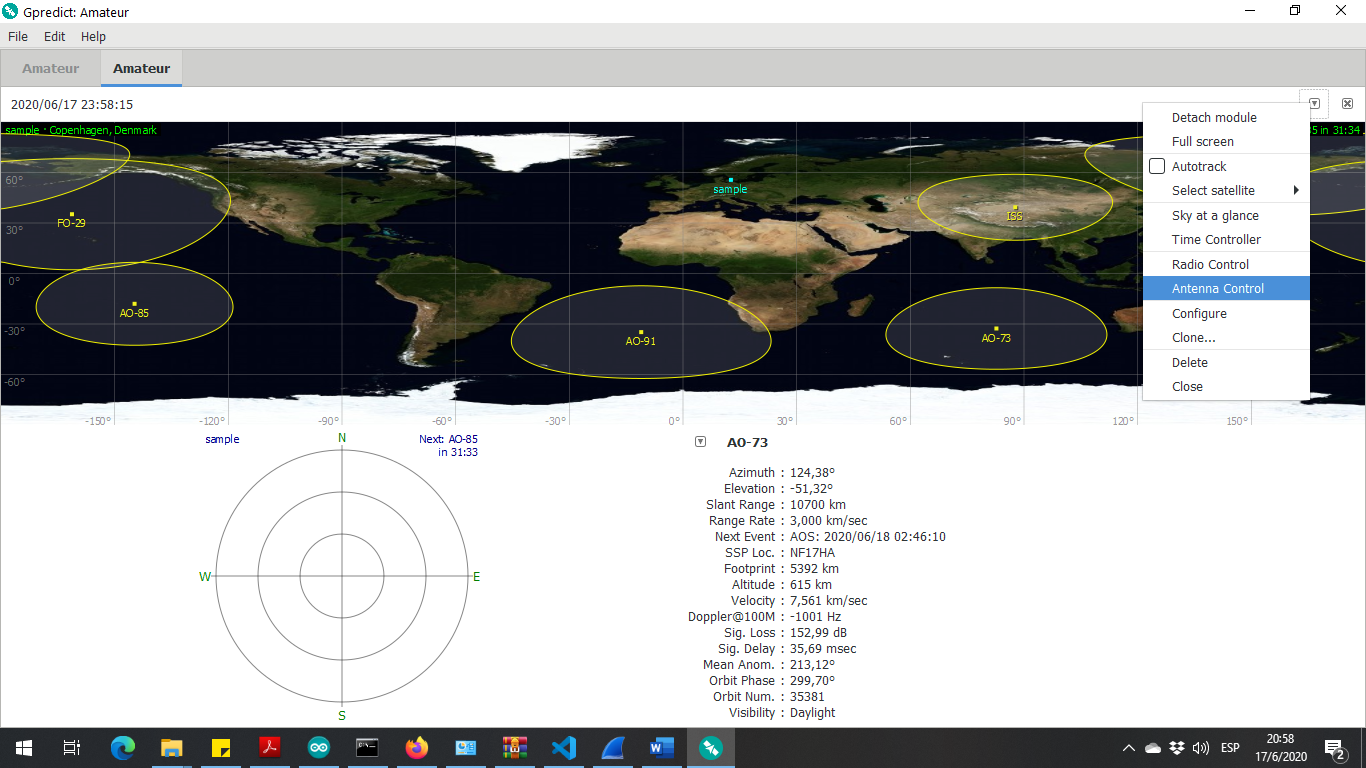
\includegraphics[height=10cm,width=\linewidth]{antena_control}
	\caption{Ver el rotador o rotadores configurados} 
	\label{fig:ant_ctrl}
\end{figure}



Al realizar este paso, aparece el rotador de antena, que se ve en la siguiente figura 

\begin{figure}[H]
	\centering 
	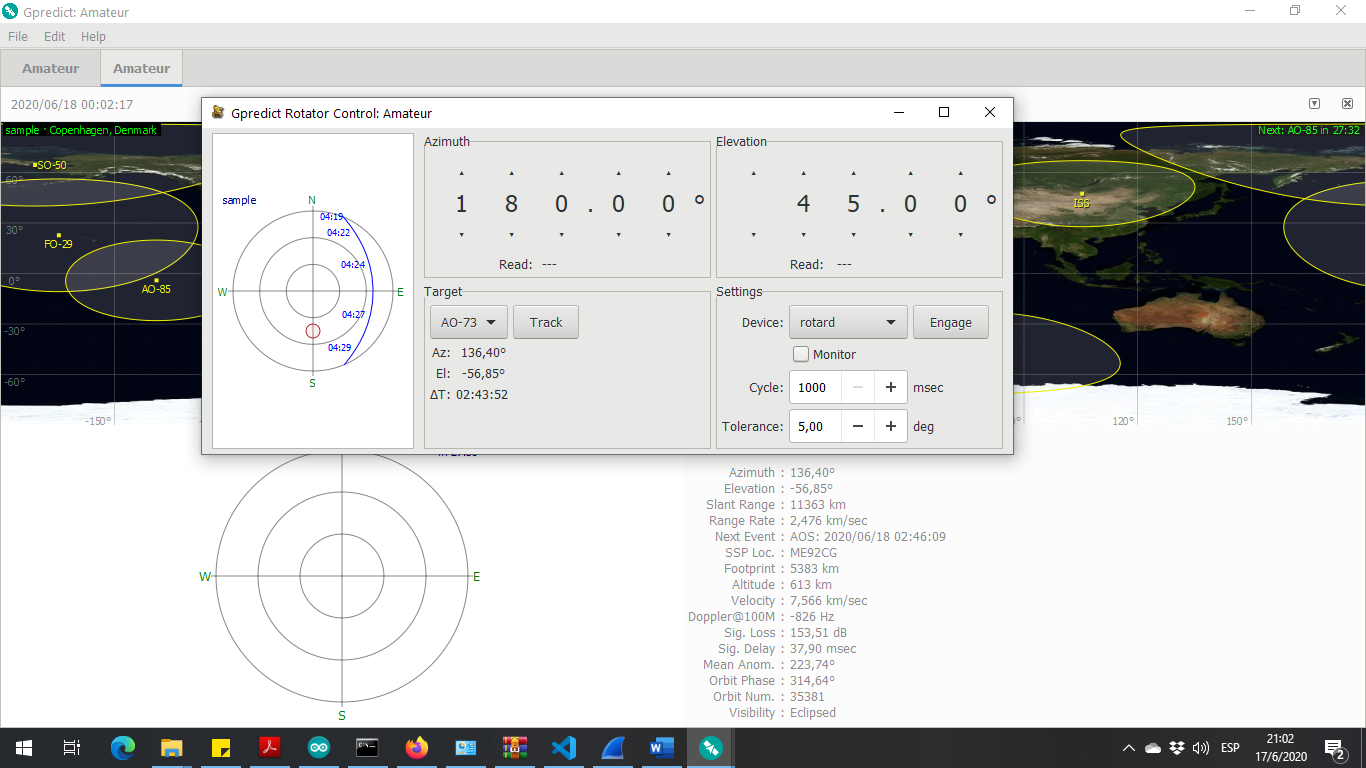
\includegraphics[trim=5.4cm 8cm 9.2cm 2.4cm ,clip,width=\linewidth,height=5cm]{antena_gpr_control}
	\caption{Panel de control del rotador de Gpredict} 
	\label{fig:pan_ctrl_antena}
\end{figure}

En esta figura, se observan dos botones, y dos menús, y un mapa de la antena. Estos dos botones son ``track'' y ``engage''. En el menú de track, realizamos el seguimiento automático. El menú, engage, sirve para realizar la calibración de la antena. El sistema de coordenadas empleado por este software es horizontal-azimutal, con el cero en el polo norte. Estas coordenadas son definidas en la fase 3, donde se muestra el análisis matemático de estas.  

Las medidas angulares, corresponden a los ángulos de la antena, estos se van a mostrar en el capítulo correspondiente a sistemas de coordenadas. Por ahora, solo basta con conocer la interfaz, luego se ajustan los detalles, para configurar el Gpredict, en base a la antena que tiene la institución, ajustando ángulos y límites de la misma. Esto se realiza en la fase 3, donde se van a mostrar los sistemas de coordenadas, y las relaciones entre ellos. En el próximo capítulo, se muestra cómo debe realizarse el seguimiento de satélites, mediante la comunicación con el dispositivo desarrollado en este documento. 



 
\section{Software Stellarium} 


Este programa, es libre, y está pensado en el apuntamiento de telescopios. Posee seguimiento de estrellas y satélites. Debido a que el apuntamiento de los telescopios, y/o antenas, depende de la posición del observador en la tierra, se debe configurar la posición geográfica dentro del software, para que se pueda realizar el apuntamiento de forma correcta. Para elegir la posición, dentro del software stellarium, oprimiendo el boton F6 o moviendo el cursor del mouse hacia la izquierda, y seleccionando posición, se abre la siguiente ventana de configuración: 
\begin{figure}[ht]
	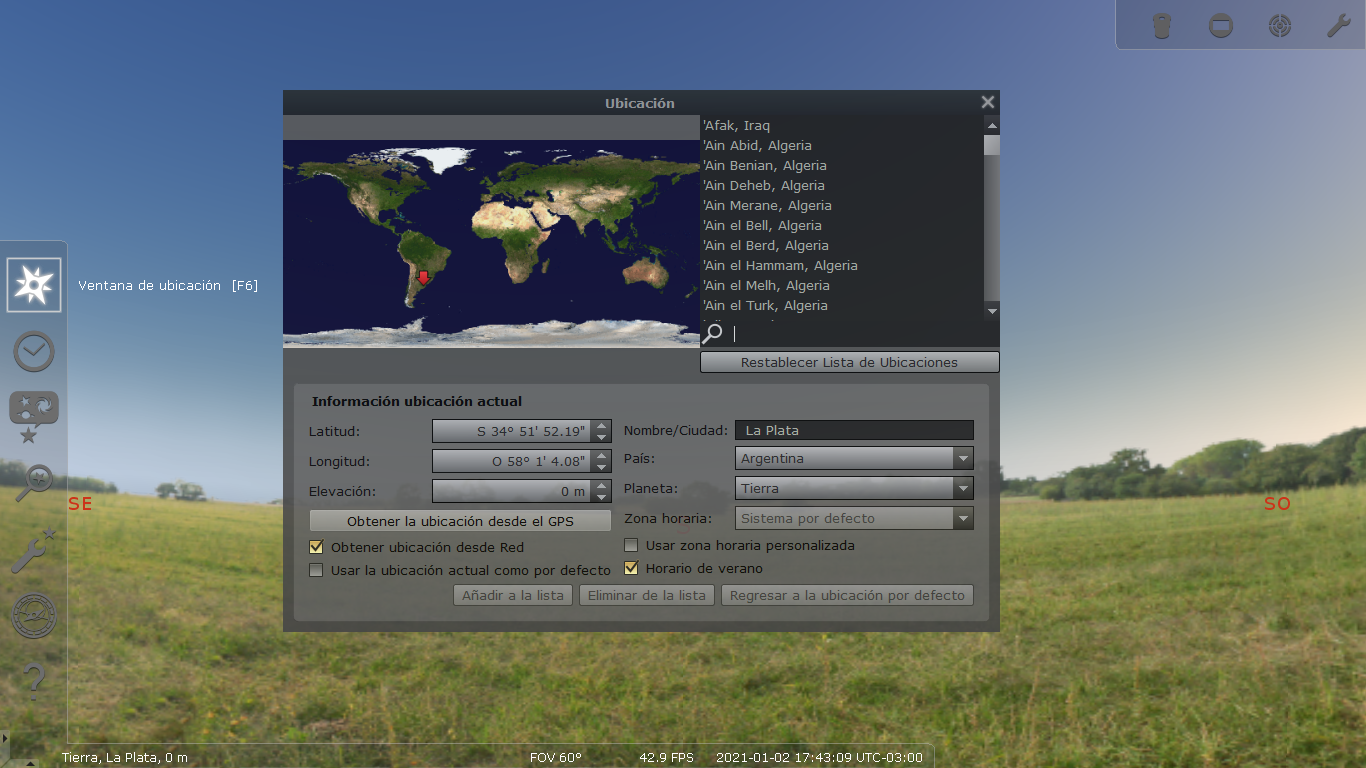
\includegraphics[width=\textwidth]{stel_sel_pos} 
	\caption{configuración de coordenadas locales dentro de stellarium} 
	\label{fig:stell_poss_conf}
\end{figure}

En esa ventana, debe seleccionarse, la latitud, longitud y altitud del lugar en el que se encuentra el telescopio o antena. 

\subsection{Configuración de la red en Stellarium} \label{sub:conf_stellarium_red}


Para poder conectar una PC de la institución, con el dispositivo, debe configurar el puerto(o socket) con el cual se intercambiarán mensajes, y la dirección IP del dispositivo receptor, que será el encargado de mover la antena o telescopio. Para configurar el telescopio, debe dirigirse a configuración, luego presionar en la pestaña pluggins, y en la parte izquierda seleccionar ``control del telescopio''. A continuación se deja la imagen de este proceso: 
 
\begin{figure}[h]
	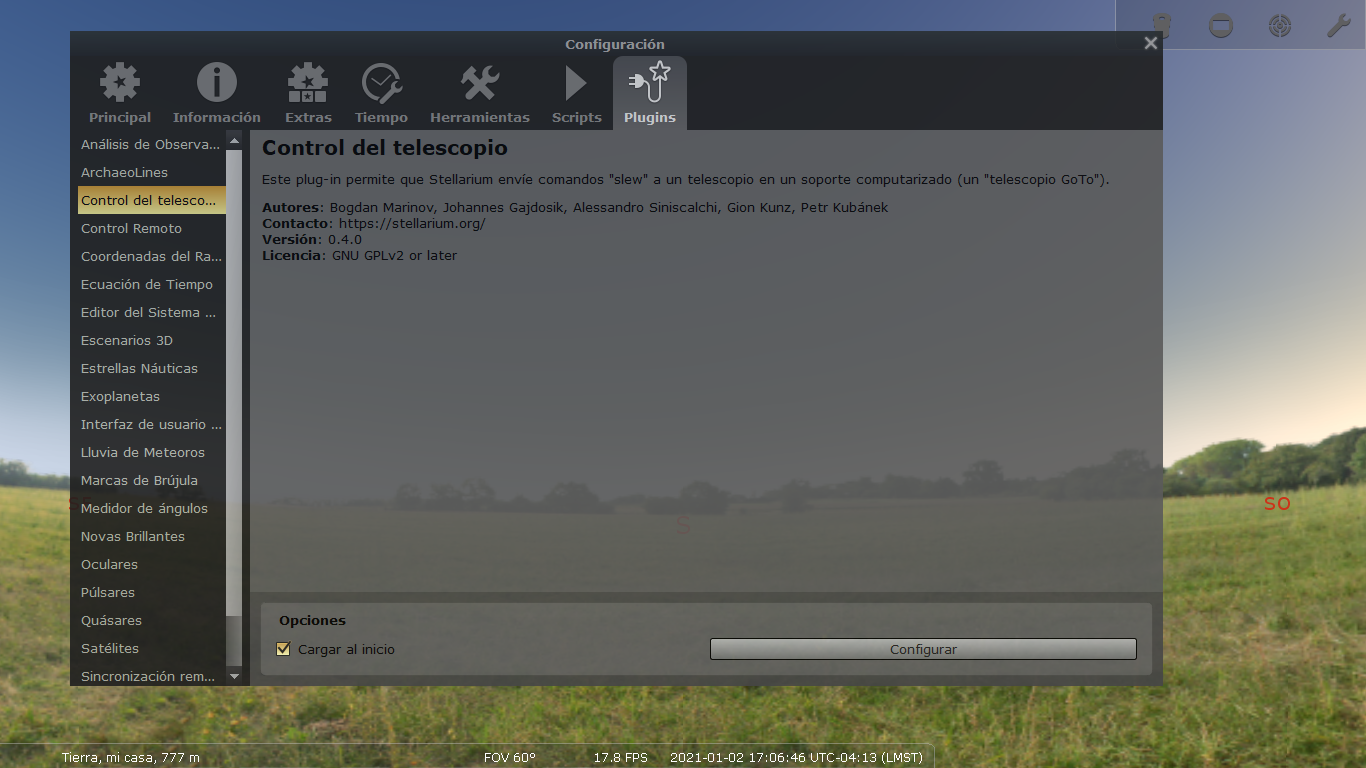
\includegraphics[width=\textwidth]{conf_tel_red1} 
	\caption{configuración de coordenadas locales dentro de stellarium} 
	\label{fig:stell_conf_red}
\end{figure}

Una vez, en esta ventana, se debe seleccionar el botón ``configurar'', debajo a la izquierda de esta ventana, y luego, se abre una ventana cómo la que se muestra a continuación. 

\begin{figure}[H]
	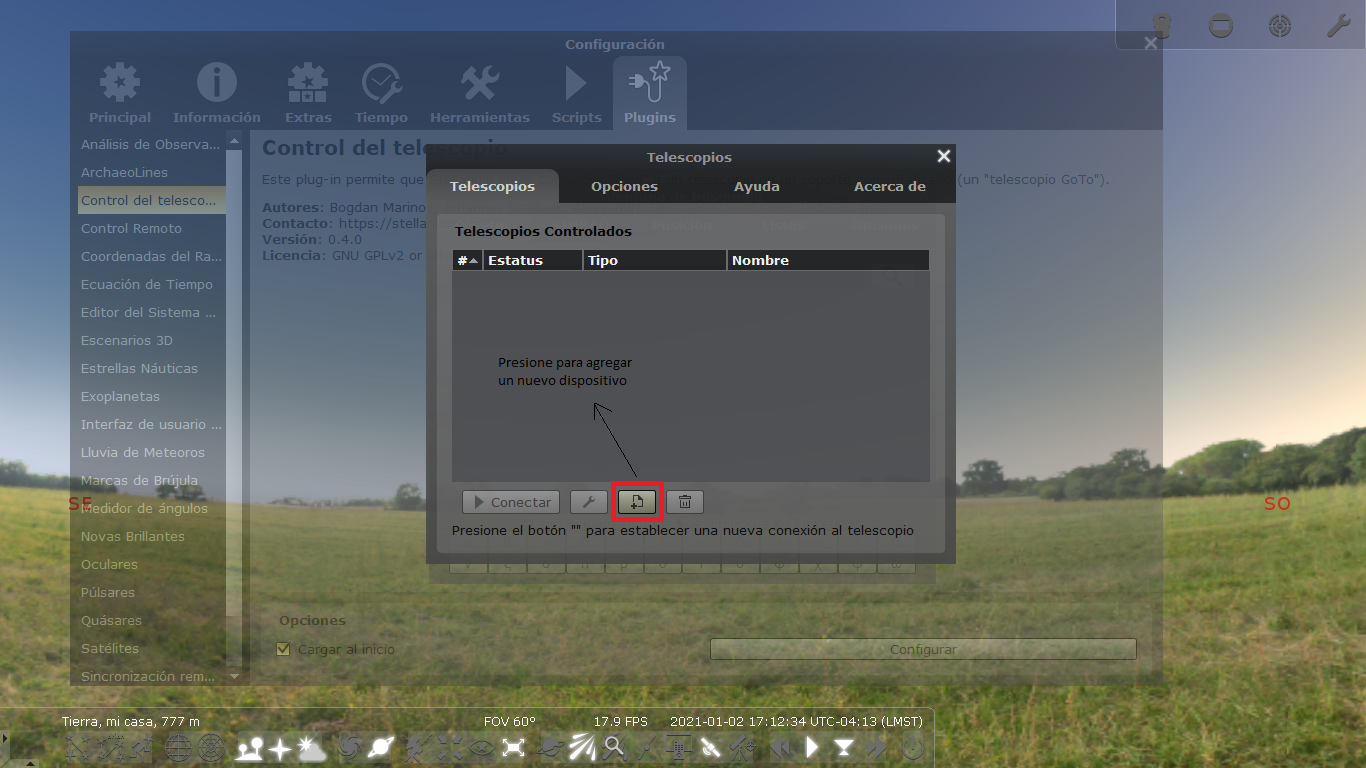
\includegraphics[height=10cm,width=\textwidth]{stell_conf_red_2} 
	\caption{configuración de coordenadas locales dentro de stellarium} 
	\label{fig:stell_conf_red_2}
\end{figure}

Luego, debe presionar donde muestra la imagen anterior para empezar a agregar el primer dispositivo. Se realiza un click sobre el símbolo recuadrado en rojo de la figura anterior, se abre la siguiente ventana, donde deben elegirse los parámetros para configurar el dispositivo hacia cual enviará los datos.
%\begin{wrapfigure}[21]{l}{0.4\textwidth}
\begin{figure}
	\centering
	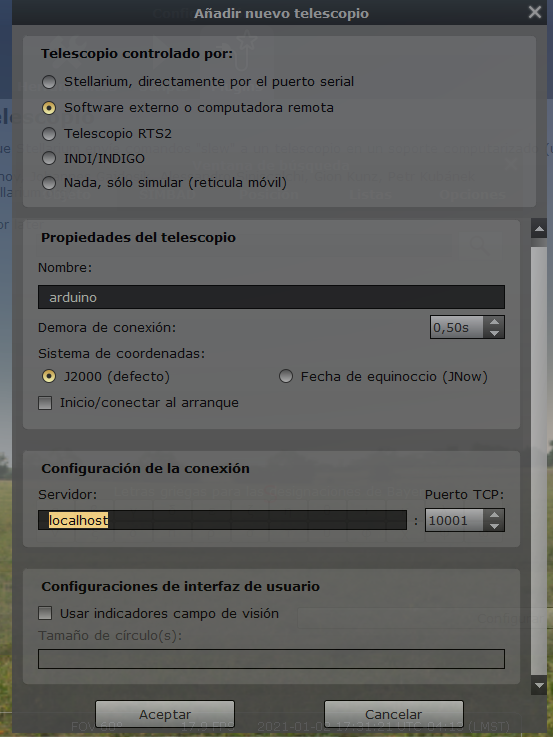
\includegraphics[scale=0.5]{stellarium-024}
	\caption{Ventana de configuración de red del software Stellarium.}
\end{figure} 
Donde dice "localhost",debe introducirse la IP del dispositivo que es capaz de realizar el movimiento de la antena, el nombre, es a elección del usuario, y hay dos tipos de coordenadas: J2000 y fecha de equinoccio. Estas coordenadas están relacionadas con la selección de la referencia para las coordenadas ecuatoriales. Estas se discuten en \ref{cap:sist_cord}. Se elige J2000.

Una vez configurado el dispositivo, queda por intentar entender el protocolo, que éste emplea para comunicarse con los dispositivos. 

\subsection{Protocolo de comunicación Stellarium} \label{sub:comun_stell}
El stellarium, no es capaz de recibir datos en este modo de configuración, pero si es capaz de enviar datos al dispositivo conectado en la red. Este emplea dos números binarios, uno para cada eje. Según su documentación, al configurar un dispositivo, este invoca a un programa denominado ``telescope server'', el cual trabaja sobre TCP/IP. Este, es el que envía las coordenadas al dispositivo. Los mensajes se basan en bytes, donde están agrupados del siguiente modo: 

\begin{itemize}
	\item LENGTH : 2 bytes - Indica la longitud total del mensaje
	\item TIME : 8 bytes. Tiempo UT a partir de 01/01/1970 en microsegundos. Actualmente en desuso 
	\item RA: 4 bytes(sin signo) - ascensión recta: 
	\item DEC : 4 bytes,con signo
	\item status: 4bytes con signo. Si status = 0 -> OK, si status<0 hay algún error.  
\end{itemize}

Cabe destacar, que internet, o las redes, son protocolos big-endian, mientras que el microcontrolador atMEGA328p(arduino UNO) es little-endian. Esto se debe solucionar reordenando los bits de llegada hacia el dispositivo. Además, debe realizar una transformación de coordenadas para poder realizar el apuntamiento de la antena. 


\renewcommand{\chaptername}{Software del microcontrolador}
\graphicspath{{parte_2/soft_micro/}}
\chapter{Software del Microcontrolador} 
\markright{Software del microcontrolador}
\begin{center}
	\begin{tcolorbox}[colback=gray!5!white, %Color del fondo
		colframe=gray!75!black,
		title= \center{\Large{Resumen}} ]
		Se describe todo el proceso realizado,para programar el software para el microcontrolador ATmega328P seleccionado, bajo el entorno arduino, y todas sus librerias. Además, se muestra como deben interconectarse los componentes,y los circuitos correspondientes para realizar las pruebas sobre cada parte del software. Para cada parte del software desarrollado, se han realizado las correspondientes pruebas, y se presentan los resultados en cada sección. Luego una vez, realizadas todas las pruebas, se procede a unir todo el software, y se realiza una prueba final, y se convalidan los resultados.La versión de software presentada en este capítulo, no es la versión final, sino que se agregan más funcionalidades en la siguiente fase(fase 3).   
		 
	\end{tcolorbox}
\end{center}    
\section{Introdución} 
	En este capítulo, se aborda una parte del desarrollo de software de todo el proyecto. La parte restante, se aborda en las fases tres y cuatro respectivamente. El software debe ser capaz de responder a los requerimientos planteados en la tabla \ref{tab:requerimientos}. En esta parte del trabajo, dividimos la programación en varias etapas:  	
	\begin{enumerate}
		\item Control de posición
		\item Autocalibración
		\item Scheduler o planificación 
		\item Conexión del dispositivo a la red. Conectar con Gpredict y stellarium
	\end{enumerate}
	Una vez resueltos, todos los puntos anteriores, se pasa a unir todo el código desarrollado a lo largo de las presentes secciones de este capítulo. Luego, se deja comentado dentro del código aquellas partes que se desarrollen mas adelante a lo largo de este texto. La parte que resta es la transformación de coordenadas, de coordenadas ecuatoriales a coordenadas locales horizontales.  El código en su versión final se muestra en el apéndice.   

\section{Diagrama del sistema} 

En base a los componentes seleccionados, en el capítulo \ref{cap:cap3_sel_hw}, estos deben interconectarse entre si, mediante sus protocolos de comunicación. El sistema de control, se compone del  diagrama en bloques mostrado en la figura \ref{fig:sistema_general}.  
\begin{figure}[ht]
	\centering 
	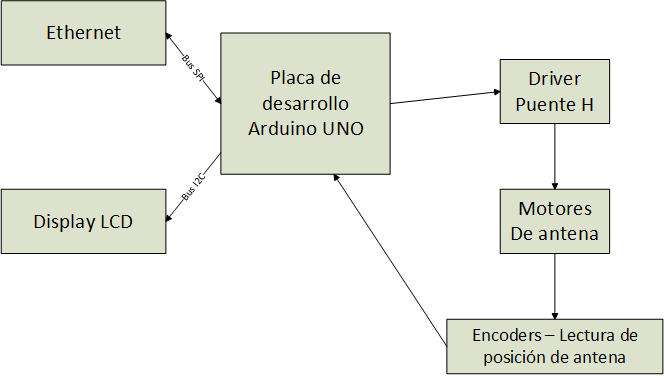
\includegraphics{sistema_general} 
	\caption{Diagrama general del sistema de control} 
	\label{fig:sistema_general}
\end{figure}

Este diagrama en bloques muestra cual es el protocolo de comunicación utilizado por cada dispositivo. La conexión entre el bus SPI soportada por el microcontrolador y el chip ethernet, es el modo 0(ver apéndice \ref{AP:protSerial}), y la conexión con el display es mediante el protocolo SPI(descripto en el apéndice \ref{AP:protSerial}). El bloque de drivers de motores, son dos controladores de motores, y dos encoders, pero se ha puesto una única caja, ya que el sistema de control es el mismo en ambos motores. 

\section{Esquema eléctrico de los componentes}
El lenguaje de programación del entorno arduino es C/C++, y se desarrolla una parte en C y otra parte en C++. El software, debe comunicarse con el display LCD(ver figura \ref{fig:LCD_r}) mediante el protocolo I2C. Este protocolo esta descripto en el apéndice \ref{AP:protSerial}, y con el chip W5100(ver figura \ref{fig:chip_ethernet}) mediante el protocolo SPI(ver apéndice \ref{AP:protSerial}). Por ende, antes de empezar a realizar cualquier tipo de programación, se deben conectar los componentes entre si, para poder realizar la programación, y las pruebas. No se ha utilizado ningún simulador, ya que se disponen de los materiales y componentes, e instrumental necesario para realizar la medición sobre los elementos directamente.  

Antes, de realizar cualquier conexión, se realiza un análisis de los pines disponibles en la placa de desarrollo Arduino Uno, para realizar el desarrollo sin cambiar los pines físicos a lo largo de este trabajo. En primer lugar, se consideran los pines que deben ser utilizados para conectar el chip ethernet. Este debe poseer cinco pines, de los cuales, tres son obligatorios, y no pueden cambiarse desde el software, ya que utiliza el puerto SPI físico del microcontrolador que esta en la placa, estos son los pines 11,12 y 13 respectivamente. El pin de Slave Select, y reset, pueden elegirse indistintamente usando cualquier puerto digital. La conexión del LCD, requiere de comunicación I2C, el cual utiliza dos pines de la placa de desarrollo. Estos pines son los llamados A4 y A5 dentro de la placa.Además, de estos, se requiere cuatro pines adicionales, para controlar el sentido de giro de cada motor(dos pines para cada motor). Estos, deben poseer modulación por ancho de pulso, para poder realizar un control de velocidad en proximos desarrollos de este dispositivo. En este informe, solo se realizará un control de tipo ON/OFF. Los pines disponibles que poseen modulación de ancho de pulso son los pines 9-10, 5 y 6. Luego de estos pines, se deben seleccionar dos pines adicionales, para poder medir la posición angular de la antena,de estos pines se eligen los pines A0 y A1 respectivamente. A continuación, se deja la imagen de cuales son aquellos puertos que se han seleccionado.   

\begin{figure}[H]
	\centering
	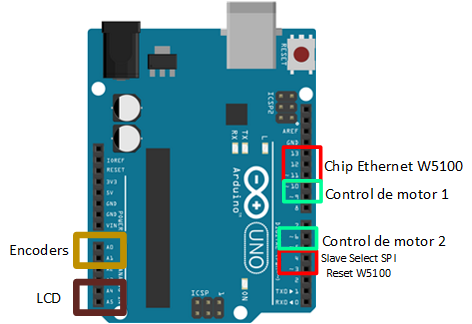
\includegraphics{pines_ard_uno}
	\caption{Pines seleccionados sobre la placa de desarrollo arduino UNO para realizar el prototipo}
	\label{fig:pin_select_ard_uno}
\end{figure}


Una vez, definidos los puertos a utilizar, se deben conectar los componentes a la placa de desarrollo. Esta conexión, se realiza usando cables denominados ''dupont''en una protoboard. 
Para saber como se deben conectar el display LCD y el ethernet Shield W5100, se deben conocer su disposición de pines,o en lenguaje de la jerga electrónica, se debe conocer el "pinout" de cada componente. La explicación de cada pin disponible de cada dispositivo,se muestra en el apéndice \ref{AP:protSerial}. Se muestra el pinout  de cada dispositivo en la figura \ref{fig:pinoutlcdeth}: 

\setlength{\textwidth}{190mm}

\begin{figure}[ht]
%	\centering
%	\hspace{-20mm}
	\begin{subfigure}{0.5\textwidth}
		\centering	
		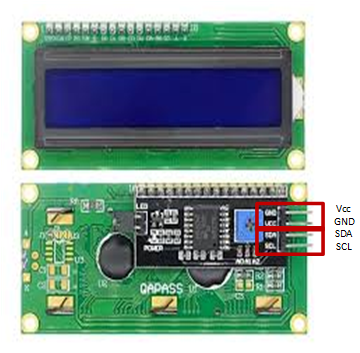
\includegraphics[height=6.3cm]{pinout LCD}
		\caption{Pinout Display LCD }		
	\end{subfigure}
	\hspace{-30mm}
	\begin{subfigure}{0.5\textwidth}		
		\centering
		 
		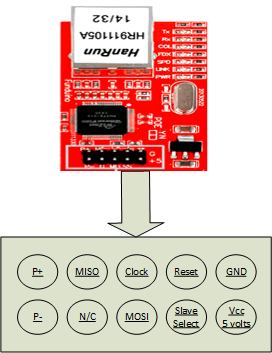
\includegraphics[height=6.3cm]{pinoutW5100}
		\caption{Pinout chip ethernet W5100}	
	\end{subfigure}
	
	\caption{Pinout de ambos componentes, para poder realizar la conexión con la placa de desarrollo de Arduino Uno}
	\label{fig:pinoutlcdeth}
\end{figure}
\setlength{\textwidth}{150mm}

  
Para realizar las conexiones, revisando el diagrama de conexiones dentro del apéndice \ref{AP:protSerial}, se deben conocer cuales son los pines que corresponden a las señales SPI e I2C dentro de la placa de desarrollo. Observando el manual y la hoja de datos, obtenemos que los pines de la placa de desarrollo son los siguientes: 
\begin{itemize}
	\item Chip W5100 
	\begin{itemize}
		\item Pin 13  SCK 
		\item Pin 12  MISO 
		\item Pin 11  MOSI 
		\item Pin 4   Slave Select(SS)
		\item Pin 3   Reset 	
	\end{itemize}
	\item Display LCD   
	\begin{itemize} 
		\item Pin A5  SCL
		\item Pin A4  SDA
	\end{itemize}  
\end{itemize}  

Por último, ya que no se dispone de la conexión al motor aún, se prueban conectando en los pines A1 y A0, dos potenciómetros,de 10Kohms cada uno, ya que cada motor tiene adosado un potenciometro que es utilizado como encoder. Para conocer si el sentido de giro es correcto, en los pines 5,6,9 y 10, se conecta una resistencia y un led,estos led tiene por finalidad, mostrar si el motor gira en sentido correcto, pero estos no se muestran en el esquemático. El esquema de conexiones se muestra en la figura \ref{fig:esq_completo}. 

A continuación se deja una imagen del armado del circuito en una protoboard, en ella, se incluyen las resistencias y diodos led que no se encuentran en la imagen \ref{fig:esq_completo}. 

\begin{figure}[H]
	\centering
	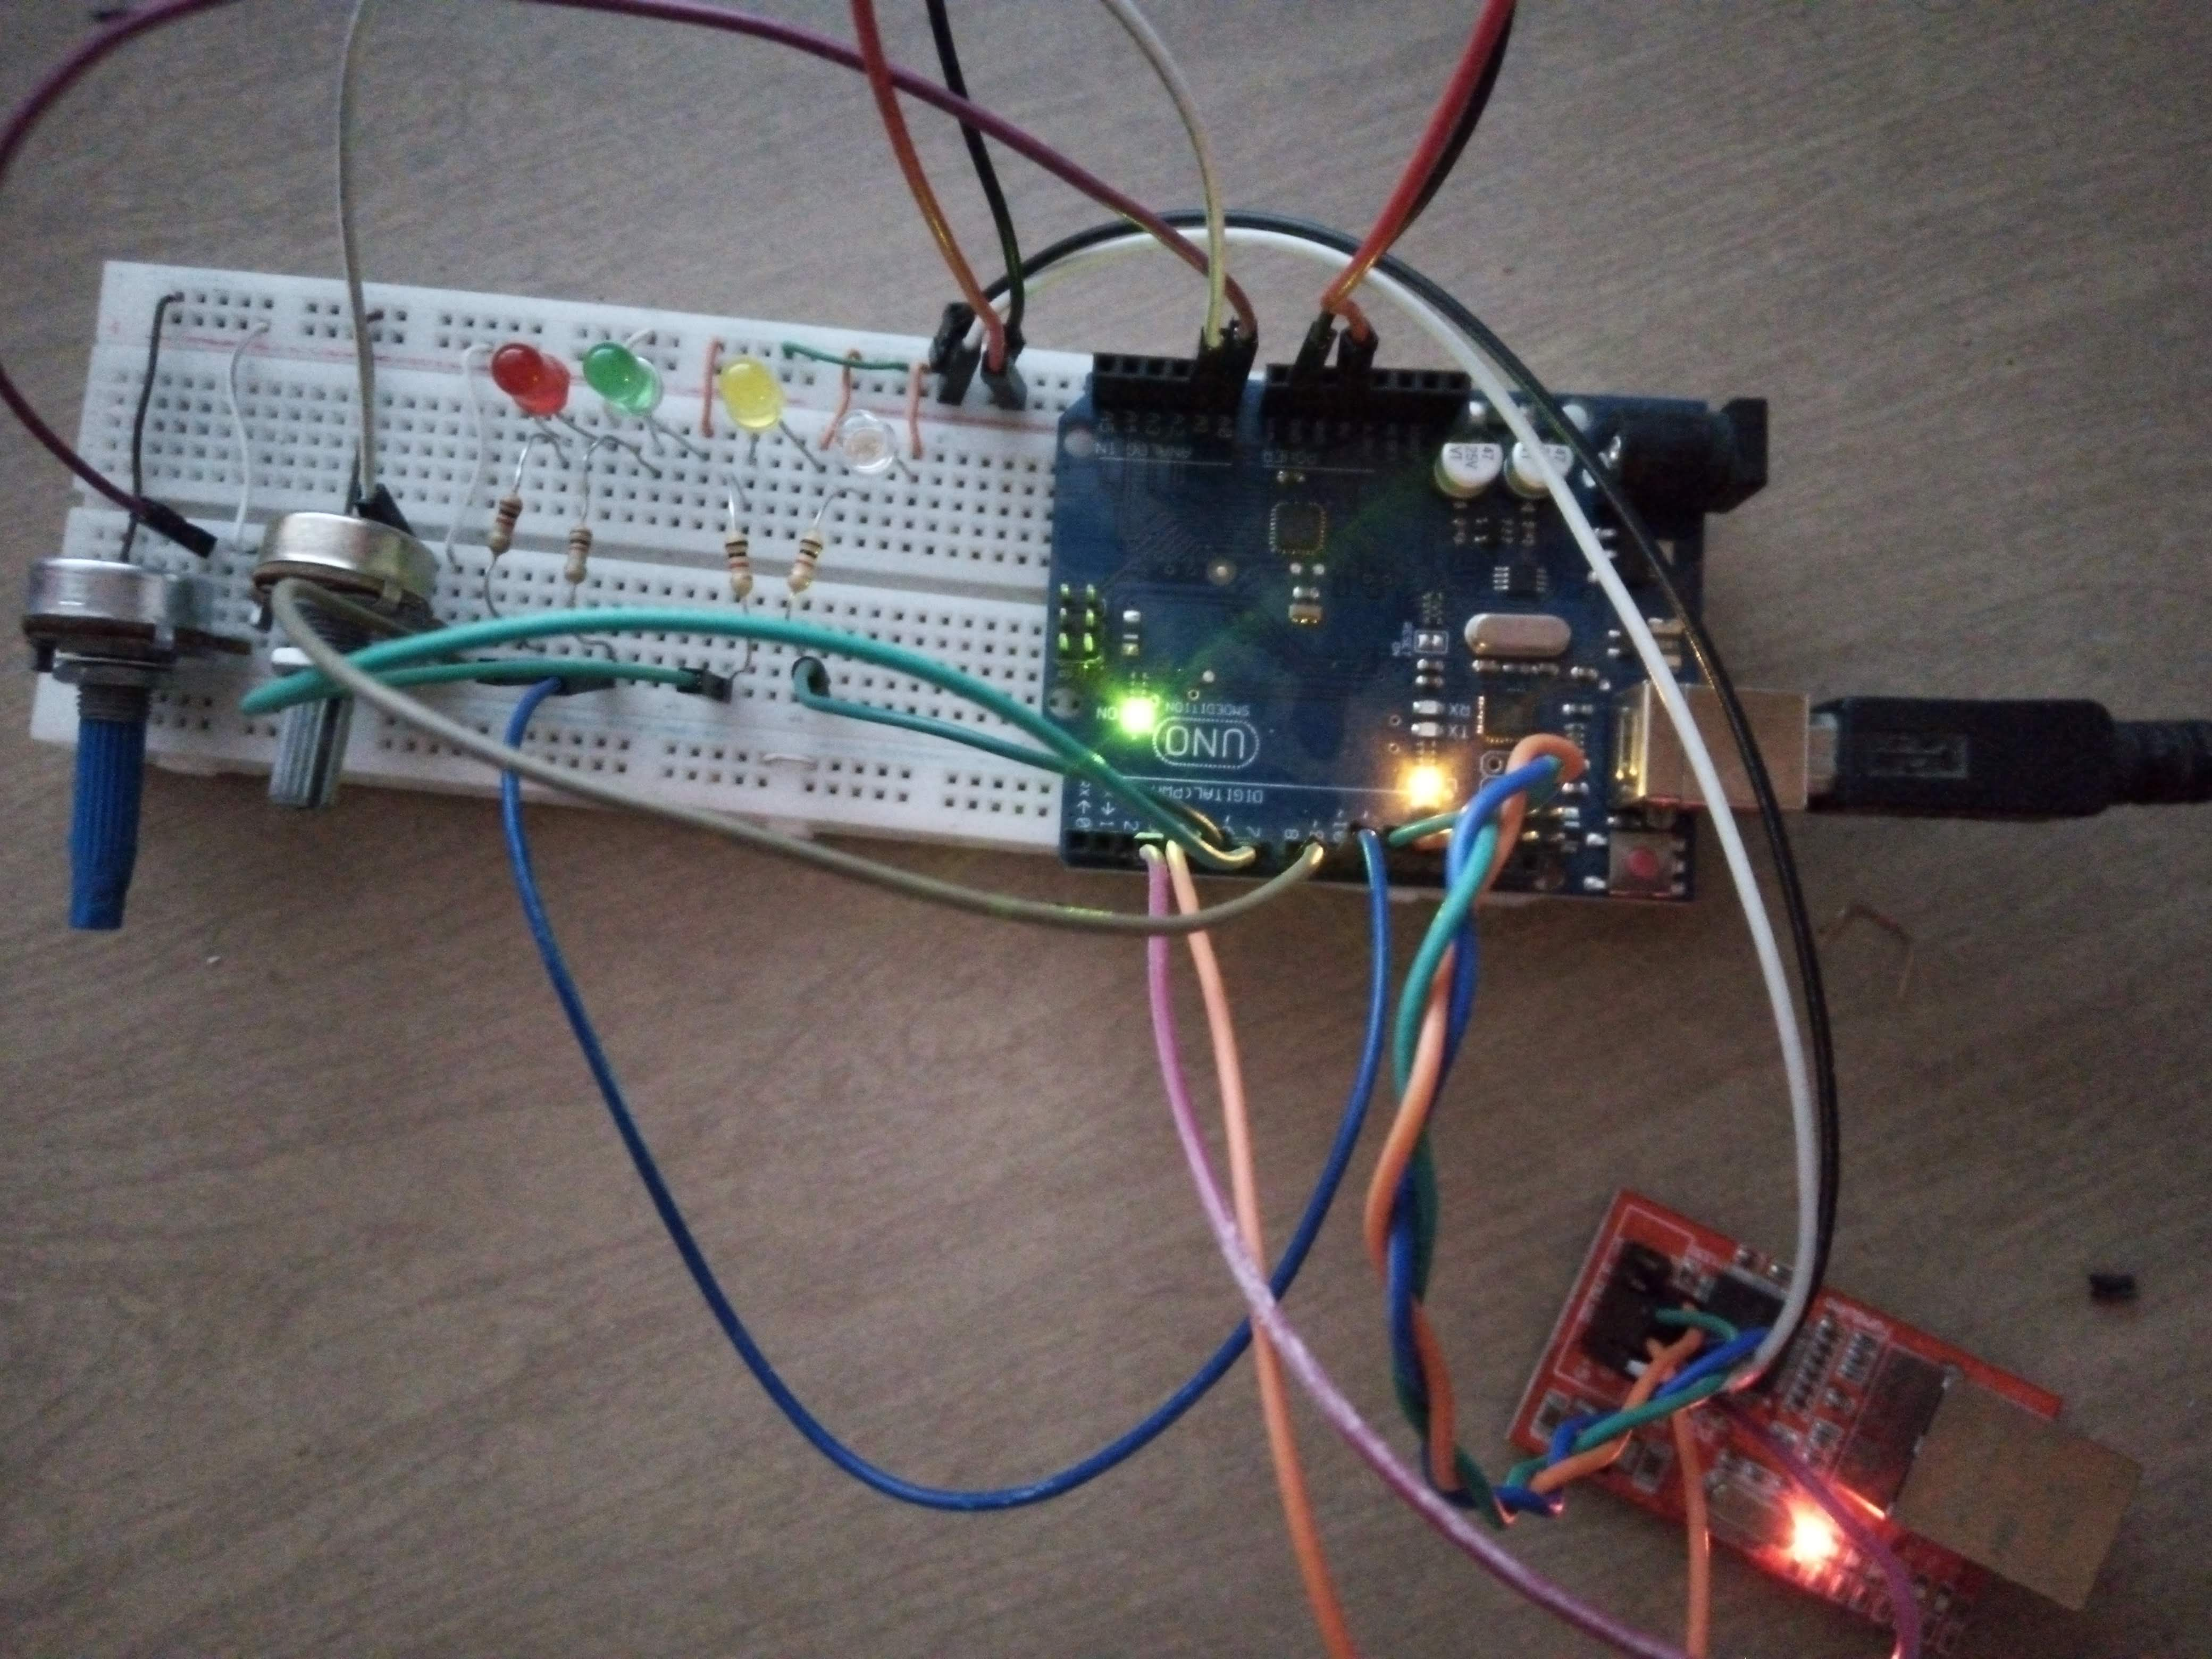
\includegraphics[scale=0.08]{protoboard_1}
	\caption{Imagén del protoboard armado para realizar las primeras pruebas con el software.}
	\label{fig:proto_1}
\end{figure}

\begin{figure}[p]
	\centering 
	\includegraphics[angle=90,scale=0.8]{esquemáticoCircuito}
	\caption{Esquema de conexiones entre la placa de desarrollo y los periféricos utilizados} 
	\label{fig:esq_completo} 
\end{figure}

Donde se ha conectado los diodos led y los potenciómetros de la siguiente manera: 
\begin{itemize}
	\label{item:prototipo_leds_pote}
	\item led rojo: puerto 9 
	\item led verde: puerto 10 
	\item led amarillo: puerto 6 
	\item led azul(el led transparente de la imagen): puerto 5 
	\item potenciometro azul: puerto A0 
	\item potenciometro gris: puerto A1 
	
\end{itemize}


\section{Diagrama general del software}

El software, debe cumplir los requerimientos presentados en el capítulo inicial del presente documento. En principio, deberia tener la capacidad de realizar la autocalibración, al inicio de su programa. Por otro lado, en caso  de que no se este siguiendo ningún satélite o estrella, debería tener la capacidad de volver a la posición de equilibrio de la antena. Esta posición de equilibrio se denomina cenit. 

Cada uno de los motores de la antena, posee adosado un potenciometro, que gira con el motor, esto funciona como un sistema de encoders, para medir la posición angular en base a la tensión. Esta tensión, se mide sobre los pines A0 y A1 de la placa de desarrollo principal. Esta medida, debe actuar sobre los pines 5 y 6 para un eje, y sobre los pines 10 y 9 para el otro eje. Además, debe saber el sentido de giro al prender el led 5 y 6, o 10 y 9. El sentido de giro debe obtenerse de la función de autocalibración.  

El sistema de control, es del tipo ON/OFF, el cual mide la posición y apaga el motor cuando llega a la posición indicada. Son dos controles independientes para cada motor. El estado de apagado, es equivalente a ponera a nivel bajo los puertos 5 y 6, o 9 y 10, según  de que eje se trate. Esta posición a la que debe moverse la antena, viene dada a través de la red, a partir de los programas presentados en el capítulo anterior. 

Además, el software debe informar en todo momento al usuario de su estado (medida angular en ambos ejes, si esta en el cenit, debe escribir la palabra cenit),y la dirección IP asignada por la red, por medio del display LCD.  

Por lo expuesto en los parrafos anteriores de la presente sección, debe realizarse un sistema temporizado, que lea los puertos analógicos A0 y A1, y realizar una acción de control en base a su valor. La acción de control es encender el/los motores en un determinado sentido de giro, y apagarlo cuando llegue a esta. Además, en caso que no este realizando ningún seguimiento, se debe verificar que la antena se encuentre en el cenit. Esto debe realizarse, ya que podrian existir vientos, y/o condiciones climáticas adversas que puedan mover la antena de su posición de equilibrio(el cenit). 


Por lo expuesto en parrafos anteriores, se desarrolla el diagrama de software en la figura  \ref{fig:software_diagrama_general}. En este diagrama, se muestra el software desarrollado en el microcontrolador, y como actuan los distintos puertos del microcontrolador con el hardware. El driver de cada motor, en la figura, se realiza en la fase 4, y es un diseño de hardware. Los encoders 1 y 2 respectivamente, son potenciómetros adosados al eje de cada motor. Estos potenciómetros son de 10Kohms cada uno. Las coordenadas angulares, se denominan angulo de azimut y altura respectivamnte, en astronomía de posición, y por eso se le dió ese nombre. En el capítulo \ref{cap:sist_cord} se tiene una descripción mas detallada de este tipo de coordenadas. 

En la figura se observan dos recuadros, uno denominado "POLLING", y otro denominado "ISR - Esquema de tiempos". El cuadro de POLLING indica que el puerto SPI se mira todo el tiempo, para conocer si existe uno de los programas de la PC(Gpredict, o Stellarium) quiere realizar un movimiento sobre la antena. 


\begin{figure}[ht!]
	\raggedleft
	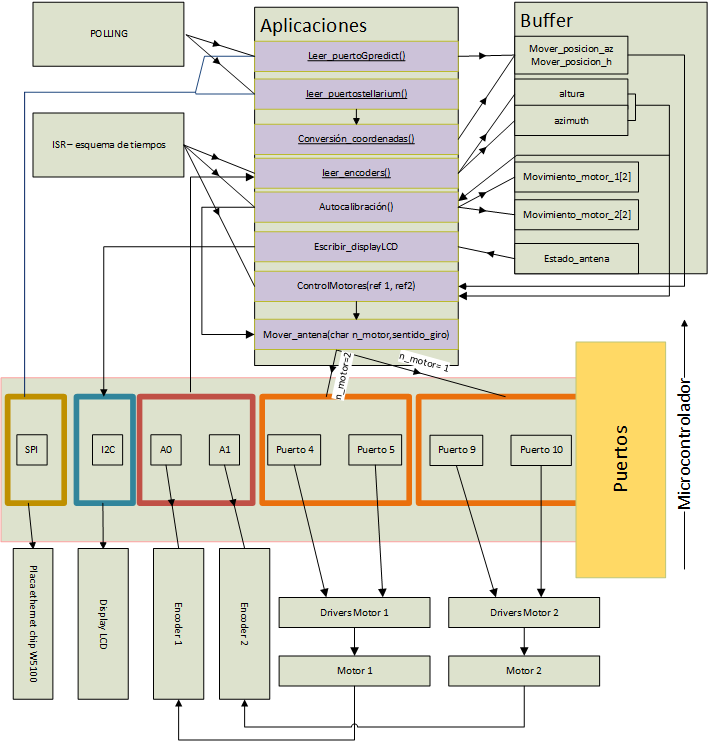
\includegraphics[width=\linewidth]{software_diagrama_general}
	\caption{Diagrama general con las partes de software y hardware}
	\label{fig:software_diagrama_general}
\end{figure}


\vspace{20mm}

El cuadro donde dice "Buffer", son las variables globales que interactuan con las funciones de el programa. Estas variables globales son: 
\begin{itemize}
	\item mover\_posicion\_az y mover\_posicion\_h: referencia para el control de posición, obtenida a travès de los programas Gpredict o Stellarium.  
	\item altura:Posición del ángulo de altura de la antena. 
	\item azimuth:Posición del ángulo de azimuth de la antena
	\item movimiento\_motor\_1$[2]$  y movimiento\_motor\_2$[2]$: en esta se guarda el sentido de giro de cada motor. Dado, que se requieren dos pines para controlar el sentido del motor, y el software debe guardar el sentido de giro, al encender un puerto u otro, estos se guardan en esta variable de tipo vector, siendo: 
		\begin{itemize}
			\item movimiento\_motor\_1$[0]$: Guarda el pin correspondiente al sentido de giro de azimuth, sentido Oeste - Este 
			\item movimiento\_ motor\_1$[1]$ : idem, salvo que el sentido es contrario.  
			\item movimiento\_motor\_2$[0]$: Guarda el puerto correspondiente al sentido de giro desde el plano del suelo hasta llegar a 90° respecto a este. 
			\item movimiento\_motor\_2$[1]$ : Idem, pero guarda el puerto correspondiente al sentido contrario. (a 90° respecto del suelo, hacia el plano del suelo). 			
		\end{itemize}
	
\end{itemize}  



En este diagrama, se han puesto las funciones principales. Cada función, se compone de distintas variables que sirven de soporte al programa en general. Estas no se han graficado en el diagrama de la figura \ref{fig:software_diagrama_general}. Estas funciones,que sirven de soporte a cada función, se muestran a lo largo del presente capítulo. 


%
%\setlength{\textheight}{260mm}
%\setlength{\textheight}{220mm}

El orden del trabajo sobre el software es primero realizar la función de autocalibración. La función de autocalibración, implica que debe llamar a la función mover\_antena(n\_motor,sentido\_giro). En esta sección, se desarrollan ambas funciones. Una vez obtenida y realizada las pruebas sobre la función de autocalibración, se procede a realizar el sistema de control. Esto debe realizarse de esta manera, ya que si no estan calibrados los sentidos de giro del motor, el control no sabra de que forma actuar sobre ellos. Después se continúa con la lectura de los programas Gpredict y Stellarium respectivamente. Luego de esto, se realiza el esquema de polling y el esquema de tiempos o planificación. En la jerga de programación, se denomina "programación por scheduler". Luego en la siguiente fase(fase 3), se desarrolla la teoria de coordenadas, y se implementa la función de transformación de coordenadas. La función que escribe en el display, se desarrolla en la parte final del presente capítulo. 



% diagrama de software 




%
\section{Función de autocalibración}
Esta función, es la primera función a desarrollar. Se supone que el lector posee conocimientos basicos de programación en C/C++, y como debe preparar el entorno para el desarrollo. El entorno elegido es visual Studio Code con el pluggin de PlatformIO. En el apéndice se encuentra como instalarlo y empezar a utilizarlo. 

Antes de realizar la programación, se realiza un archivo, denominado "pinout\_ard\_uno.h", el cual tendrá todas las definiciones de puertos, mostrada en la figura \ref{fig:pin_select_ard_uno}. El archivo contiene las sentencias mostradas en el código \ref{cod:pinout_ard_uno.h}: 


\begin{listing}[ht]

	\begin{minted}[linenos=true,frame=single,highlightcolor = black ,highlightlines={19-20}]{C++}
/**** PINES PARA EL CONTROL DE LOS MOTORES  ***/
		
// motor de cenit 
#define MOTOR_1_S1  5
#define MOTOR_1_S2  6
// motor de azimuth 
#define MOTOR_2_S1  9 
#define MOTOR_2_S2  10 
		
/* PINES ETHERNET */
 #define PINSS 4
 #define PINRESET 3  
		
/* PINES ENCODERS*/
 #define PINENCODERAZ A0   //MEDIDA DE AZIMUTH 
 #define PINENCODERH  A1   //MEDIDA DE ALTURA 
		
// flags para utilizar depuracioon 
 #define TIMER_CLOCKS 0 // para depurar las aplicaciones sin timers establecidos  
 #define DEBUG  1      // depuración de aplicaciones usando puerto serie .  
		
\end{minted}
	\vspace{-5mm}
	\caption{definición de los puertos del microcontrolador. El nombre del archivo es "pinout\_ard\_uno.h".}
	\label{cod:pinout_ard_uno.h} 
\end{listing}
Donde las variables \mintinline{C++}{TIMERS_CLOCKS} y \mintinline{C++}{DEBUG}(resaltadas en la \ref{cod:pinout_ard_uno.h}) son utilizados para realizar compilaciones condicionales, mientras se desarrolla.Las compilaciones condicionales se explican en el apéndice \ref{ap:ard_uno_env} .
 
Una vez definido los puertos, para realizar esta función de autocalibración, debe conocer cual es el sentido de giro, al poner en estado alto, el pin 10 y 9, o 6 y 5, y guardar este resultado. Para realizar esto, cada motor que mueve la antena, tiene adosado un potenciometro. El giro de este potenciometro, nos indica la medida angular. Un potenciometro, consta de tres pines, donde uno esta conectado a la fuente de tension, otro a tierra, y el del medio se dirige al pin A0 o A1 del microcontrolador. Al girar este, cambia su resistencia entre el punto medio y tierra, cambiando al tensión, y esta tensión es la que se mide desde el microcontrolador. En la figura
\ref{fig:pot} se encuentra la imagen de un potenciometro. 

%\setlength{\textheight}{260mm} 

\begin{SCfigure}[50][h]
	\centering
%	\vspace{-20mm}
	\caption{Vista de un potenciometro, y sus respectivas conexiones de tensión, y con el microcontrolador.}	
	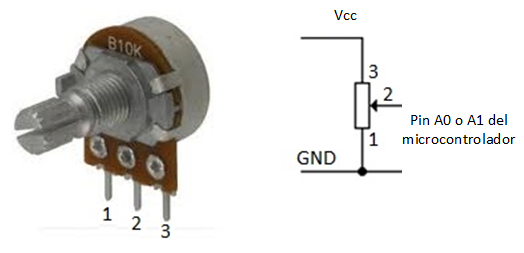
\includegraphics[height=3.2cm]{pote}
%	\begin{minipage}
	\label{fig:pot}	
%	\end{minipage}
	%\caption{Vista de un potenciometro, y sus respectivas conexiones de tensión, y con el microcontrolador.}	
\end{SCfigure}
\vspace{30mm}

%\setlength{\textheight}{240mm}

Como se observa en la figura(\ref{fig:pot}), la salida de tensión(pin 2 de la figura), con respecto a GND, cambía, cuando se gira el eje del potenciometro. Esta tensión, es la que se mide el conversor analógico digital del microcontrolador atMEGA328p. El conversor analógico-digital se explica en el apendice \ref{ap:ard_uno_env}   

Para poder realizar la autocalibración, se debe definir, si la tensión en un extremo de la posición de la antena, es maxima, y en el otro extremo es mínima. Con esto, el software se dará cuenta, en que sentido se esta moviendo la antena(esta definición debe realizarse en ambos ejes de la antena). El software se dará cuenta, ya que podra revisar si la tensión de entrada, esta aumentando o disminuyendo, y en base a esto, se asignan los sentidos de giro dentro de las variables movimiento\_motor\_1 y movimiento\_motor\_2. 

Los sentidos de giro de máxima y mínima tensión, se deben definir sobre los ejes de la antena. Estos ejes se mueven como muestra la figura \ref{fig:mov_antena}. 

\begin{figure}[ht]
	\centering
	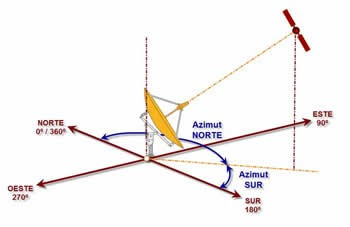
\includegraphics[height=5cm]{mov_antena}
	\caption{Movimientos que puede realizar la antena usando sus dos motores.}
	\label{fig:mov_antena}	
\end{figure}


La antena, solo tiene movilidad ESTE- OESTE, apuntando hacia el sur. Por este motivo, definimos que la mínima tensión esta dada en el oeste, y la máxima tension en el este,donde se define 0° en el OESTE, y 180° en el ESTE, en sentido antihorario. En sentido del eje horizontal, definimos la mínima tensión, a 90° respecto al piso, y máxima tensión cuando la antena se encuentre a 0° del plano del suelo. Utilizamos esta convención para realizar la medida sobre el ángulo de altura. Además, debe definirse a que eje del movimiento de la antena, corresponde a cada puerto. Siguiendo el código \ref{cod:pinout_ard_uno.h}, se observa que se define el puerto A0 para el ángulo azimutal y el puerto A1, para el ángulo de altura. Las definiciones de tensión y puertos, se resumen en la siguiente tabla: 
\begin{table}[ht]
	\centering 
	\begin{tabular}{|c|c|c|c|}
		\hline
		Eje & Puerto & punto de máxima tensión & punto de mínima tensión\\ 
		\hline
		azimuth &A0 & Este(180º) & Oeste(0º) 	 \\    
		\hline
		altura  &A1 &  paralelo al suelo& 90º respecto al suelo  \\
		\hline
	\end{tabular}
	\caption{Definición de sistema de coordenadas para la antena}
	\label{tab:def_sist_coord}
\end{table}

Por lo expuesto en los parrafos anteriores, la función de autocalibración debe realizar los siguientes pasos: 

\begin{enumerate}
	\item Poner en alto, los pines 5 y 10 respectivamente, y los pines 6 y 9 en bajo  
	\item Tomar el dato de los puertos analógicos-digitales de los pines A0 y A1. 
	\item Guardar este dato, y compararlo con el próximo. Si es mayor, gira en un sentido u otro. Esto debe realizarse para ambos ejes. 
	\item Esperar que llegue al final de su recorrido la antena(ambos ejes). Luego guarda el valor final. Se da cuenta, que llega a su recorrido final, si las últimas tres muestras son identicas
   \item invertir los pines del paso 1, y realizar los pasos 2 y 3 respectivamente, pero ahora, guarda el segundo valor final. Luego se comparan ambos, y el programa, puede saber en que sentido giraron los motores. Con estos valores, se calcula la resolución angular del apuntador. 
\end{enumerate}

Esta función,se debe realizar al iniciar el equipo.  

Antes, de realizar la función de autocalibración, se ha realizado la función, que lea desde los potenciómetros la posición actual, y las guarde en las variables azimuth y altura, respectivamente. Para esta función, se han creado dos archivos: uno denominado ``lectura\_encoders.cpp'' y otro denominado "lectura\_encoders.p". Este último, tiene los prototipos de las funciones compartidas, que deben ser accedidas desde otra parte del código. El archivo ``lectura\_encoders.cpp", tiene las funciones propias de su funcionamiento, y el comportamiento de las funciones definidas en ``lectura\_encoders.h". 
\begin{listing}[ht]
	\begin{minted}[linenos,frame= single]{Arduino}
#include "Arduino.h" 
#include "../pinout_ard_uno.h"
// variables tipo buffer 
int azimuth ; 
int altura ;

extern enum _state_antena 
{
	AUTOCAL ,  
	NO_AUTOCAL, 
} antena ;

void leer_encoders()
{
	azimuth = analogRead(PINENCODERAZ) ; 
	altura  = analogRead(PINENCODERH) ; 
	if (antena==AUTOCAL) 
	{
		return;
	}
	//transformacion de coordenada---> retornar la transformación
}

	\end{minted}
\caption{archivo lectura\_encoders.cpp. }
\label{cod:lectura_encoders.cpp}
\end{listing}

La única función definida en este archivo es \mintinline[style=arduino] {Arduino}
{leer\_encoders()} es devolver el valor leido por el conversor analógico digital, cuando se esta autocalibrando. Esta función se muestra en el código \ref{cod:lectura_encoders.cpp}. Si no se esta autocalibrando, deberá devolver las coordenadas correspondientes. En este caso, esa parte, se va programar en la próxima sección. 

Una vez realizado el proceso de lectura de los encoders por parte del microcontrolador, ahora resta la función de autocalibración.  Esta esta divida en dos archivos, uno denominado ``control\_motores.h'' y ``control\_motores.cpp''. 

Esta función de autocalibración, debe ser capaz de mover los motores, por ende, se crea la funcion \mintinline{Arduino}{mover_antena(char n_motor,sentido)} , donde n\_motor es el motor de azimuth si n\_motor es uno, o el motor de altura si toma el valor 2. Esta variable define el número de motor. Los sentidos, se definen  como 0,1, o 2 respectivamente, siendo: 
\begin{itemize}
	\item sentido = 0 :  Apagar motor 
	\item sentido = 1 :  Encender el puerto  \mintinline[style=arduino]{Arduino}{MOTOR_1_S1}(ver código \ref{cod:pinout_ard_uno.h}, idem para las otras variables mencionadas) en alto y \mintinline{Arduino}{MOTOR_1_S2} en estado bajo si el número de motor es 1, si el número de motor es 2,se definen en alto el puerto  \mintinline{Arduino}{MOTOR_2_S1} y en bajo el puerto 
	\mintinline{Arduino}{MOTOR_2_S2} 
	\item sentido = 2: define los puertos en forma inversa al sentido que los define sentido = 1 
\end{itemize}
 
Una vez, se ha definido la función \mintinline{Arduino}{mover_antena(char n\_motor,char sentido)}, se pasa a realizar la función de autocalibración.  El código de la función de\mintinline{Arduino}{mover_antena(char n\_motor,char sentido)},se observa en el apéndice del presente capìtulo.   

La función de autocalibración, utiliza las funciones \mintinline{Arduino}{leer_encoders} y \mintinline{Arduino}{mover_antena}, y funciones auxilares. Estas funciones son: 

\begin{itemize}
	\item \mintinline{Arduino}{assign_value_autocal()}  
	\item \mintinline{Arduino}{mover_antena(char n_motor, char sentido)}   
	\item \mintinline{Arduino}{function_compare_autocalibracion()}  
	\item \mintinline{Arduino}{assignar_sentidos_motores()}
\end{itemize}

Además, utiliza variables auxiliares. Estas se denominan: 
\begin{itemize}
	\item ult4ad[4]: guarda los ultimos cuatro valores leidos del encoder. En ult4ad[0] y ult4ad[1] guarda los ultimos dos valores del angulo de azimuth, y en ult4ad[2] y ult4ad[3] guarda los dos últimos valores del angulo de altura. 
	\item estado\_autocalibracion[2]: guarda el sentido(1,2, o 0) del motor en el estado actual. El valor de estado\_autocalibracion[0] corresponde al motor de azimut, y el otro al valor de sentido del motor de altura 
	\item calibracion\_encoders[4]: guarda los valores maximos y minimos leidos por los encoders. calibracion\_encoders[0] y calibracion\_encoders[1] corresponden a los valores del encoder correspondiente al ángulo de azimuth. Los otros dos, corresponden al valor del ángulo de altura.   
\end{itemize}

No se mostrará todo código desarrollado para esta función de autocalibración. En su lugar, se da el diagrama de flujo del funcionamiento de esta función en la figura \ref{fig:flujo_autocalibracion}. La función assignar\_sentidos\_motores() se encarga de guardar los sentidos dentro de la variables buffer motor\_asignacion\_1 y motor\_asignacion\_2, según los criterios de la sección anterior. 
\begin{figure}[ht]
	\centering
	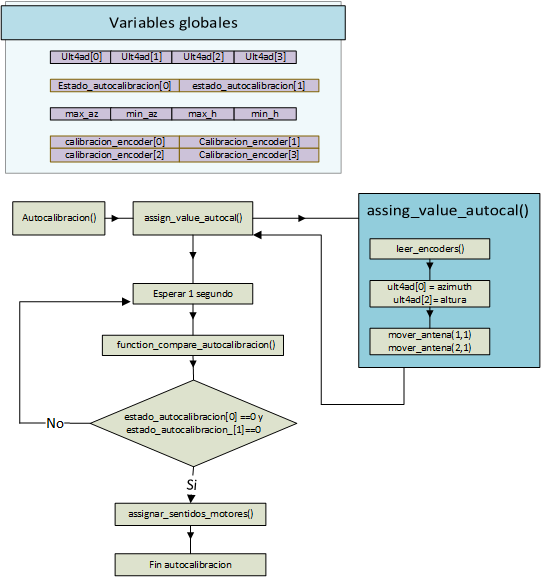
\includegraphics{flujo_autocal} ; 
	\caption{Diagrama de flujo de la función de autocalibración.}
	\label{fig:flujo_autocalibracion}
\end{figure}

La idea del algoritmo es la siguiente: 
\begin{enumerate}
	\item LLamar a la función assign\_value\_autocal(). Esta lee los encoders, y pone el sentido = 1 en ambos motores. 
	\item Luego espera un segundo. signa los valores correspondientes dentro de las variables. Luego le asigna el sentido 1 a cada motor. Además, asigna los valores de calibracion\_encoders[0] y  calibracion\_encoders[1] en uno. 
	\item LLama a la función de comparación function\_compare\_autocalibracion(). Esta función, es la encargada de realizar las comparaciones y cambiar el estado de calibracion\_encoders[0] o calibracion\_encoders[1], cuando cambia por primera vez, se cambia a 2, y la tercera vez, cambia a cero. La comparación debe realizarse cada un segundo, para que la antena, tenga el tiempo suficiente de moverse.  
	\item assignar\_sentidos\_motores(): Toma los valores de calibracion\_encoders, y los compara. En base a eso, asigna los sentidos dentro de las variables asignacion\_motor\_1 y asignacion\_motor\_2 respectivamente. 
\end{enumerate}


La función de comparación, en primer lugar lee los valores actuales de los encoders, y luego los compara con los anteriores para saber si el valor actual es igual al anterior. Luego, borra los valores actuales, y los pasa como valores antiguos, y los compara con los que siguen. Asì, sigue hasta que los últimos dos valores son iguales.

Los códigos de programación,de todas las funciones auxiliares, incluyendo la de autocalibración, se encuentran en el apéndice del presente capítulo. 

Luego, la función de autocalibración,se programó con el código mostrado en \ref{cod:autocalibracion}. 

\begin{listing}[ht]
	\begin{minted}[linenos,frame=single]{Arduino}
void autocalibracion()
{
assign_value_autocal() ;
delay(1000) ; 
function_compare_autocalibracion() ; 
while (estado_autocalibracion[0]!=0 || estado_autocalibracion[1]!= 0)
{
  delay(1000) ;     
  function_compare_autocalibracion() ;             
}
//ASIGNACIÓN DE MOTORES 
assignar_sentidos_motores() ; 
#if DEBUG==1
// depuración por puerto serie . 
Serial.print("calibracion encoders az: ");                   
Serial.print(calibracion_encoders[0]); Serial.print(" ");
Serial.println(calibracion_encoders[1]) ;
Serial.print("calibracion encoders h: ") ;
Serial.print(calibracion_encoders[2]); Serial.print(" ");
Serial.println(calibracion_encoders[3]) ;
Serial.print("movimiento_motor_1: ") ; 
Serial.print(movimiento_motor_1[0],DEC) ; Serial.print(" "); 
Serial.println(movimiento_motor_1[1],DEC) ;
Serial.print("movimiento_motor_2: ");
Serial.print(movimiento_motor_2[0],DEC); 
Serial.print(" ");
Serial.print(movimiento_motor_2[1],DEC); 			

#endif    	
}
\end{minted}
\caption{Código de la función de autocalibración. Esta definido en el archivo "control\_motores.cpp"}
\label{cod:autocalibracion}

\end{listing}

\subsection{resultados de la función de autocalibración}

Para revisar los resultados de la función de autocalibración, se ha definido una bandera de compilación denominada \mintinline{C++}{DEBUG} donde, se van a imprimir los resultados por puerto serie. 

El prototopo armado es el de la figura \ref{fig:proto_1}, y las conexiones del potenciometro y los diodos leds, se encuentran debajo de la imagen.  
%
%Para probar la función, se ponen los potenciómetros, en un extremo, luego en el otro, y luego en el medio. Luego se giran, hacia la derecha, o izquierda, y luego se giran en sentido contrario. Se registran los resultados en el puerto serie, y observando que los diodos leds, se encuentren apagados al finalizar la prueba. Los resultados arrojados por el puerto serie se resumen en la siguiente tabla. 

Para realizar la prueba del programa, se pone el potenciometro en una posición inicial, y luego se gira el potenciometro. Hay tres posiciones iniciales, que empiece en uno de los dos extremos, o que empiece en un punto medio. Si empiezan en un extremo, solo se debería girar una vez hacia el otro extremo. Si empieza en un punto medio, se debe girar dos veces, una para un extremo, y luego hacia el otro extremo. Para realizar esta prueba, dentro del código \ref{cod:pinout_ard_uno.h} se pone la bandera DEBUG en 1, y se utiliza el código mostrado en \ref{cod:autocalibracion}. Este código arroja los resultados por el puerto serie. Estos resultados, se resumen en la tabla \ref{tab:resultados_autocalibracion},donde el sentido viene dado, por los potenciómetros vistos de frente.   

%\renewcommand{\arraystretch}{1.5} 
\begin{table}[ht!]
	\begin{tabular}{|c|c|c|c|c|c|c|}
		\hline 
		\multicolumn{7}{|c|}{motor 1} \\
		\hline 
		\multirow{2}{*}{posición inicial} & 
		\multirow{2}{*}{primer giro} &\multirow{2}{*}{segundo giro} & \multicolumn{2}{l|}{calibracion\_encoders}& \multicolumn{2}{l|}{asignacion\_motor\_1} \\ \cline{4-7} 
		   & & & índice 0 &índice 1 &índice 0 &  índice 1 \\
		 \hline 
	      punto medio & giro derecha & giro izquierda & 1023 & 1 & 1 & 2 \\
	     \hline 
		 punto medio & giro izquierda & giro derecha & 0 & 1018 & 2 & 1 \\
		 \hline 	
		extremo izquierdo & giro derecha & x & 0 & 1007 & 2 & 1 \\
		\hline 
	    extremo derecho & giro izquierda & x & 1023 & 1 & 1 & 2 \\
		\hline 	
		\hline
		
		%\hline 
		\multicolumn{7}{|c|}{motor 2} \\
		\hline 
		
		\multirow{2}{*}{posición inicial} & 
		\multirow{2}{*}{primer giro} &\multirow{2}{*}{segundo giro} & \multicolumn{2}{l|}{calibracion\_encoders}& \multicolumn{2}{l|}{asignacion\_motor\_2} \\ \cline{4-7} 
	%	\hline 
		   & & & índice 2 &índice 3 &índice 0 &  índice 1 \\ 
		\hline 
		 punto medio & giro derecha & giro izquierda & 898 & 1 & 2 & 1  \\
		\hline 
		 punto medio & giro izquierda & giro derecha & 17 & 1023 & 1 &2  \\
		\hline 	
		 extremo izquierdo & giro derecha & x & 0 & 1023 & 1 &2  \\
		\hline 
		 extremo derecho & giro izquierda & x & 1023 & 1 & 2 & 1 \\
		\hline
		\end{tabular}
	\caption{Resultados de la función de autocalibración.}
	\label{tab:resultados_autocalibracion}
\end{table}

Al analizar la tabla anterior, se observa, que la función de autocalibración, responde correctamente para ambos motores. Por ejemplo, la primer fila del motor 1, se empieza del punto medio,con el sentido siendo 1(ver seccion anterior), y se gira el potenciometro hacia la derecha, y guarda el valor leido del conversor A/D:1023 en este caso. Cambia de sentido,con el valor de sentido 2, y se gira el potenciometro hacia el otro extremo. En este caso, el valor leido es 1. Luego, el sentido Oeste - Este es el sentido con valor 1, ya que el primer giro, aumentó la tensión. Luego al invertir los puertos, se gira hacia el otro lado, y se observa, que la tensión disminuye. Esto indica que el sentido de giro es en el sentido este - oeste. Luego el valor guardado del sentido Oeste - Este debe ser 1, y el sentido contrario, debe ser 2. Se analiza de la misma manera los restantes, y se observa que el comportamiento es el esperado. 

Cabe destacar, que el giro de los potenciómetros se ha realizado de forma manual. Los potenciómetros que van a usarse, estan adosado al eje de la antena, y estos realizan el movimiento, a medida que gira el/los motores.  

\section{Control de la posición}
El control de la posición, consta en leer la posición enviada desde el software Gpredict o Stellarium, y mover la antena hacia esa posición. Además, si no recibe, ninguna posición de estos programas, el software, debe ser capaz de regresar a la posición de equilibrio, o denominada cenit. Esta posición es equivalente a 90º en posición azimutal y 90º respecto del suelo. 

Recordando, que cada motor, tiene adosado un potenciometro, que es utilizado como encoder, se procedió a medir el potenciometro. Este potenciometro se encuentra adosado a cada motor, y deben medirse, para conocer la variación de la tensión en función del ángulo. 

Para realizar esta medición, se ha realizado un script en el lenguaje python, que se conecta al microcontrolador,y un programa sobre el microcontrolador. El microcontrolador, envía los datos leidos del potenciometro, y el script, los guarda en un archivo de texto. Ambos programas se encuentran en el anexo del presente capítulo.

Una vez creados ambos programas, sobre el microcontrolador, y sobre la pc(script en python), se conecto el punto medio del potenciometro al microcontrolador, y se realizó el giro del motor con una fuente de laboratorio. Ambos motores, se girán de tal manera que la antena, tenga su recorrido completo en ambos ejes. La tensión de la fuente fue de 24 V. Estos datos, se registrarón cada 1 milisegundo. Los resultados fueron los siguientes: 


\begin{figure}[ht]
    \hspace{-10mm}
	\begin{subfigure}[t]{0.5\textwidth}
		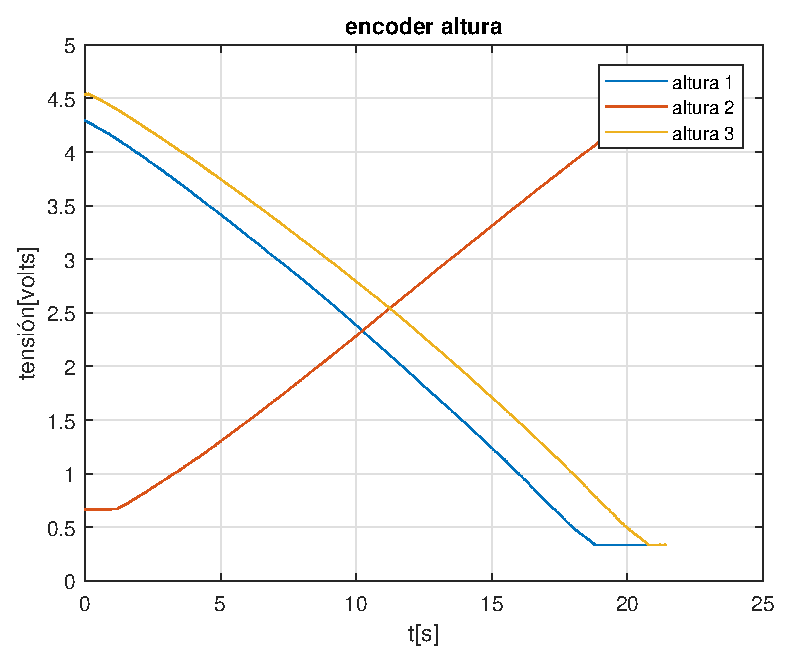
\includegraphics[width=\textwidth,height=6cm]{medidas_cenit} 
		\caption{Encoder de altura} 
		\label{subfig:altura} 
	\end{subfigure}
	\hspace{10mm}	
	\begin{subfigure}[t]{0.5\textwidth}
		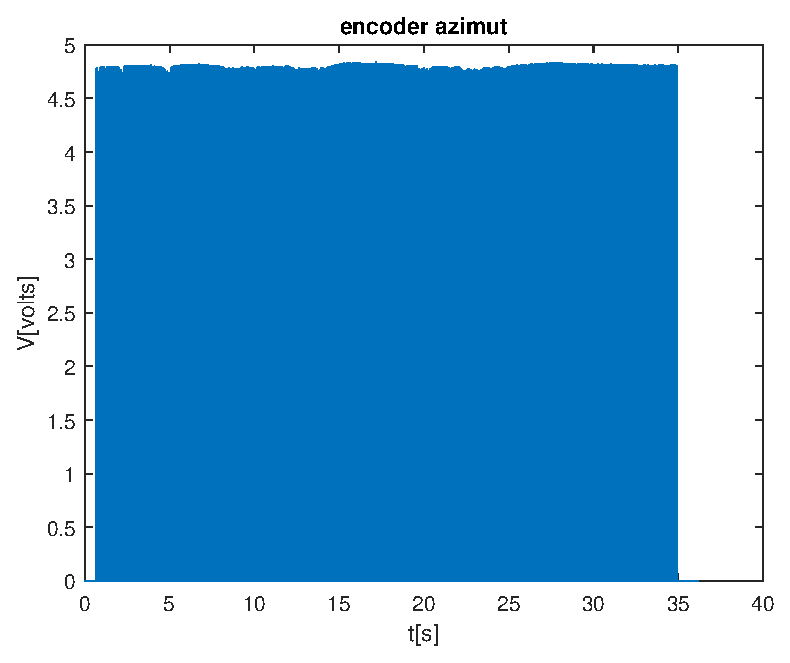
\includegraphics[width=\textwidth,height=6cm]{medidas_azimut}
		\caption{Encoder azimut}  
		\label{subfig:azimut} 
	\end{subfigure}
	\caption{Medidas realizadas sobre los encoders de la antena en función del tiempo.}
\end{figure}


Se observa en el ángulo de altura(ver figura \ref{subfig:altura}), que el potenciometro responde de forma lineal en función del tiempo, mientras que el ángulo de azimuth, utiliza una serie de pulsos para medir la posición angular(ver figura  \ref{subfig:azimut}). Este último, será reemplazado por un potenciometro comercial en la fase 4. Esté, será de tipo lineal. 

De la función de autocalibración, obtenemos los valores máximos y mínimos del conversor A/D sobre el eje de altura, e idem cuando se adicione el potenciometro en el eje de azimut. A partir de estos puntos, obtenemos la relación entre la tensión leida y los angulos. Es decir, obtenemos una relación lineal entre la tensión del potenciometro y el ángulo de la antena. En el microcontrolador, se usan los valores leidos del conversor analógico digital, para la programación.

Dado que el potenciometro es lineal, puede construirse la ecuación de una recta, a partir de dos puntos. Estos dos puntos, son los valores máximos y mínimos del conversor A/D, y los ángulos máximos y mínimos de la antena. La convención utilizada para los ángulos se encuentra en la tabla \ref{tab:def_sist_coord}. 

Para el ángulo de azimut, se tienen los puntos $p_1 = (0^\circ,\min\{calibracion\_encoders[0],calibracion\_encoders[1]\})$ y  $p_2=(180^\circ,\max\{calibracion\_encoders[0],calibracion\_encoders[1]\})$. Al tener dos puntos, se puede armar la ecuación de una recta, en terminos de $\theta_{az} = f(AD_0)$, siendo $\theta_{az}$ el ángulo de azimut. La ecuación de la recta, viene dada por:  

\begin{equation}
	\theta_{az} = \frac{\Delta \theta_{az}}{\Delta A_d}(AD_0 - \min\{  \text{calibracion\_encoders}[0],\text{calibracion\_encoders}[1]\}) 
\end{equation}
Siendo: 
\vspace{-2mm}
\begin{flalign*}
	& AD_0:\text{Valor leido por el conversor Analogico digital del puerto 0} &  \\
	&\Delta\theta_{az} = 180^\circ - 0^\circ & \\
	&y_1 =\max\{calibracion\_encoders[0],calibracion\_encoders[1]\}& \\ &y_2 =\min\{calibracion\_encoders[0],calibracion\_encoders[1]\} & \\
	&\Delta A_d = y_2 - y_1 & 
\end{flalign*}


Para el eje de altura, se realiza un procedimiennto similar al anterior,se obtiene la ecuación de la altura en función del valor leido de tensión. Denominando $\theta_h$ al ángulo de altura,se obtiene la siguiente ecuación  

\begin{equation}
	\theta_h = \frac{\Delta \theta_h}{\Delta A_d}(AD_1 - \max\{  \text{calibracion\_encoders}[0],\text{calibracion\_encoders}[1]\}) 
\end{equation}
Siendo: 
\vspace{-2mm}
\begin{flalign*}
	& AD_1:\text{Valor leido por el conversor Analogico digital del puerto 1} &  \\
	&\Delta\theta_h = 90^\circ - 0^\circ & \\
	&y_1 =\max\{calibracion\_encoders[0],calibracion\_encoders[1]\}& \\ &y_2 =\min\{calibracion\_encoders[0],calibracion\_encoders[1]\} & \\
	&\Delta A_d = y_2 - y_1 & 
\end{flalign*}

Las ecuaciones mostradas anterioremente, se implementan dentro de la función \mintinline{Arduino}{leer_encoders.} 

Además de esto, se debe calcular la resolución angular del dispositivo para cada eje. Esta viene dada por las pendientes de las rectas anteriores, multiplicadas por 1, ya que es el mínimo valor de cuenta que posee el conversor analógico digital. Las resoluciones, son entonces: 
\begin{equation}
	\begin{split}
		res_h &= \frac{ \Delta\theta_h}{\Delta A_d}  1 = \frac{ \Delta\theta_h}{\Delta A_d} \\  
		res_{az} &= \frac{ \Delta\theta_h}{\Delta A_d}  1 = \frac{ \Delta\theta_h}{\Delta A_d}   	
	\end{split}
\end{equation}

Cabe destacar, que como magnitud del error, se ha utilizado la resolución, para realizar pruebas. En realidad, se debe tener en cuenta el ángulo sólido de la antena para realizar el control. Esta discusión, sobre el ángulo sólido de una antena parabólica, rebasa el alcance del presente trabajo.
El esquema de control se muestra en la figura  \ref{fig:sist_control_real}. 

En esta parte, se programa el recuadro de la parte "control\_motores(ref1,ref2)" de la figura \ref{fig:sist_control_real}. El control, mira una señal de error, donde la señal de error en la figura viene dada por $e[k]$. Hay dos señales de error, estas las denominados $e_1 $ y $e_2$ .Estas señales de error vienen dadas por: 
\begin{equation}
	\begin{split}
		e_1[k]&=ref_1 - \text{azimut}  \\
	    e_2[k]&=ref_2 - \text{altura}  
	\end{split}
\end{equation}

\begin{figure}[pt]
	\hspace{-30mm}
	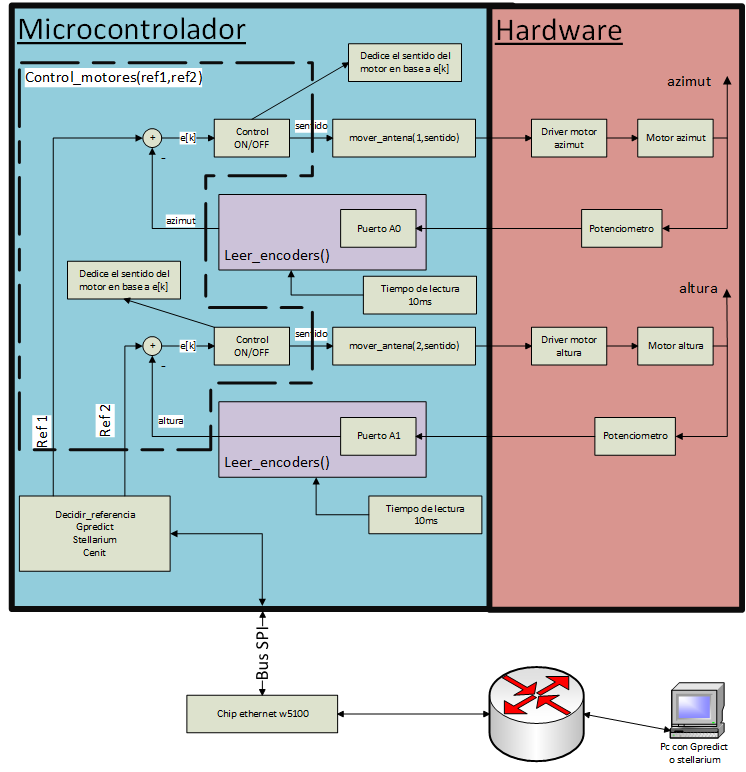
\includegraphics{control_realimentado}
	\caption{Sistema de control microcontrolado implementado en este trabajo.}
	\label{fig:sist_control_real}
\end{figure}

 En base a esta señal de error, que es entrada para el bloque "control ON/OFF", decide hacia donde debe moverse el motor. El sistema se para siempre que la señal de error sea menor que la resolución de cada eje. Este sistema en proximas versiones, se va a cambiar el bloque "controlONOFF" por un controlador denominado PID. 

 El control ON/OFF, actua de según la siguiente tabla, donde para seleccionar el sentido, se basa en las variables movimiento\_motor\_1 y movimiento\_motor\_2, que se obtienen de la función de autocalibración. 
 
 \begin{table}[ht]
 	\centering 
 	\begin{tabular}{|c|c|c|c|}
 		\hline 
 		eje & error & sentido de movimiento & valor variable sentido \\ 
 		\hline	 
 	%	\cline{3-4} 
 		\multirow{3}{*}{Azimut}& $e<-res_{az}$ & este$\rightarrow$ oeste  &movimiento\_motor\_1[1] \\ \cline{2-4}
 		& $e>res_{az}$& oeste$\rightarrow$ este& movimiento\_motor\_1[0] \\ \cline{2-4}
 	%	\hline
 		& $|e|<res_{az}$& motor parado & 0\\ \cline{2-4}
 		\hline   
 		\multirow{3}{*}{altura}& $e<-res_h $ &90° $\rightarrow$ plano del suelo& movimiento\_motor\_2[1] \\ \cline{2-4}
 		& $e>res_h$ &plano del suelo $\rightarrow$ 90° & movimiento\_motor\_2[0] \\ \cline{2-4}
 		& $|e|<res_h$& motor parado& 0\\ 
 		\hline
% 		\cline{2-4}
 		  			
  	\end{tabular}
 \end{table}  
 
 El valor para que se pueda realizar el control correctamente, debe medirse el ruido sobre el sistema(más especificamente, la potencia del ruido),y luego proponer un valor mayor a él para realizar el control, en lugar de la resolución. Se va a probar, si la antena, responde con este valor de resolución, o debe reajustarse. Este procedimiento se realiza al final del presente texto,aclarando dicha situación. El código realizado para el control, se encuentra en el apéndice del presente texto. 

\subsection{Resultados de la función de autocalibración y control}

La función de control, requiere de la definición de los datos brindados por la función de autocalibración. Para la función de autocalibración, en la tabla \ref{tab:result_control} definimos los sentidos, siendo los resultados de las variables los que se encuentran en tabla \ref{tab:resultados_autocalibracion}. Luego, en base a estas variables,se observan cuales puertos son los correspondientes en base a los diodos led referidos en la figura \ref{fig:proto_1}. La resolución, se definió en la sección anterior. El valor de referencia utilizado para realizar las pruebas es el denominado cenit: 90° en altura y 90° en azimut. 

En la tabla \ref{tab:result_control}, se observa que la función de control responde tal cual lo esperado, ya que se observa que al cambiar los puntos iniciales, para el mismo error, se invierte la dirección de los puertos. Esto es así, ya que la función de autocalibración, guarda el sentido de movimiento de la antena, y la función de control, los orienta en el sentido correcto.    


\begin{table}[ht]
%	\hspace{-25mm}
\resizebox{\linewidth}{!}
{
  \begin{threeparttable}		
	\begin{tabular}{|p{1.5cm}|p{1.5cm}|p{1.5cm}|c|c|c|c|c|c|}
		\hline 
		\multicolumn{9}{|c|}{Motor 1: Motor de azimut - Referencia 90º } \\
		\hline 
		\multicolumn{3}{|c|}{autocalibración} & \multicolumn{6}{c|}{control } \\
		\hline 
		\multirow{2}{1.4cm}{Posición inicial} &\multirow{2}{1.4cm}{ Primer Giro} & \multirow{2}{1.4cm}{Segundo giro} &\multicolumn{2}{c|}{$e>res_{az}$} &\multicolumn{2}{c|}{$e<-res_{az}$} &\multicolumn{2}{c|}{$|e|\leq res_{az}$} \\ \cline{4-9}
		
		 & &  & puerto on & puerto off &puerto on & puerto off&puerto off & puerto off\\ 
		\hline 
		punto medio & giro izquierda & giro derecha & MOTOR\_1\_S2 & MOTOR\_1\_S1  & MOTOR\_1\_S1& MOTOR\_1\_S2& MOTOR\_1\_S1 & MOTOR\_1\_S2 \\ 
		\hline 
		punto medio & giro derecha & giro izquierda &MOTOR\_1\_S1  &MOTOR\_1\_S2
		& MOTOR\_1\_S2&  MOTOR\_1\_S1 &MOTOR\_1\_S1 & MOTOR\_1\_S2 	\\
		\hline 
		extremo izquierdo & giro derecha & x &MOTOR\_1\_S2  & MOTOR\_1\_S1  & MOTOR\_1\_S1& MOTOR\_1\_S2 &MOTOR\_1\_S1 & MOTOR\_1\_S2 \\ 
		\hline 
		extremo derecho & giro izquierda & x & MOTOR\_1\_S1&MOTOR\_1\_S2  & MOTOR\_1\_S2 &MOTOR\_1\_S1 &MOTOR\_1\_S1 &MOTOR\_1\_S1  \\ 
		\hline 
		%---------------------------- MOTOR DE ALTURA 	--------------------------%
		\hline 
		\multicolumn{9}{|c|}{Motor 2: Motor de altura - Referencia 90º } \\
		\hline 
		\multicolumn{3}{|c|}{autocalibración} & \multicolumn{6}{c|}{control } \\
		\hline 
		\multirow{2}{1.4cm}{Posición inicial} &\multirow{2}{1.4cm}{ Primer Giro} & \multirow{2}{1.4cm}{Segundo giro} &\multicolumn{2}{c|}{$e>res_h$} & \multicolumn{2}{c|}{$e<-res_h$\tnote{1}}  &\multicolumn{2}{c|}{$|e|\leq res_h$} \\ \cline{4-9}
		
		& &  & puerto on & puerto off &puerto on & puerto off&puerto on & puerto off\\ 
		\hline 
		punto medio & giro izquierda & giro derecha &  MOTOR\_2\_S1 &  MOTOR\_2\_S2  & x & x &MOTOR\_2\_S1 &MOTOR\_2\_S2 \\ 
		\hline 
		punto medio & giro derecha & giro izquierda & MOTOR\_2\_S2 & MOTOR\_2\_S1 & x & x & LOW &LOW \\ 
		\hline  
		extremo izquierdo & giro derecha &x & MOTOR\_2\_S1 & MOTOR\_2\_S2  &   x  & x  &MOTOR\_2\_S1 &MOTOR\_2\_S2 \\ 
		\hline 
		extremo derecho & giro izquierda & x & MOTOR\_2\_S2 & MOTOR\_2\_S1  & x  & x  &MOTOR\_2\_S1 &MOTOR\_2\_S2 \\ 
		\hline 
	\end{tabular}
	\begin{tablenotes}
	 	\small 
	 	\item Los valores de los puertos en on y off,están definidas en el archivo "pinout\_ard\_uno.h", cuyo código se muestra en el código  \ref{cod:pinout_ard_uno.h}.
	 	
	 	\item [1] En el caso del motor de altura, al ser la referencia el máximo valor angular, el error, no puede darse que $e < -res_h $  
	\end{tablenotes}
	\end{threeparttable}
}	
	\caption{Resultados de la funcion de control en conjunto con la función de autocalibración.}
	\label{tab:result_control}
\end{table}


\section{Programación de Scheduler o planificación}

La programación por scheduler(o planificación por su traducción al español), es la base del sistema operativo en tiempo real(ver FreeRtos). El sistema consiste en la ejecución de tareas, que se denominan aplicaciones. Estas tareas, se ejecutan cada cierto tiempo, donde el tiempo lo define el programador. Esto puede definir tareas de mayor o menor prioridad,y permite la ejecución de tareas de forma asincrónica – sincronica. La ejecución sincronica, es la ejecución a tiempo controlado de la aplicación, mientras que la forma asincrónica, puede ejecutarse en cualquier parte del software. En este trabajo, se realiza, la programación de una base de tiempo para controlar la ejecución de tareas, y las funciones necesarias para controlar los relojes. Finalmente se probaron estos relojes, con el uso de un osciloscopio, y midiendo los tiempos.

\subsection{Funcionamiento base de tiempo para scheduler}

Este se basa en el concepto de interrupción.Las interrupciones se explican en el apendice \ref{ap:ard_uno_env}. Se realiza una interrupción por timer. Una interrupción por timer es una interrupción que ocurre con cierta frecuencia,definida por el programador. En el caso del Atmel ATMEGA 328P, posee tres timer, en el presente trabajo, se utiliza el timer2. El diagrama de este se muestra en la figura \ref{fig:timer_2}. 

\begin{figure}[ht]
	\includegraphics{timer_2}
	\caption{Diagrama del timer 2 }
	\label{fig:timer_2}
\end{figure}


Antes de empezar, se debe definir una frecuencia de funcionamiento, para el control del timer. Esta frecuencia se selecciona del clock principal, y se hace pasar por un divisor de frecuencia, llamado preescaler. Este preescaler, solo realiza divisiones de frecuencia en potencias de dos. Este preescaler se configura de un registro llamado “TCCR2B”, que además configura otros parámetros. Una vez configurada la frecuencia de las interrupciones, contamos cuantas interrupciones ocurren, y se tiene el tiempo para cada tarea. 

Este timer tiene 4 modos de funcionamiento. Los cuales son:  

\begin{itemize}
	\item NORMAL MODE 
	\item Clear Timer on Compare Match (CTC) Mode
	\item Fast PWM Mode 
	\item Phase Correct PWM Mode
\end{itemize}

Sin entrar en los detalles de cada uno de ellos, explicados en la hoja de datos del microcontrolador Atmel Atmega328P, los últimos dos modos, se usan para realizar un PWM, y el primero, cuenta hasta una cantidad fija, definida en 255. El modo elegido para este propósito fue el CTC(explicado en la siguiente sección), que es el que mejor se adecua a los requerimientos de una base de tiempo controlada. 

\subsection{Clear Timer on Compare Match (CTC) Mode }

Para configurar este modo, se deben configurar algunos registros, mostrados en la figura \ref{fig:timer_2}. En ella, se ve que los registros, tienen la terminación "nx". Esta terminación corresponde al número de timer y al canal. Así, n puede tomar el valor 0,1 o 2, y x la letra A o B. Por ejemplo el registro OCR2A, corresponde al timer 2, y al canal A del mismo. 
 
El registro TCNT2, se incrementa de a uno, con la frecuencia de preescaler seleccionada en el registo TCCR2B. Cuando el valor de TCNT2 coincide con el valor cargado en el registro OCR2A, se lanza una interrupción por timer. El siguiente esquema aclara lo anterior. 

\begin{figure}[ht]
	\includegraphics{ctc_t2} 
	\caption{Diagrama de tiempos del modo CTC. Extraido de la hoja de datos del microcontrolador}
	\label{fig:ctc_isr}
\end{figure}

En el se ve, que la interrupción se ejecuta cuando TCNT2 alcanza a OCR2A. Para el calculo de la frecuencia, usamos la siguiente formula, que viene dada por el fabricante del dispositivo
\begin{equation} \label{eq:frec_clk_isr2}
	f_{OCnx} = \frac{f_{clk \_ I/O}}{2N(1+OCRnx)}
\end{equation}
donde 

\begin{flalign}
	&f_{OCnx} : \text{frecuencia de el modo CTC.} & \\
	&N : \text{valor del preescaler,son algunas potencias de dos.} & 
	\\
	&f_{clk \_ I/0} : \text{frecuencia del reloj utilizado por el microcontrolador.} & 		
\end{flalign}

Esta ecuación para calcular la frecuencia, es la frecuencia de una onda cuadrada, en el caso de la imagen \ref{fig:ctc_isr}, es el periodo enumerado con "1", en la imagen. Por este motivo, para conocer la frecuencia de la interrupción, se debe multiplicar por dos, al valor que brinda esta ecuación. 


El valor de $f_{clk \_ I/0}$ es 16 Mhz, que es la frecuencia de reloj utilizada por la placa arduino UNO. En este caso, buscamos que el valor sea entero, o múltipo de 10. Para realizar esto, se utilizaron varias pruebas. Se concluyeron los siguientes valores
\begin{itemize}
	\item N = 32
	\item OCR2A = 49
\end{itemize}

Si reemplazamos en la ecuación \ref{eq:frec_clk_isr2} nos brinda un valor de 5Khz. Entonces, la interrupción ocurrira, con una frecuencia de 10Khz, o cada 100 $\mu$s. 

Para configurar el valor de N(denominado preescaler,dentro de la hoja de datos del microcontrolador), y la configuración CTC, dentro de cada timer, existen dos registros de configuración. 
Estos se llamana TCCR2A y TCCR2B, y 
Estos registros se deben configurar con los siguientes valores binarios: 
\begin{itemize}
	\item \textbf{TCCR2A = 0b00000010} 
	\item \textbf{TCCR2B = 0b00000011} 
\end{itemize} 

El valor de cada bit, esta detallado en la hoja de datos del microcontrolador, y no se van a explicar en el presente documento. Al final de realizar todo este analisis, se construyó una función, que automatice esta tarea de configuración. La función tiene por nombre \mintinline{Arduino}{Base_tiempo()}. El código se muestra a continuación. 

\begin{listing}[ht]
	\begin{minted}[linenos,frame=single]{Arduino}
void Base_tiempo()
{
 SREG = (SREG & 0b01111111);
 TCNT2 = 0 ;
 TIMSK2 = TIMSK2 | 0b00000010 ;
 TCCR2A = 0b00000010;
 TCCR2B = 0b00000011; // 0.5 MhZ n= 32 
 OCR2A = 49;
 SREG = (SREG & 0b01111111) | 0b10000000 ;
}	
	\end{minted}
\caption{Función base de tiempo.}
\label{cod:base_tiempo}
\end{listing}

Esta función, además de configurar el modo CTC, el preescalador , y el registro OCR2A, configura las interrupciones. La configuración de las interrupciones puede obtenerse de la hoja de datos del microcontrolador.

\subsection{Programación del Software scheduler} 

El sistema, se compone de una determinada cantidad de relojes, siendo esta cantidad variable por cada programador en la cantidad que se desee. En el caso de este trabajo, se hicieron 8 relojes, y se testearon.
Primero deben crearse los relojes, que pueden o no estar configurados. Estos relojes, los definimos como una matriz de 8x4, donde cada fila es el numero de reloj, y cada columna es hora, minuto, segundo y milisegundo. Esta matriz se llama timer dentro del código. Luego, deben crearse las funciones para interactuar con ella, y además, debe crearse una bandera, que diga, que reloj o relojes se vencieron. Esto se logra con un vector de eventos, donde va guardando los relojes que se vencen. Se usa un vector, porque pueden vencerse mas de un reloj al mismo tiempo. Se lo denomina FlagRepEvent[] . Ademas, creamos un vector que nos indica que relojes están activos, y lo llamamos timer\_activo. Todas estas variables, necesitan, comunicarse entre si, y la comunicación entre ellas se realiza usando funciones. En la figura \ref{fig:soft_sch} se muestra un diagrama del software programado.  


\begin{figure}[ht]
	\includegraphics[width=\linewidth]{software_timer} 
	\caption{Diagrama de software para el software de scheduler}
	\label{fig:soft_sch} 	
\end{figure}

\subsubsection{Funciones}

En primer lugar, se crean dos archivos, uno denominado ``tiempo.cpp''  y ``tiempo.h''. Dentro de ambos archivos se encuentra la programación de las funciones. En el sistema, se crearon las siguientes funciones, las cuales luego se van a encapsular en una librería.  

\begin{itemize}
\item TimerStart(char n\_reloj,char h, char m, char s , int ms)
\item AnalizoTimer(char n\_reloj, char\_index) 
\item timerClose(char n\_reloj) 
\item timerStop(char n\_reloj)
\item timer\_marcha(char n\_reloj) 
\end{itemize}

A continuación se da un breve resumen de lo que realiza cada una de ellas: 

\textbf{TimerStart}:  inicializa el numero de reloj, con la cantidad de tiempo que desea el programador que se ejecute la tarea. Esta función carga la variable timer[n\_reloj][] con los valores de hora, minuto, segundo y milisegundo que desea el programador(es decir, carga la fila), y además carga el vector timer\_activo[] con el valor de reloj. 

\textbf{AnalizoTimer}: Esta función se ejecuta dentro de la interrupción. Su finalidad es descontar un milisegundo a los relojes que previamente se habían cargado. Esta lo que realiza, es solamente el decremento de un milisegundo en los relojes que esten activos en el flag timer\_activo. La función decrementa igual que lo haría un cronometro de bolsillo. Es decir, llega ms a cero, y mira los segundos, si los segundos no son cero, decrementa en uno el segundo, y pone en 999 la variable de ms en el numero de reloj correspondiente.  

\textbf{TimerClose}: Esta función apaga el timer correspondiente, modificando el timer\_activo(poniendolo a cero) y poniendo todo el reloj a cero. 

\textbf{TimerStop}: Deja de contar, es equivalente a parar un cronometro, para luego seguir contando. Esta función modifica timer\_activo y lo pone en cero, pero no modifica el vector de relojes, los cuales siguen sin ser modificados. Para volver a arrancar, se debe utilizar la función timer\_marcha, que vuelve a poner el funcionamiento el reloj que se había frenado. 


\subsubsection{Funcionamiento del software} 

Este software se basa en el concepto de interrupción. Se genera una interrupción cada 100us, y con una variable se cuentan 10 de ellas, y ahí ha transcurrido 1ms. Luego de 10 interrupciones, se llama a la función AnalizoTimer(), que descuenta en un milisegundo de los relojes que esten activos, y si luego de descontar, todo el reloj es cero,(es decir, la fila n\_reloj es toda cero), activa el flagRepEvent correspondiente, para ejecutar la acción correspondiente. Esta acción, es activada por el switch -case de timerEvent() y ejecuta la aplicación correspondiente. 

El modo de utilizarlo es llamar a la función Base\_tiempo(),dentro del inicio del programa, luego con esto, se activan las interrupciones por timer. Acto seguido a esto, hay que definir el numero de reloj a activar con la función TimerStart, o cuando se desee llamar, para activar el reloj correspondiente. Luego, debe definirse la acción a ejecutar por ese reloj, la cual debe estar definida dentro de la función timerEvent. 

Todo el código desarrollado para estas funciones, se encuentra en el anexo del presente capítulo. 



\subsection{Resultados del software de planificación}

Luego de haber construido todo el software, se realizaron pruebas, prendiendo y apagando dos led, cada determinada cantidad de tiempo, y se ha utilizado un osciloscopio para ver la forma de onda.
 
Se configuro un reloj de 872ms, y se midio con un osciloscopio, ambos lanzados a tiempos distintos, es decir, existe un delay entre ambos. Los resultados se midieron en el osciloscopio, en una primera prueba. La segunda prueba, fue configurar dos relojes, y parar uno y relanzarlo, mientras el otro permanecia prendido. Los resultados sobre el osciloscopio se observan en las siguientes imagenes: 


\begin{figure}[ht]
%	\hspace{-20mm}
	\begin{subfigure}{0.5\linewidth}
		\centering
		\includegraphics[width=\linewidth]{osciloscopio_im1} 
		\caption{Primera prueba realizada sobre el software de scheduler}
		\label{fig:osc_m1}	
	\end{subfigure}
	\hfill
%	\hspace{20mm} 
	\begin{subfigure}{0.5\linewidth}
		\centering
		\includegraphics[width=\linewidth]{osciloscopio_im2}
		\caption{Segunda prueba realizada sobre el software de scheduler} 
		\label{fig:osc_m2}		
	\end{subfigure}
	\caption{prueba sobre software de manejo de scheduler}
\end{figure}

Los códigos utilizados para medir esta función, no se encuentra dentro de este documento. Este, debe realizarse utilizando las funciones anteriores, y para la segunda prueba, poner un contador y parar el segundo reloj cuando llegue a un determinado valor, y seguir contando, y cuando alcance un segundo valor,volver a lanzar el mismo reloj. 

Como observamos, en la primer prueba, fue generar una onda cuadrada, donde el estado de alto era de 872ms, y bajo de ese mismo tiempo. En la figura \ref{fig:osc_m1}, se observa la forma de onda en alto, y puede verse que con los cursores del osciloscopio, la medida, fue del mismo tiempo. 

% observaciones imagenes oscioloscopio % 

La segunda prueba, se observa en la imagen \ref{fig:osc_m2}, donde, se ha parado un reloj, durante un tiempo, y se ha vuelto a empezar, manteniendo una onda cuadrada sobre el otro puerto. El resultado fue satisfactorio, ya que se observa, en el osciloscopio, como se ha frenado un puerto, mientras el otro sigue funcionando,y al cabo de un tiempo, volvió a empezar.  
 

\section{Conexión del software con Gpredict y Stellarium} 

En esta sección, se muestran los componentes principales del software desarrollado para comunicarse con estos programas, y como obtener la posición hacia donde debe ir la antena. En la figura \ref{fig:sist_control_real}, se observa un recuadro, que dice "decidir referencia". En esta parte del desarrollo, trata, de ver la forma de decidir esa referencia. Las referencias provienen de tres fuentes posibles: 
\begin{itemize}
	\item Gpredict.  
	\item Stellarium. 
	\item Ninguna - Debe mantenerse en el cenit.
\end{itemize} 

Para ello, dentro del programa principal, se crean dos variables: denominadas \mintinline{Arduino}{ref1} y \mintinline{Arduino}{ref2} respectivamente. Estas tendrán por defecto el valor del cenit (90° en ángulo de azimut y 90° en altura). Cuando existe una conexión, con alguno de estos programas, estos valores cambián automaticamente a aquellas coordenadas enviadas por algúnos de los programas. Una vez finalizada la conexión con alguno de estos programas, estas vuelven a su valor inicial(posición del cenit). 

Antes de empezar a realizar el software para comunicarnos con ambos programas, debe obtenerse la dirección IP, que en esta etapa, será asignada por DHCP. Luego, cuando se conecte a la red institucional, se le asignará una dirección ip fija, dada por el administrador de la red. 

\subsection{Conexión a la red mediante DHCP} 

En principió, el chip ethernet w5100, se conecta a la red, mediante un cable denominado utp. Este cable, se le adiciona un conector, denominado RJ11, en ambos extremos. Este cable, se debe conectar a un router o switch.   

 Una vez, armado el cable y conectado a la red, se debe obtener los parámetros de la red, mediante el uso de el servicio de DHCP(por el momento,en un futuro será fija la dirección IP del dispositivo). El entorno arduino, provee una libreria para trabajar sobre el chip ethernet W5100. Esta libreria, se denomina ``ethernet.h'', y viene por defecto en su entorno. Esta libreria, se provee de varias funciones, para poder realizar la conexión con el chip W5100 y obtener la dirección IP mediante el protocolo DHCP. 
 
 Para comenzar, a utilizar esta libreria, en primer lugar, se debe armar la conexión como muestra la figura \ref{fig:esq_completo}. Una vez armado, se debe conectar el cable de red a la placa que posee el chip W5100. Una vez realizado, se debe realizar la petición DHCP mediante el uso de la libreria. 
 
  
En primera instancia, debe realizarse la configuración del puerto de slave select. Esto se realiza con la sentenca 

\mint{Arduino}|Ethernet.init(PINSS)| 

Una vez definido el pin de chip select, se debe asociar una dirección al dispositivo, denominada ``dirección mac''. Esta dirección es un identificador que esta asociada a cada hardware que desee conectarse a la red. En el caso del chip w5100, esta dirección, se la debe dar el programador, ya que se configura mediante software. La manera de definir una dirección es: 

\mint{Arduino}|  byte mac [] = {0x00, 0xCD, 0xEF, 0xEE, 0xAA, 0xBC};|  

Ahora, debe procederse a obtener la dirección IP por DHCP. Las sentencias para obtener la dirección ip se muestran en el código \ref{cod:dhcpIP}. La dirección IP,que se le asigna mediante el protocolo DHCP, se muestra en el puerto serie, con este código.

\begin{listing}[ht]
	\begin{minted}[linenos,frame=single]{Arduino}
 if (Ethernet.begin(mac) == 0)
{
	Serial.print("obt_Ip") ;
	Serial.print(F("Fallo DHCP"));
	
} else {
	Serial.print(Ethernet.localIP());
}		
	\end{minted}
\caption{Obtención de la dirección IP usando el protocolo DHCP} 	
\label{cod:dhcpIP} 
\end{listing}


Una vez, obtenidos todos los parámetros de la red, se deben configurar los programas, Gpredict, y Stellarium. La dirección IP que se obtuvo a partir de los pasos mencionados, fue la 192.168.0.150. Esta, es la que se va a utilizar para configurar los programas. 

\subsection{Configuración de Gpredict - Programación de la comunicación} 

En primer lugar, debe realizarse la configuración del software Gpredict, siguiendo los pasos que se muestran en la sección \ref{subs:conf_Gpredict}, en la figura \ref{fig:conf_rot_ip}. Antes. de realizar la configuración sobre el software, se debe recordar, que Gpredict, toma el cero del eje azimutal, en el polo norte geografico, y en sentido de las agujas del reloj, aumenta la cantidad de grados, hasta llegar a 360º. Por ende, la configuración de Gpredict en el eje azimutal, debe ser entre 90º(corresponde al este), y 270º(corresponde al
oeste geográfico). Dicho esto, se configura el rotador como muestra la siguiente figura: 
 
\begin{figure}[ht]
	\centering 
	\includegraphics{conf_rotador_gpr}
	\caption{Imagen de la configuración del software Gpredict para la antena ubicada en sala de control del IAR. }
	\label{fig:conf_rot_sala_control}
\end{figure}
%
\subsubsection{Panel de control del rotador}
Si se procede a abrir el rotador recien creado, se observá la siguiente imagén(ver sección \ref{subs:conf_Gpredict}): 

\vspace{20mm}
\begin{figure}[ht]
	\includegraphics{rotador_select}
	\caption{Panel de control del rotador en Gpredict}
	\label{fig:panel_control_gpr}
\end{figure}

Observamos en la imagen, que se tienen los siguientes partes: 

\begin{itemize}	
	\item azimuth: posee las coordenadas del rotador, que se envían mediante el protocolo TCP/IP. Si el rotador esta conectado, en la parte read, aparece la posición del rotador.  
	\item elevación: idem que azimuth, salvo que en el eje de azimuth  
	\item target: Se selecciona el satelite que se desea seguir. Oprimiendo el boton track, se aplica la posición de azimut y elevación del satelite a seguir, tanto a azimuth como a elevación 
	\item settings: Se selecciona el rotador, y en tolerance, indica la tolerancia entre el valor leido y el valor enviado por el rotador. Cycle, es para uso interno del programa, y no debe modificarse. El boton engage es para conectarse al rotador mediante la red.   
\end{itemize}


En la parte izquierda de la figura \ref{fig:panel_control_gpr}, se encuentra una gráfica en coordenadas polares. Los circulos concentricos, indican el ángulo de altura, siendo el circulo exterior un ángulo de altura de 0º, y el centro de 90º. El ángulo desde el norte, en sentido de las agujas del reloj, indica el ángulo de azimuth. Este ángulo es el que esta representado en la ventana de azimuth y elevación, con un circulo rojo. Por ejemplo, en la imagen de la figura \ref{fig:panel_control_gpr}, se observa, 180º azimuth, y 45º elevación,y el circulo rojo, esta marcado apuntando al sur, y aproximadamente en la mitad del radio del centro, hasta el circulo mas grande. La imagen \ref{fig:polar_plot_expl} aclara la explicación dada. En la figura, se observa que hay un recuadro a rayas rojas, esto indica, la visibilidad de la antena instalada en sala de control en el IAR. 


\begin{figure}[ht]
	\centering
	\includegraphics[height=8cm]{polar_plot}
	\caption{Diagrama de gráfico polar en software Gpredict.} 
	\label{fig:polar_plot_expl}
\end{figure}

De la figura, se observa, que en el ángulo de azimuth, se tiene un desfase de 270º, entre la convención de gpredict, y la convención utilizada en este trabajo. Por este motivo, a la coordenada recibida por el software Gpredict, debe restarsele esta cantidad. Si denominamos $\theta_{azgpr}$ a la coordenada recibida por Gpredict, y $\theta_{az}$ a la coordenada que debe apuntarse, según nuestra convención, se tiene la siguiente ecuación :
\begin{equation}
	\theta_{az} =270^\circ - \theta_{azgpr}
\end{equation}

Por último, se observa en la sección target y settings, los botones engage y track. Su comportamiento, se describe con la siguiente tabla: 

\begin{table}[h!]
	\begin{tabular}{|c|c|p{11.0cm}|}
		\hline 
		track & engaje & Descripción. \\
		\hline 
		off & off  & No se envían comandos al rotador y tampoco se lee su posición \\ 
		\hline 
		on  & off  &   La posición del controlador se actualizan con la posición destino pero no se envían comandos al rotador. La posición actual del rotador no se lee. Si el satélite objetivo esta fuera del alcance, las coordenadas del contolador se establecerán en donde se espera que aparezca el satélite. \\
		\hline 
		off & on  &   Las coordenadas azimuth y altura,se envian al rotador, pero no se establece ningún satelite para seguir.  Este modo se puede usarse para controlar manualmente el rotador,o realizar una calibración de la antena. \\ 
		\hline 
		on  & on   &La posición del satelite a seguir, se envia continuamente al rotador en caso de que exista un satelite dentro del campo de visión de la antena. Si el satelite no se encuentra dentro del campo de visión, se establece la ubicación de la antena para esperarlo, y luego seguirlo \\
		\hline 
				
	\end{tabular}
	\caption{comportamiento al oprimir los botones track y engage}
\end{table}

De la tabla anterior, se observa, que la comunicación mediante el protocolo TCP/IP, se debe oprimir el boton Engage. Si se oprime este boton, la coordenada enviada, será la que aparece en la parte del panel donde dice "azimuth y elevación". Si se oprime track, y luego engage, la coordenada enviada por TCP/IP, será aquella en la cual, se encuentre el satelite seleccionado. 

\subsection{Programación del microcontrolador} 

Después de configurar el programa Gpredict, para que realize la comunicación con el dispositivo desarrollado en el presente trabajo, utilizando la libreria ``ethernet'', provista de manera nativa con el entorno de desarrollo arduino, se debe crear un objeto, denominado servidor. La sentencia, para crear este objeto es la siguiente: 

\begin{listing}[ht!]
	\begin{minted}[linenos,frame=single]{Arduino}
#define PORT_GPREDICT 4533 
EthernetServer Gpredict(PORT_GPREDICT)
	\end{minted}

\caption{definición del objeto servidor dentro del entorno arduino}. 
\label{cod:obj_serv_gpr}
\end{listing}
Donde se encuentra definido \mintinline{Arduino}{#define PORT_GPREDICT 4533 }, es el puerto utilizado para la comunicación mediante el protocolo TCP/IP.

Luego, dentro del código principal, se debe realizar una captura de estos datos para poder manipularlos, y responder adecuadamente. Recordar que hay dos tipos de comandos, los comandos de tipo Get y de tipo Set. En la siguiente tabla, se ilustra el formato de los datos, tanto en la respuesta como en la llamada: 
\begin{table}[ht]
	\centering
 \begin{threeparttable}	
	\begin{tabular}{|p{2.0cm}|p{2.0cm}|p{2.0cm}|p{2.0cm}|} 
		\hline
		\multicolumn{2}{|c|}{Comandos tipo Get} &\multicolumn{2}{c|}{Comandos tipo Set}  
		\\ \hline 
		Protocolo de envio & respuesta & protocolo de envio & respuesta \\ \hline 
		comando\tnote{1} & par1$\backslash$npar2$\backslash$n & 
		comando\tnote{1} par1\tnote{2} par2\tnote{2}  $\backslash$n & par1$\backslash$npar2$\backslash$n  \\ 
		\hline 
	\end{tabular}
	\begin{tablenotes}
		\item [1] los comandos estan definidos en la tabla \ref{tab:commands_Gpredict}   
		\item [2] par1 y par2 son las coordenadas de azimut y elevación respectivamente.  
		
	\end{tablenotes}


\end{threeparttable}
	\caption{Envio de respuesta y comandos entre Gpredict y el microcontrolador.}
	\label{tab:protocol_tx_gpr}
\end{table}


Dentro de código principal, para saber si existe algún dispositivo que quiera conectarse, se debe realizar las siguientes sentencias: 

\begin{listing}[ht]
	\begin{minted}[linenos,frame=single]{Arduino}
EthernetClient cliente_gpr = Gpredict.available() ;
if(cliente_gpr)
{

}
	\end{minted}
\caption{captura de paquetes recibidos mediante el software Gpredict}
\label{cod:cliente_gpr}
\end{listing}

Dentro de las llaves iría la acción a realizar según el comando recibido. Los comandos que utiliza Gpredict, son los que se muestran en la tabla \ref{tab:commands_Gpredict}, y el formato para responder a estas peticiones, se encuentran en la tabla \ref{tab:protocol_tx_gpr}.
Para ejemplificar: supongase que se lee el valor de "P 155.20 38.3". Esto significa que debe apuntar la antena al punto 155.20° en azimuth, y 38.3° en altura,pero  debe responder la petición, como indica pa tabla \ref{tab:protocol_tx_gpr}. Si en vez de una P, llegase una "p", este comando, indica que debe responder su posición al programa. Supongamos que la antena, se encuentra en la posición 125.0° en azimut, y 39° en altura, la respuesta a esta petición será "125.0\\n 39°\\n", y en la pantalla de Gpredict, aparecerán estas coordenadas. En este ejemplo, no se aplicó la corrección de las coordenadas,estan implementadas dentro del software. En el caso, que llegue un comando q(desconectarse del gpredict),se debe cambiar la referencia al cenit. En caso de el comando S, se debe para la antena, mediante la función "mover\_antena". 

Todo el código desarrollado se encuentra en el apéndice del presente capítulo. 




\subsection{Stellarium}

Para el stellarium, debe configurarse el software, según la sección \ref{sub:conf_stellarium_red}. Una vez alli, se configura el software como muestra la figura \ref{fig:conf_net_stell}. 

\begin{figure}[ht]
	\centering 
	\includegraphics[scale=0.5]{configuracion_telescopio}
	\caption{configuración del stellarium} 
	\label{fig:conf_net_stell}
\end{figure}  

Una vez configurado, debe presionar "control + 0" o en la barra inferior, debe buscar el icono que le diga "mover el telescopio a las coordenadas definidas. Una vez allí, se le abrirá una ventan con la opción de "configurar telescopio". Debe abrir esa ventana, y le aparecerá el telescopio configurado recientemente. Puede configurar más de un telescopio si así lo desea. Aparecerá una ventana como la que se muestra en la figura \ref{fig:rotador_stellarium_conn}. 
 

\begin{figure}[ht!]
	\centering
	\includegraphics[scale=0.6]{rotador_stellarium} 
	\caption{Apertura del telescopio recién creado.}
	\label{fig:rotador_stellarium_conn}
\end{figure}
Una vez, ahi dentro, presionando el boton conectar, se aprecia la siguiente ventana que aparece en la figura \ref{control del telescopio en stellarium}.  

\begin{figure}[ht!]
	\includegraphics{rotar_telesc}
	\caption{Imagen del panel de control del telescopio usando Stellarium}
	\label{control del telescopio en stellarium}
\end{figure}
donde se observan los siguientes botones y opciones: 
\begin{itemize}
	\item Rotar: envia las coordenadas al dispositivo que mueve la antena, en el caso del presente documento, es el dispositivo desarrollado en este trabajo. 
	\item Sync: En desuso, no posee ningun tipo de uso. 
	\item Ascencion recta: tipo de coordenadas para visualizar estrellas. 
	\item declinación: Idem que ascención recta.  
	\item objeto actual,centro de la pantalla: Permite poner las coordenadas en a donde debe apuntar el telescopio, usando algún astro seleccionado, o el centro de la pantalla. 
	\item HMS, GMS,DECIMAL: tipo de ángulo mostrado. HMS es utilizando el sistema de medición angular basado en horas, el segundo, es el sexagesimal, y el tercero es el decimal. 
\end{itemize}

Este software, no trae límites para el control de la antena, ya que al ser un software utilizado para telescopios, supone que puede girar 360° en azimut y 90° en altura. El sistema de coordenadas utilizado se denomina ecuatorial, y debe realizarse una transformación de coordenadas para poder mover la antena. Esta transformación, se realiza en la siguiente fase del desarrollo del proyecto. 



\subsection{Programación para conectarse con Stellarium}. 

En este caso, se debe definir un nuevo objeto servidor. La nueva definición del objeto se realiza de la siguiente manera: 

\begin{listing}[ht]
	\begin{minted}[linenos,frame=single]{Arduino}
#define PORT_STELLARIUM 10000
EthernetServer stelarium(PORT_STELLARIUM) ;      // socket tcp/ip para stelarium 
	\end{minted}
\caption{definición de objeto servidor para conectarse con el stellarium}. 
\end{listing}

En la sección \ref{sub:comun_stell}, se explica como envía los datos el stellarium, es decir, la trama de datos. En ésta sección, se explica que el programa stellarium, llama a un software externo para enviar estos datos a travez del protocolo TCP/IP. Este se denomina ``telescope\_server''. La codificación que utiliza, es la siguiente, dentro de los bits, la cual según su documentación, utiliza los ángulos en un sistema decimal: 

\begin{itemize}
	\item ascención recta: 
		\begin{itemize}
		 \item	ascención recta 0hs  = 0x100000000 = 		
		 \item	ascención recta 12hs = 0x80000000 
		 \item	ascención recta 24hs = 0x00	
	\end{itemize}
	\item declinación: 
		\begin{itemize}
		  \item	declinacion -90° = -0x40000000
		  \item	declinacion  0°  =  0x00000000
		  \item	declinacion -90° = -0x40000000
		\end{itemize}
\end{itemize}

y con estos valores, se realiza una regla de tres simple, para ambos ejes coordenados. 

Dado que los bits, llegan desordenadados, (es decir, llegan en orden inverso), se los debe ordenar, para luego realizar la regla de tres simple, las instrucciónes para organizar estos datos son: 

\begin{listing}
%\hspace{-30mm}	
\begin{minted}[linenos,frame=single,breaklines]{Arduino}
uint8_t sunP[19] ; 
... 

dec = 0x00000000 | (long (sunP[19])<<24) | (long (sunP[18])<<16) | (long (sunP[17])<<8) | (long (sunP[16])<<0);
RA  = 0x00000000 | (long (sunP[15])<<24) | (long (sunP[14])<<16) | (long (sunP[13])<<8) | (long (sunP[12])<<0);
 	
\end{minted}
\caption{Reorganización de los datos recibidos desde el programa stellarium dentro del microcontrolador}
\label{cod:bitwise_order}
\end{listing}

donde las variables dec y RA, son las coordenadas recibidas desde el software stellarium, los bits recibidos, se guardan en el vector uint8\_t sunP[20].

Una vez se realiza esto, se debe definir el código para que el microcontrolador,se comunique con el software stellarium. Este código, se realiza dentro del bucle principal del programa, y se le añade el código \label{cod:bitwise_order}, dentro del comportamiento. El código es el siguiente: 

\begin{listing}
	\begin{minted}[frame=single,linenos,texcomments,escapeinside=||]{Arduino}
EthernetClient cliente_s = stellarium.available() ; 
long int dec ; 
unsigned long int RA = 0 ; 
uint8_t sunP[20] ; // vector datos recibidos 
char state_con = 0 ; 
if (cliente_s)
{
	% aquí se implementa el código mostrado en| eñ cóigo \ref{cod:bitwise_order}|   
}
	\end{minted}
\caption{Parte del software que se encarga de conectarse con el software stellarium programado dentro del microcontrolador.}
\label{cod:connect_stellarium}
\end{listing} 

Luego, dentro de cada bloque if (ver código \ref{cod:cliente_gpr} y código \ref{cod:connect_stellarium}), van otras lineas adicionales, las cuales no se han mostrado para no extender el documento. Estas lineas adicionales se encuentran dentro del anexo del presente capitulo, y se encargan de mantener la conexión entre los programas de la PC, y el microcontrolador. 
   
\subsection{Resultados de la conexión con Gpredict y Stellarium} 

En esta sección, se comprueba la conexión, el intercambió de mensajes entre stellarium y el microntrolador atmega328p,y el microcontrolador y el Gpredict, utilizando como interface entre la red, el dispositivo el chip ethernet w5100. 

La herramienta seleccionada para realizar este análisis es el software WireShark,que se muestra en el capitulo de redes. Cada software se analiza por separado. Cabe mencionar, que el chip utilizado,no soporta ambos software trabajando en simultaneo, debido a sus limitaciones físicas, impuestas por el fabricante. Por este motivo, se prueban ambos software por separado. 

\subsubsection{Conexión con Gpredict.} 

Una vez, configurado el software Gpredict, para conectarse, se debe abrir el panel de control del rotador, y se debe oprimir el boton ``engage" para calibrar la antena. Si la conexión funciona, dentro de los cuadros de azimuth y elevación, se obtienen las posición de la antena (donde dice ``read'' en la figura \ref{fig:pan_ctrl_antena}). Esta posición, aparece como una cruz roja en el polar plot. El punto rojo, es la posición a la que se debe dirigir la antena, la cual es la coordenada azimuth y altura, marcada con números más grandes en la imagen \ref{fig:pan_ctrl_antena}. 


\begin{figure}[ht]
	\includegraphics[scale=0.7]{gpred_rotador} 
	\caption{Conexión del microcontrolador al software Gpredict mediante el uso del protocolo TCP/IP} 
	\label{fig:prueba_gpredict_1} 
\end{figure}

En la prueba siguiente, se le dió a la antena, una altura de 45° y ángulo de azimuth de 180°. Esta posición esta marcada con un circulo rojo dentro de la gráfica polar. La posición que se encuentra el rotador, es de 253.78° en azimuth y 47.85° en altura, esta posición se encuentra marcada con una cruz roja dentro de la gráfica polar(ver figura \ref{fig:prueba_gpredict_1}). A continuación, se han movido los potenciómetros manualmente,  y se nota que al llegar a la posición, todos los leds del protoboard, permanecen apagados. Esto es un indicativo, que tanto el control como el software responden de manera apropiada. 

 
Luego de esta prueba, se ha probado el seguimiento de un satelite, de forma manual(es decir, moviendo los potenciómetros), en este caso, aparece el circulo rojo, la cruz indicando la posición de la antena, y un punto rojo, el cual indica la posición del satélite en el plano polar. Durante la prueba, se ha utilizado el software wireshark, para monitorizar los comandos enviados y recibidos desde Gpredict. En los comandos enviados y recibidos, no se ha mostrado ningún tipo de anomalia. A continuación se dejan los resultados del panel de control y en la figura \ref{fig:wireshark_gpr} los resultados del análisis hecho con wireshark. 


\begin{figure}[ht]
	\centering
	\includegraphics[scale=0.5]{gpredict_seguimiento_sat} 
	\caption{Panel de control del monitor realizando un seguimiento satelital} 
	
\end{figure}

\begin{figure}[ht]
	\includegraphics[scale=0.5]{wireshark_gpredict} 
	\caption{Captura de paquetes TCP/IP utilizando el programa wirwshark mediante el seguimiento de un satelite} 
	\label{fig:wireshark_gpr}
\end{figure}



\subsubsection{Conexión con Stellarium.} 

En el caso de stellarium, al no poseer un panel de control, como el Gpredict, se debe verificar de alguna forma, que las coordenadas recibidas, sean las correctas. En este caso, se usa el puerto serie como medio de depuración. Dentro del código, se transformán las coordenadas y se verifica que la unidad angular sea la correcta. Además, se realiza una verificación mediante el software wireshark para asegurarse que la comunicación sea fiable, y se respeten los protocolos entre ambos dispositivos(PC y microcontrolador).
Para verificar si las coordenadas son las correctas, se ha oprimido el boton "centro de la pantalla", y luego el boton rotar. La figura \ref{fig:rotador_antena_stell_test} muestra las coordenadas enviadas por el panel de control del telescopio del software stellarium, y en la figura \ref{fig:coord_test_stell} se observan los resultados por puerto serie. 

Cabe destacar, que el ángulo de ascención recta marcado por el stellarium es de -109,41°, y el del programa desarrollado, es de 250.58°. Este desfasaje, se da, por el signo negativo de la ascensión recta. Este signo negativo, indica que es contrario al sentido establecido por los astrónomos en este tipo de coordenadas. Para transformarla, se debe restarle 360° a ese ángulo, y se obtendrá la ascención recta. La cuenta que debe realizarse es: 
\begin{equation*}
	360^\circ - 109.41^\circ = 250.58 
\end{equation*}

 Se observa, que el ángulo coincide, con el valor predichoesto se observa en la imagen \ref{fig:coord_test_stell}.  
\begin{figure}[ht!]
	\includegraphics{rotador_antena_stell} 
	\caption{Panel de control del rotador del stellarium al momento de realizar las pruebas sobre el software} 
	\label{fig:rotador_antena_stell_test}
\end{figure}

\begin{figure}[ht!]
	\includegraphics{puerto_comm_stellarium}
	\caption{Coordenadas recibidas por el stellarium}
	\label{fig:coord_test_stell}
\end{figure}


Además, se revisa la conexión mediante el software wireshark. Los resultados del análisis se muestran a en la imagen 	\ref{fig:wireshark_stell} : 



\begin{figure}[ht!]
	\includegraphics[width=\linewidth]{wireshark_stellarium}
	\caption{Coordenadas recibidas por el stellarium}
	\label{fig:wireshark_stell}
\end{figure}

\section{Unión de partes del software} 

En esta sección se procede a unir todas las partes desarrolladas en esta etapa. Esta unión, se realiza utilizando el esquema de la figura \ref{fig:sistema_general}. La primera parte, debe realizar la función de autocalibración, luego debe iniciar el control de la antena, para volverla a su posición de equilibrio.  

Para realizar el control de la antena, se debe llamar a la función \mintinline{Arduino}{Leer_encoders()}, acto seguido, a la función de control, \mintinline{Arduino}{controlMotores(ref1, ref2)}. Esto debe realizarse periódicamente, por ende, dentro de la programación del scheduler deben ponerse ambas funciones. El tiempo de control seleccionado es 10ms. Estas funciones, se encuentran dentro del archivo "timer.cpp". Para inicializar dichas funciones, se debe realizar el código mostrado en \ref{cod:control_scheduler}. 

\begin{listing}[ht]
	\begin{minted}[linenos,frame=single,escapeinside=||]{Arduino}

#define NUMBER_CLOCK 0 
#define HOUR_CLOCK  0 
#define MINUTE_CLOCK  0 
#define SEGUNDO_CLOCK  0 
#define MILISECOND_CLOCK  10 

|   aqui siguien otras definiciones ... |
...
   |puesta en marcha del control cada 10 milisegundos |
Base_tiempo() ; 
timerStart(NUMBER_CLOCK,HOUR_CLOCK,MINUTE_CLOCK,SEGUNDO_CLOCK,MILISECOND_CLOCK)

| en el bucle principal del programa debe ir |
timerEvent() ; 

	\end{minted}
\caption{inicialización del scheduler para leer los encoders y realizar el control de los motores.} 
\label{cod:control_scheduler}
\end{listing} 

Luego de realizar esto último, se obtiene la dirección IP mediante DHCP , y se programa la conexión dentro del bucle principal del programa. En él código \ref{cod:main_cpp} se muestra la parte de inicialización, y el bucle principal del programa, donde el código obtenido hasta el momento, se muestra en el apéndice del presente capítulo 


\begin{listing}[ht]
	\begin{minted}[linenos,frame=single,escapeinside=||]{Arduino}
void setup() 
{
	// debugger -- 
	Serial.begin(9600) ; 
	/**** inicializacion de puertos del motor como salida  *****/
	init_pins_motores() ; 
	autocalibracion()  ;
	// inicializacion de ethernet 
	Ethernet.init(PINSS) ; 
	byte mac [] = {0x00, 0xCD, 0xEF, 0xEE, 0xAA, 0xBC}; // dirmac
	#if ETHERNET_IP_LOCAL 
	if (Ethernet.begin(mac,ip,DNS,gateway,mask_net) == 0)
	{
		Serial.print(F("Fallo DHCP"));    
	}else 
	{
		Serial.print(Ethernet.localIP());
	}
	#else 
	if (Ethernet.begin(mac) == 0)
	{
		Serial.print(F("Fallo DHCP"));    
	}else 
	{
		Serial.print(Ethernet.localIP());
	}
	#endif
	// inicio scheduler -- > 
	Base_tiempo() ; 
	timerStart(NUMBER_CLOCK,HOUR_CLOCK,MINUTE_CLOCK,SEGUNDO_CLOCK,MILISECOND_CLOCK) ; 
	

}

void loop() 
{
	timerEvent() ; 
	EthernetClient cliente_gpr = Gpredict.available() ;
	EthernetClient cliente_s = stellarium.available() ; 
	long int dec ; 
	unsigned long int RA = 0 ; 
	uint8_t sunP[20] ; // vector datos recibidos -- sunposition 
	char state_con = 0 ; 
	if(cliente_gpr)
	{
		
	} 
	if(cliente_s)
	{
		
	} 
	

}		
	\end{minted}
\caption{código principal del proyecto.}
\label{cod:main_cpp}
\end{listing} 

En esta parte del desarrollo, se ha utilizado el puerto serie para mostrar información.En la próxima sección, se utiliza el display LCD para mostrar información. Esto se realiza en el mismo reloj definido para utilizar la función leer\_encoders y controlMotores(ref1,ref2) ; 

\subsection{Resultados}
Para realizar la depuración del software realizado hasta este momento del desarrollo, se han realizado los siguientes pasos: 
\begin{enumerate}
	\item Se conecto Gpredict con el rotador. 
	\item Se movieron los potenciómetros, y se revisó que el ángulo de movimiento total de la antena sea el de la figura \ref{fig:panel_control_gpr}
	\item Se conecto Stellarium con el rotador.
	\item Se mueve la posición del software stellarium, y quedan registrados los datos por puerto serie.
\end{enumerate}


Luego de realizados estos pasos, se comprobó que todo el software respondia de forma correcta. No se incluira ninguna imagen, ya que las respuestas son las mismas que corresponden a cada sección del presente capítulo de este documento. En esta sección, se ha construido la mayor parte del software. 


\subsection{análisis del código realizado}

En esta sección, se muestran las principales métricas relacionadas al código. 
En primer lugar, se cuentan las lineas de desarrollo, utilizando la herramienta de visual Studio Code denominada VSCodeCounter. Los resultados se resumen a continuación: 
\begin{table}[ht]
	\centering
	\begin{tabular}{|c|c|c|c|c|c|}
		\hline 
		lenguaje& archivos & codigo & comentarios & lineas en blanco & total \\ 
		\hline 
		C++ & 8 &692 &189 &197 & 1078 \\
		\hline 
		ini &1 &13 &9 &2&24\\
		\hline
	\end{tabular}
\caption{Tabla resumén de las lineas de desarrollo realizadas hasta el momento}
\end{table}

Luego de esto, se analiza, los resultados arrojados por el compilador, que el código ocupa 80\% de la memoria de programa, y 52.9\% de la memoria RAM. 

Viendo la gran cantidad de memoria de programa que ocupa, se realizo un análisis con mayor profundidad del código, utilizando una herramienta de desarrollo conocida como ``avr-obj-dump''. La explicación de esta herramienta rebasa el alcance de este documento. Solamente se dirá que es una herramienta para analizar la memoria de microcontroladores AVR, revisando variables, objetos, etc. Una de las conclusiones, que se pueden obtener utilizando esté metodo, es que las librerias de arduino, se cargan de forma completa dentro del microcontrolador. No distingue entre funciones que usa y cuales no, el compilador. Debido a esta situación, se han programado una cantidad moderada de lineas de código para obtener tanta capacidad de memoria flash. A continuación se deja una imagen de los resultados del obj dump 

\begin{figure}[ht]
	\includegraphics{dump_memory}
	\caption{Programa desensamblado en código assembler del microcontrolador. Se utilizó la herramienta avr-obj-dump. }
\end{figure}

\section{Programación del display LCD} 

El entorno arduino, provee una libreria especifica para el manejo del display con el chip pcf8574. Esta se denomina \mintinline{Arduino}{LyquidCrystal\_I2C}. Para utilizarla, se debe incluir en el archivo principal del proyecto. Una vez incluida, se debe crear un objeto LCD, que será el encargado de realizar todas las funciones del display. El objeto LCD se crea de la siguiente forma: 
\mintinline{Arduino}|LiquidCrystal_I2C lcd (ADRRESS\_LCD_I2C,COLS\_LCD,FILAS\_LCD) ; |
Donde ADRESS\_LCD tiene el valor 0x27, que es la dirección del display para el uso del I2C(ver apéndice \ref{AP:protSerial}). 

Algunos de los métodos que posee esta función, son: 
\begin{itemize}
	\item \mintinline{Arduino}{print(String c)}: imprime el String c en el display. 
	\item \mintinline{Arduino}{setCursor(x,y)}: posiciona el cursor en una fila y columna(x es la columna e y es la fila) 
	\item \mintinline{Arduino}{backlight()}:prende el backlight del display LCD.   
\end{itemize}

Estas funciones, serán utilizadas para mostrar información en el display LCD, reemplazando al puerto serie. 


\section{Conclusiones}


En este capítulo, se muestra como han sido los pasos para construir un apuntador de antena basado en tecnología arduino, y sus librerias. Las librerias, poseen la desventaja de cargarse en memoria sin distinción acerca del uso o no de la funcionalidad. Esto, es un punto en contra, pero la velocidad de desarrollo mediante el uso de estas libreria, es superior si uno debe realizar los desarrollos desde cero.  

Se ha logrado realizar un control de tipo ON/Off, a pesar de las limitaciones del microcontrolador, y que respondan de manera adecuada a los requerimientos del proyecto, además, posee un manejo muy preciso de los tiempos de actuación, a pesar de ser un procesador de bajo costo en el mercado local. 


Para finalizar, esta sección, se ha construido la gran parte del software en esta sección, queda la parte de transformación de coordenadas, que será analizada y aplicada en la próxima fase. La construcción de esta función, requiere de conocimientos de trigonometría esférica, ya que todas estas coordenadas utilizadas, se refieren a una esfera. 



\begin{appendices}

	\addcontentsline{toc}{chapter}{anexo capitulo \thechapter}
	\chapter{Códigos de programacion}
	Todos estos códigos, pueden descargarse libremente del repositorio de github, el repositorio es: \url{https://github.com/gaston-cb/control_antena_iar}
	\section{Programación control\_motores} 

	\subsection{Archivo control\_motores.cpp} 


\begin{minted}[frame=single,breaklines,linenos,autogobble=true]{Arduino}
#include <Arduino.h> 
#include "../pinout_ard_uno.h"
#include "../lecturas_encoders/lectura_encoders.h"

#define MOTOR_AZ 1 
#define MOTOR_H 2 

#define PRIMER_SENTIDO_CAL_AZ 1  
#define SEGUNDO_SENTIDO_CAL_AZ 2  
#define PRIMER_SENTIDO_CAL_H 1  
#define SEGUNDO_SENTIDO_CAL_H 2  
#define STOP_MOTOR_1_2 0 

//------------------------ funciones locales en este archivo----------------------------//  

void mover_antena(char _sentido_giro_az, char _sentido_giro_h) ; 
void assign_value_autocal() ; 
void function_compare_autocalibracion() ; 
void assignar_sentidos_motores() ; 


//--------------------------------------------------------------------------------------// 
extern int azimuth ; 
extern int altura ; 


// variables locales al archivo  
int ult4ad[4] ;  // ultimos 4 valores del ad0 y ad1 respectivamente  
/*
* ult4ad[0] = primer_valor_AD_A0   
* ult4ad[1] = segundo_valor_AD_A0
* ult4ad[2] = primer_valor_AD_A1  
* ult4ad[3] = segundo_valor_AD_A1
*/

int calibracion_encoders[4] ; 
/*
* calibracion_encoders[0] : primer valor lectura encoders  -- lectura azimuth  
* calibracion_encoders[1] : segundo valor lectura encoders -- lectura azimuth 
* calibracion_encoders[2] : primer valor lectura encoders  -- lectura altura
* calibracion_encoders[3] : segundo valor lectura encoders -- lectura altura
*/

char estado_autocalibracion[2] = {0,0} ;  // esta variable se usa para scheduler en calibracion  
/*
* estado_autocalibracion[0] --> motor azimuth 
*                           --> 1 ---> primer sentido 
*                           --> 2 ---> segundo sentido 
*                           --> 0 ---> fin calibracion eje azimuth 
* estado_autocalibracion[1] --> motor de altura 
*                           --> 1 ---> primer sentido 
*                           --> 2 ---> segundo sentido 
*                           --> 0 ---> fin calibracion eje azimuth 
* 
* 
*/                           

char movimiento_motor_1[2] ; 
/*
* motor de azimut 
* movimiento_motor_1[0]: sentido  oeste - este 
* movimiento_motor_1[1]: sentido  este  - oeste 
*/
char movimiento_motor_2[2] ; 
/*
* motor de altura 
* movimiento_motor_2[0]: sentido   
* movimiento_motor_2[1]: sentido 
*/

int resH  ; 
int resAz  ; 




enum _state_antena   
{
	AUTOCAL ,  
	NO_AUTOCAL ,  
} antena ; 


struct boolean_ad
{
	unsigned char max_az :1 ;
	unsigned char min_az :1 ; 
	unsigned char min_h  :1 ; 
	unsigned char max_h  :1 ;     
}min_max={0,0,0,0}   ; 


//-------------------------------------------------------------------------------------------//




void init_pins_motores()
{
	pinMode(MOTOR_1_S1,OUTPUT) ; 
	pinMode(MOTOR_1_S2,OUTPUT) ;
	pinMode(MOTOR_2_S1,OUTPUT) ;
	pinMode(MOTOR_2_S2,OUTPUT) ;
}





void autocalibracion()
{
	assign_value_autocal() ;
	delay(1000) ; 
	function_compare_autocalibracion() ; 
	while (estado_autocalibracion[0]!=0 || estado_autocalibracion[1]!= 0)
	{
		delay(1000) ;     
		function_compare_autocalibracion() ;             
	}
	//ASIGNACIÓN DE MOTORES 
	assignar_sentidos_motores() ; 
	antena = NO_AUTOCAL ; 
	#if DEBUG==1
	// depuración por puerto serie . 
	Serial.print("calibracion encoders az: ") ; Serial.print(calibracion_encoders[0]);Serial.print(" ");  Serial.println(calibracion_encoders[1]) ;
	Serial.print("calibracion encoders h: ") ; Serial.print(calibracion_encoders[2]);Serial.print(" "); Serial.println(calibracion_encoders[3]) ;
	Serial.print("movimiento_motor_1: ") ; Serial.print(movimiento_motor_1[0],DEC) ;Serial.print(" ");  Serial.println(movimiento_motor_1[1],DEC) ; 
	Serial.print("movimiento_motor_2: ") ; Serial.print(movimiento_motor_2[0],DEC) ; Serial.print(" "); Serial.print(movimiento_motor_2[1],DEC) ; 
	#endif    
	
}


// n° motor -- sentido -- 
void mover_antena(char n_motor, char sentido_giro)
{
	/*
	*
	*  pines 5 y 6 ---> eje de azimut 
	* _sentido_giro_az =  1 --> pin 5 alto /pin 6 bajo 
	* _sentido_giro_az =  2 --> pin 5 bajo /pin 6 alto  
	* _sentido_giro_az =  0 --> pin 5 bajo /pin 6 bajo 
	* 
	* pines 9 y 10 --> eje de cenith 
	* _sentido_giro_h =  1 --> pin 9 alto /pin 10 bajo 
	* _sentido_giro_h =  2 --> pin 9 bajo /pin 10 alto 
	* _sentido_giro_h =  0 --> pin 9 bajo /pin 10 bajo  
	*  
	*/
	
	if(n_motor == MOTOR_AZ) 
	{
		switch (sentido_giro)
		{
			case 1:
			digitalWrite(MOTOR_1_S1,HIGH) ; 
			digitalWrite(MOTOR_1_S2,LOW) ;
			break;
			case 2: 
			digitalWrite(MOTOR_1_S1,LOW) ; 
			digitalWrite(MOTOR_1_S2,HIGH) ;
			break;
			case 0:
			digitalWrite(MOTOR_1_S1,LOW) ; 
			digitalWrite(MOTOR_1_S2,LOW) ;
			break; 
		}
	}else if(n_motor==MOTOR_H)
	{
		switch (sentido_giro)
		{
			case 1:
			digitalWrite(MOTOR_2_S1,HIGH) ; 
			digitalWrite(MOTOR_2_S2,LOW) ;
			break;
			case 2: 
			digitalWrite(MOTOR_2_S1,LOW) ; 
			digitalWrite(MOTOR_2_S2,HIGH) ;
			break;
			case 0:
			digitalWrite(MOTOR_2_S1,LOW) ; 
			digitalWrite(MOTOR_2_S2,LOW) ;
			break; 
		}
		
	} 
	
	
	
}

void assign_value_autocal()
{
	leer_encoders() ; 
	ult4ad[0] = azimuth ; 
	ult4ad[2] = altura  ; 
	estado_autocalibracion[0] = 1 ; 
	estado_autocalibracion[1] = 1 ; 
	mover_antena(MOTOR_AZ,PRIMER_SENTIDO_CAL_AZ); 
	mover_antena(MOTOR_H,PRIMER_SENTIDO_CAL_H); 
	
}

void function_compare_autocalibracion()
{
	// estado_autocalibracion[] ={ 1,1}  ; 
	leer_encoders() ; 
	ult4ad[1] = azimuth ; 
	ult4ad[3] = altura  ;
	
	
	char flags_status = 'x' ;  
	//motor az ;  motor altura -- flag = 0x33 ambos en estado estacionario 
	//flags que sirven para avisar que se llego a un estado limite dentro de 
	//las comparaciones 
	
	
	// motor de azimut  
	if (ult4ad[1]<100  && min_max.min_az == 0 )
	{
		min_max.min_az = (abs(ult4ad[0]-ult4ad[1])<10)?1:0 ;  
		flags_status = (min_max.min_az==1)?1:'x';  
		
	}else if(ult4ad[1]>800 && min_max.max_az == 0 )
	{
		//min_max.max_az = 1 ; 
		min_max.max_az = (abs(ult4ad[0]-ult4ad[1])<10)?1:0 ; 
		flags_status = (min_max.max_az==1)?1:'x'; 
	} 
	
	
	
	// motor de altura 
	
	if (ult4ad[3]<100 && min_max.min_h == 0)
	{
		min_max.min_h = (abs(ult4ad[3]-ult4ad[2])<10)?1:0 ;  
		if (flags_status==1)
		{
			flags_status = (min_max.min_h==1) ?0x33:1;  
		}else 
		{
			flags_status = (min_max.min_h==1) ?2:'x';  
		}
	}else if(ult4ad[3]>800 && min_max.max_h == 0)
	{
		min_max.max_h = (abs(ult4ad[3]-ult4ad[2])<10)?1:0 ;  
		if (flags_status==1)
		{
			flags_status = (min_max.max_h==1) ?0x33:1;  
		}else 
		{
			flags_status = (min_max.max_h==1) ?2:'x';  
		}        
	}
	
	ult4ad[0] = ult4ad[1] ; 
	ult4ad[2] = ult4ad[3] ; 
	
	switch (flags_status)
	{
		case 1:
		if(estado_autocalibracion[0]==1)
		{
			calibracion_encoders[0] = ult4ad[0] ; 
			estado_autocalibracion[0]=2 ; 
			mover_antena(MOTOR_AZ,SEGUNDO_SENTIDO_CAL_AZ) ;
		}else if(estado_autocalibracion[0]==2) 
		{
			calibracion_encoders[1] = ult4ad[0] ; 
			estado_autocalibracion[0]=0 ; 
			mover_antena(MOTOR_AZ,STOP_MOTOR_1_2) ; 
		}
		break ; 
		case 2:
		if(estado_autocalibracion[1]==1)
		{
			//            Serial.print("est_cal = 1 ") ; 
			calibracion_encoders[2] = ult4ad[2] ; 
			estado_autocalibracion[1] = 2 ; 
			mover_antena(MOTOR_H,SEGUNDO_SENTIDO_CAL_AZ) ; 
		}else if(estado_autocalibracion[1]==2)
		{
			calibracion_encoders[3] = ult4ad[2] ;
			//          Serial.print("est_cal = 2 ") ;
			estado_autocalibracion[1] = 0 ; 
			mover_antena(MOTOR_H,STOP_MOTOR_1_2) ; 
		} 
		break ;
		case 0x33: 
		if (estado_autocalibracion[0]==1 && estado_autocalibracion[1]==1)
		{
			calibracion_encoders[0] = ult4ad[0] ; 
			calibracion_encoders[2] = ult4ad[2] ; 
			estado_autocalibracion[0] = 2 ; 
			estado_autocalibracion[1] = 2 ; 
			mover_antena(MOTOR_AZ,SEGUNDO_SENTIDO_CAL_AZ) ; 
			mover_antena(MOTOR_H,SEGUNDO_SENTIDO_CAL_H)   ; 
			
		}else if(estado_autocalibracion[0]==2 && estado_autocalibracion[1]==2)
		{
			calibracion_encoders[1] = ult4ad[0] ; 
			calibracion_encoders[3] = ult4ad[2] ;     
			estado_autocalibracion[0] = 0 ; 
			estado_autocalibracion[1] = 0 ; 
			mover_antena(MOTOR_AZ,STOP_MOTOR_1_2) ; 
			mover_antena(MOTOR_H,STOP_MOTOR_1_2)   ; 
		}
	} 
	
	
	
} 


void assignar_sentidos_motores()
{
	// motor de azimuth  (cal_enc[0]-->primer sentido )
	/*
	* calibracion_encoders[0] < calibracion_encoders[1] --> sentido = 1 --> sentido este - oeste  
	* calibracion_encoders[0] > calibracion_encoders[1] --> sentido = 1 --> sentido oeste - oeste  
	* 
	*/
	int aux ; 
	#if DEBUG==1
	Serial.println("asig sent motor") ;  
	Serial.print("calibracion encoders az: ") ; Serial.print(calibracion_encoders[0]);Serial.print(" ");  Serial.println(calibracion_encoders[1]) ;
	Serial.print("calibracion encoders h: ") ; Serial.print(calibracion_encoders[2]);Serial.print(" "); Serial.println(calibracion_encoders[3]) ;         
	Serial.println("end assig ") ; 
	#endif
	if(calibracion_encoders[0] < calibracion_encoders[1])
	{
		movimiento_motor_1[0] = SEGUNDO_SENTIDO_CAL_AZ ; 
		movimiento_motor_1[1] = PRIMER_SENTIDO_CAL_AZ;
		
	}else 
	{
		movimiento_motor_1[0] = PRIMER_SENTIDO_CAL_AZ ; 
		movimiento_motor_1[1] = SEGUNDO_SENTIDO_CAL_AZ;
		
		aux = calibracion_encoders[0]   ; 
		calibracion_encoders[0] = calibracion_encoders[1] ; 
		calibracion_encoders[1] = aux ;   
	}
	
	if(calibracion_encoders[2] < calibracion_encoders[3])
	{
		movimiento_motor_2[0] = PRIMER_SENTIDO_CAL_H; 
		movimiento_motor_2[1] = SEGUNDO_SENTIDO_CAL_H; 
	}else 
	{
		
		movimiento_motor_2[1] = PRIMER_SENTIDO_CAL_H; 
		movimiento_motor_2[0] = SEGUNDO_SENTIDO_CAL_H; 
		aux = calibracion_encoders[2]   ; 
		calibracion_encoders[2] = calibracion_encoders[3] ; 
		calibracion_encoders[3] = aux ;   
	}
	resH = abs((100*((90.0)/(calibracion_encoders[2] - calibracion_encoders[3])))); 
	resAz = (100*((180.0 )/(calibracion_encoders[1]- calibracion_encoders[0]))); 
	
	
	
}




void control_motores(int ref_1,int ref_2)
{
	int error_h  = ref_2 - altura ; 
	int error_az = ref_1 - azimuth  ; 
	#if DEBUG == 1 
	Serial.print("resoluciónH: ") ; Serial.println(abs(resH)) ; 
	Serial.print("resoluciónZ: ") ; Serial.println(resAz) ; 
	Serial.print("error alt: ") ; Serial.println(error_h) ; 
	Serial.print("error az: ") ; Serial.println(error_az) ; 
	#endif
	
	// control ON - OFF azimut 
	if(abs(error_az)<resAz)
	{
		mover_antena(MOTOR_AZ,STOP_MOTOR_1_2) ; 
	}else if(error_az>resAz)
	{
		mover_antena(MOTOR_AZ,movimiento_motor_1[0]) ; 
	}else if(error_az<-resAz)
	{
		mover_antena(MOTOR_AZ,movimiento_motor_1[1]) ; 
	} 
	
	// control ON - OFF altura
	
	if(abs(error_h)<resH)
	{
		mover_antena(MOTOR_H,STOP_MOTOR_1_2) ; 
	}else if(error_h>resH)
	{
		mover_antena(MOTOR_H,movimiento_motor_2[0]) ;     
	}else if(error_h<-resH)
	{ 
		mover_antena(MOTOR_H,movimiento_motor_2[1]) ; 
	} 
}

		\end{minted}

	\subsection{Archivo control\_motores.h} 
	

		\begin{minted}[frame=single,breaklines,linenos]{Arduino}
void autocalibracion() ; 
void init_pins_motores() ; 
void control_motores(int ref1,int ref2) ; 
		\end{minted}

	
	
	\section{Programación lectura encoders} 
	\subsection{Archivo lectura\_encoders.cpp} 

		\begin{minted}[frame=single,breaklines,linenos]{Arduino}
#include "Arduino.h" 
#include "../pinout_ard_uno.h"


int azimuth ; 
int altura ;
extern enum _state_antena 
{
	AUTOCAL ,  
	NO_AUTOCAL, 
} antena ;

// variables externas --- Función de autocalibracion  
extern int calibracion_encoders[4] ; 





void leer_encoders()
{
	// int scope_h  ; 
	// int scope_az ; 
	
	int lect_az = analogRead(PINENCODERAZ) ; 
	int lect_h  = analogRead(PINENCODERH) ; 
	if (antena==AUTOCAL) 
	{
		altura = lect_h ; 
		azimuth = lect_az; 
		return  ; 
	}
	// transformación de coordenadas 
	
	altura  = (100*((90.0)/(calibracion_encoders[2] - calibracion_encoders[3]))) *(lect_h - calibracion_encoders[3]) ; 
	azimuth = (100*((180.0 )/(calibracion_encoders[1]- calibracion_encoders[0]))) *(lect_az - calibracion_encoders[0]) ; 
	#if DEBUG==1
	Serial.print("altura: ") ; Serial.println(altura) ; 
	Serial.print("az: ") ; Serial.println(azimuth) ; 
	
	#endif  
	
	
}



		\end{minted}

	
	\subsection{Archivo lectura\_encoders.h} 

	\begin{minted}[frame=single,breaklines,linenos]{Arduino}
	void leer_encoders() ; 
	\end{minted}




	
	\section{Programación del scheduler} 
	\subsection{Archivo tiempo.cpp} 

		\begin{minted}[frame=single,breaklines,linenos]{Arduino}
/*
*   
*   Maquina de timer -
*   Cantidad de relojes - 8 : modificable desde "globales.h". Se debe cambiar #define RELOJES  por el numero deseado
*   Autor : Gaston Valdez 
*   Fecha de prueba : 22/3/2020 - Funciono de manera correcta
*   Prueba - apagado y encendido de leds

*   Nota- Todos estos relojes se suponen bien usados y no hay ningun tipo
*   de check en las funciones. Es deber del programador revisar que no exista
*   ningun fallo de comunicacion entre ellas.

*   No existe comprobacion de TimerStart, POR TANTO DEBE INGRESARSE EL TIEMPO CORRECTAMNETE (ver que ms<1000).
*   Si ms>1000 entonces contara mas de un segundo, la funcion no contaria el tiempo correctamente
*
*   Cada reloj utilizado dentro de TimerEvent() debe cerrarse: hay dos formas distintas
*    1 - poniendo el reloj que se vencio todos sus elementos a cero (es decir TimerStart(n_reloj,0,0,0,0))
*    2 - Usando timerClose(n_reloj)
*    Es importante el cierre de los relojes, ya que ejecutara el case mas de una vez, y el software no es capaz de cambiarlo.
*    
*/

#include <Arduino.h>
#include "../../include/control_motores/control_motores.h"
#include "../../include/lecturas_encoders/lectura_encoders.h"


#define RELOJES 8  
volatile char dec_milis = 0 ;
unsigned int  timer[RELOJES][4]; // vector de relojes
char timer_activo[RELOJES] = {0, 0, 0, 0, 0, 0, 0, 0};
char FlagRepEvent[RELOJES] = {88, 88, 88, 88, 88, 88, 88, 88} ;

extern int ref1 ; 
extern int ref2 ; 




void Base_tiempo()
{
	/*  
	*  Configuracion de registros y flags para habilitar interrupciones
	*  por timer usando timer2 de atmega 328p
	*  Base de tiempo 100 us generacion de interrupcion
	*/
	
	SREG = (SREG & 0b01111111);
	TCNT2 = 0 ;
	TIMSK2 = TIMSK2 | 0b00000010 ;
	TCCR2A = 0b00000010;
	TCCR2B = 0b00000011; // 0.5 MhZ n= 32 
	OCR2A = 49;
	SREG = (SREG & 0b01111111) | 0b10000000 ;
	
}



void TimerStart(char n_reloj, char h, char m, char s, int ms)
{
	/* 
	* Funcion TimerStart:  inicializa y configura un reloj
	*  recibe hora, minutos , segundos y milisegundos para
	*  configurar un reloj dentro de la matriz
	*/
	
	SREG = (SREG & 0b01111111); // deshabilitar int
	char aux = 0 ;
	aux = (timer[n_reloj][0] == 0 && timer[n_reloj][1] == 0  && timer[n_reloj][2] == 0 && timer[n_reloj][3] == 0) ? 1 : 2 ;
	if (aux == 1)
	{
		aux = 0 ;
		// modificar FlagRepEvent
		while (FlagRepEvent[aux] != (n_reloj + 1) && aux < RELOJES - 1)
		{
			aux = aux + 1 ;
		}
		FlagRepEvent[aux] = 88 ;
		
	}
	aux = 0;
	
	
	timer[n_reloj][0] = h  ;
	timer[n_reloj][1] = m  ;
	timer[n_reloj][2] = s ;
	timer[n_reloj][3] = ms  ;
	
	if (ms != 0 || s != 0 || m != 0 || h != 0)
	{
		while (timer_activo[aux] != 0 && aux < RELOJES) {
			aux = aux + 1;
		}
		timer_activo[aux] = n_reloj + 1  ;
	}
	SREG = (SREG & 0b01111111) | 0b10000000 ; // habilitar int
}


void AnalizoTimer(char n_reloj, char index)
{
	/*
	AnalizoTimer - No usada por el usuario
	Funcion invocada por la interrupcion
	Descuenta el tiempo hasta cero y pone un
	flag para generacion de eventos
	
	*/
	timer[n_reloj][3] = (timer[n_reloj][3] != 0) ? timer[n_reloj][3] - 1 : 0 ;
	if (timer[n_reloj][3] == 0)
	{
		if (timer[n_reloj][0] == 0 && timer[n_reloj][1] == 0  && timer[n_reloj][2] == 0) // se vence reloj  -> flagRepEvent[n0_reloj] = reloj + 1 -> N° de reloj (1 a 8)
		{
			FlagRepEvent[index] = n_reloj + 1  ;
			timer_activo[index] = 0 ;
		} else if (timer[n_reloj][2] != 0) // segundos
		{
			timer[n_reloj][2] = timer[n_reloj][2] - 1  ;
			timer[n_reloj][3] = 999 ;
		} else if (timer[n_reloj][1] != 0) // minutos
		{
			timer[n_reloj][1] =  timer[n_reloj][1] - 1  ;
			timer[n_reloj][2] = 59 ;
			timer[n_reloj][3] = 999 ;
		} else if (timer[n_reloj][0] != 0) // horas
		{
			timer[n_reloj][0] =  timer[n_reloj][0] - 1  ;
			timer[n_reloj][1] =  59 ;
			timer[n_reloj][2] = 59 ;
			timer[n_reloj][3] = 999 ;
		}
	}
}




void timerClose(char n_reloj)
{
	/* 
	timerClose() - Usada por el usuario
	Funcion que cierra el numero de reloj
	Pone a cero todo la fila del reloj
	Modifica FlagRepEvent y timer_activo
	*/
	
	SREG = (SREG & 0b01111111); // deshabilitar int
	char aux = TCNT2 ;
	char i = 0 ;
	timer[n_reloj][0] = 0 ;
	timer[n_reloj][1] = 0 ;
	timer[n_reloj][2] = 0 ;
	timer[n_reloj][3] = 0 ;
	
	while (timer_activo[i] != n_reloj + 1 && i < RELOJES - 1)
	{
		i = i + 1  ;
	}
	timer_activo[i] = 0 ;
	
	// ordenar timer activo y cambiar FlagRepEvent
	i = 0 ;
	for (i = 0; i < RELOJES; i++)
	{
		if (FlagRepEvent[i] == n_reloj + 1)
		{
			FlagRepEvent[i] = 88 ;
		}
		if (timer_activo[i] == 0)
		{
			char k = 1 ;
			while (timer_activo[i + k] == 0 && (i + k) < RELOJES)
			{
				k = k + 1 ;
			}
			timer_activo[i] = timer_activo[i + k] ;
			timer_activo[i + k] = 0 ;
		}
	}
	
	TCNT2 = aux ;
	SREG = (SREG & 0b01111111) | 0b10000000 ; // habilitar int
}

void timerCloseAll() 
{
	/*
	* Desactivar todos los relojes activos 
	*/
	char n_reloj = 0 ; 
	for(n_reloj;n_reloj<RELOJES;n_reloj++){
		timer[n_reloj][0] = 0 ;
		timer[n_reloj][1] = 0 ;
		timer[n_reloj][2] = 0 ;
		timer[n_reloj][3] = 0 ;
		FlagRepEvent[n_reloj] = 88 ; 
		timer_activo[n_reloj] = 0 ; 
	}
	
}





void timerStop(char n_reloj)
{
	/*
	Funcion que para el reloj
	Puede seguir contando luego
	Modifica timer_activo y flagrepevent
	Reinicio de reloj - funcion timer_marcha
	La funcion timer_marcha no contempla ninguna validacion de reloj
	Debe ser realizada por el programador y/o modificar este codigo fuente
	*/
	
	SREG = (SREG & 0b01111111); // deshabilitar int
	char i = 0 ;
	// buscar el timer_activo -- desativarlo --
	while (timer_activo[i] != n_reloj + 1 && i < RELOJES  )
	{
		i = i + 1  ;
	}
	timer_activo[i] = 0 ;
	i = 0 ;
	for (i = 0; i < RELOJES; i++)
	{
		if (FlagRepEvent[i] = n_reloj + 1)
		{
			FlagRepEvent[i] = 88 ;
		}
		if (timer_activo[i] == 0)
		{
			char k = 1 ;
			while (timer_activo[i + k] == 0 && (i + k) < 8)
			{
				k = k + 1 ;
			}
			timer_activo[i] = timer_activo[i + k] ;
			timer_activo[i + k ] = 0 ;
		}
	}
	
	SREG = (SREG & 0b01111111) | 0b10000000 ; // habilitar int
}

void timer_marcha(char n_reloj )
{
	/*
	timer_marcha - Usada por usuario
	vuelve a descontar de un contador que se paro.
	con timerStop
	*/
	
	char aux = 0 ;
	while (timer_activo[aux] != 0 && aux < RELOJES )
	{
		aux = aux + 1;
	}
	timer_activo[aux] = n_reloj + 1  ;
	
}



ISR(TIMER2_COMPA_vect)
{
	/*
	Funcion de Interrupcion
	Ocurre cada 100us
	idea - contar 10 interrupciones - > 1 ms
	Reloj con horas - minutos - segundos - milisegundos
	
	*/
	SREG = (SREG & 0b01111111); // deshabilitar int
	char i = 0 ;
	char cant = 0 ;
	dec_milis = dec_milis + 1 ;
	if (dec_milis == 10)
	{
		dec_milis = 0 ;                             //reinicio contador
		while (timer_activo[i] != 0 && i < RELOJES)
		{
			AnalizoTimer(timer_activo[i] - 1, i) ;
			i = i + 1 ;
		}
		/*
		Acomoda el vector timer_activo en caso de algun reloj vencido
		Primeros valores - > relojes activos
		No hay correspondencia entre los relojes y el indice del vector
		*/
		for (cant = 0; cant < RELOJES; cant++)
		{
			if (timer_activo[cant] == 0)
			{
				char k = 1 ;
				while (timer_activo[cant + k] == 0 && (cant + k) < RELOJES)
				{
					k = k + 1 ;
				}
				timer_activo[cant] = timer_activo[cant + k] ;
				timer_activo[cant + k ] = 0 ;
			}
		}
		
	}
	
	SREG = (SREG & 0b01111111) | 0b10000000 ; // habilitar int
	
} // END INTERRUPT



void timerEvent()
{
	/*
	*  Funcion de eventos -
	*  Cuando levanta el flag - inicializa evento segun FlagRepEvent
	*/
	char k ; 
	for (k = 0; k < RELOJES; k++) {
		switch (FlagRepEvent[k])
		{
			case 1:
			leer_encoders() ; 
			control_motores(ref1,ref2) ;  
			break ;
			case 2:
			break ;
			case 3:       
			break ;
			case 4 :          
			break ;         
			case 5: 
			break ;
			case 6 :           
			break ;
			case 7 :            
			break ;
			case 8 :           
			break ;
			default:
			break ;
		}
	}
}
		\end{minted}

	
	\subsection{Archivo tiempo.h} 

		\begin{minted}[frame=single,breaklines,linenos,]{Arduino}
void timerEvent() ; 
void Base_tiempo()  ;
void TimerStart(char n_reloj, char h, char m, char s, int ms) ; 
void AnalizoTimer(char n_reloj, char index) ; 
void timerClose(char n_reloj) ; 
void timerStop(char n_reloj) ; 
void timer_marcha(char n_reloj ) ; 
		\end{minted}

	 
	\section{Archivo principal de programación. main.cpp } 

	\begin{minted}[frame=single,breaklines,linenos]{Arduino}

#include <Arduino.h>
#include "../include/control_motores/control_motores.h"

#include "pinout_ard_uno.h" 
#include "../include/lecturas_encoders/lectura_encoders.h"
#include <Ethernet.h>
#include "tiempo.h"
#include <LiquidCrystal_I2C.h> 
#define ETHERNET_IP_LOCAL 0 //0 -> IP POR DHCP 
#define PORT_GPREDICT 4533 
#define PORT_STELLARIUM 10000
#define NUMBER_CLOCK 0 
#define HOUR_CLOCK  0 
#define MINUTE_CLOCK  0 
#define SEGUNDO_CLOCK  0 
#define MILISECOND_CLOCK  10 




//1 -> ip ASIGNADA POR EL PROGRAMADADOR 
#if ETHERNET_IP_LOCAL      //if  ETHERNET_IP_LOCAL ==1 
byte ip [] = {127,0,0,0}
byte mask_net[] ={127,0,0,0} ; 
byte gateway [] ={127,0,0,0} ; 
byte DNS [] ={127,0,0,0}     ; 
#endif
// prototipo de funciones 
void Asignar_Azimuth_Declinacion(EthernetClient &ptr, String &cad_leida); 
String az_dec_pos_actual();



int ref1 = 9000 ; 
int ref2 = 9000 ; 

EthernetServer stellarium(PORT_STELLARIUM) ;
unsigned long int RA12HS = 0x80000000  ; // 4bytes  
long int DEC10 = 0x40000000  ; //4 bytes 

EthernetServer Gpredict(PORT_GPREDICT) ; 
LiquidCrystal_I2C lcd (ADRRESS_LCD_I2C,COLS_LCD,FILAS_LCD) ; 

// variables externas 
extern int azimuth ; 
extern int altura ;



void setup() 
{	
 // debugger -- 
 Serial.begin(9600) ; 
/**** inicializacion de puertos del motor como salida  *****/
 init_pins_motores() ; 
 autocalibracion()  ;
 //inicializacion de LCD  
 lcd.init() ; 
 lcd.backlight() ; 
 //lcd.print("hola mundillo") ;
	
 // inicializacion de ethernet 
 Ethernet.init(PINSS) ; 
 byte mac [] = {0x00, 0xCD, 0xEF, 0xEE, 0xAA, 0xBC}; // dirmac
#if ETHERNET_IP_LOCAL 
 if (Ethernet.begin(mac,ip,DNS,gateway,mask_net) == 0)
 {
	Serial.print(F("Fallo DHCP"));    
 }else 
 {
   Serial.print(Ethernet.localIP());
 }
#else 
 if (Ethernet.begin(mac) == 0)
 {
   lcd.print(F("Fallo DHCP"));    
 }else 
 {
   lcd.print(Ethernet.localIP());
 }
#endif
 // inicio scheduler -- > 
 Base_tiempo() ; 
 TimerStart(NUMBER_CLOCK,HOUR_CLOCK,MINUTE_CLOCK,SEGUNDO_CLOCK,MILISECOND_CLOCK) ; 
}

void loop() 
{
	timerEvent() ; 
	EthernetClient cliente_gpr = Gpredict.available() ;
	EthernetClient cliente_s = stellarium.available() ; 
	long int dec ; 
	unsigned long int RA = 0 ; 
	uint8_t sunP[20] ; // vector datos recibidos -- sunposition 
	char state_con = 0 ; 
	
	
	
	if (cliente_gpr)
	{ 
		while (cliente_gpr.connected())
		{ 
			timerEvent() ;
			String cadena = "" ;      
			if (cliente_gpr.available())
			{
				//timerEvent() ;  
				char c = cliente_gpr.read()  ;   
				if (c == 'P')
				{
					
					cliente_gpr.print("RPRT 0") ; // lectura correcta 
					Asignar_Azimuth_Declinacion(cliente_gpr,cadena) ;             
					cliente_gpr.flush() ;// VACIADO DE BUFFER 
					cadena ="" ;   
				}else if (c == 'p')
				{      
					cadena = az_dec_pos_actual() ;       
					cliente_gpr.print(cadena);
					cliente_gpr.flush() ; 
					cadena ="" ;     
				}else if (c=='q' || c=='Q' )
				{                
					cliente_gpr.flush() ; 
					cliente_gpr.stop()  ;
					cadena ="" ; 
					break ;          
				}else if (c=='S')
				{
					cliente_gpr.flush() ;  
					cliente_gpr.stop() ;
					cadena = "" ; 
				} 
			}
		}
		cliente_gpr.stop() ; 
		delay(10) ; 
		ref1 = 9000 ; 
		ref2 = 9000 ; 
	}
	
	if (cliente_s)
	{  
		while (cliente_s.connected())
		{
			timerEvent() ; 
			
			char i = 0 ; 
			while (cliente_s.available())
			{
				//Serial.println(cliente_s.read(),HEX) ; 
				sunP[i] = cliente_s.read() ;  
				i = i + 1 ;          
				state_con = 1 ; 
			}
			if(state_con == 1)
			{
				dec = 0x00000000 | (long (sunP[19])<<24) | (long (sunP[18])<<16) | (long (sunP[17])<<8) | (long (sunP[16])<<0);
				RA  = 0x00000000 | (long (sunP[15])<<24) | (long (sunP[14])<<16) | (long (sunP[13])<<8) | (long (sunP[12])<<0);
				state_con = 0 ; 
				// declinacion en angulo 
				//ra en angulo 
				// RA12HS -- 12hs 
				unsigned long int hsra = (((RA*12.0)/RA12HS) * 10000)*15   ;
				float hsrf  = ((RA*12.0)/RA12HS)*15 ;      
				float declinacion = (90.0/DEC10)*dec ;  
				
				Serial.print("declinacion: ") ; Serial.println(declinacion) ; 
				Serial.print("ascencion recta: ") ; Serial.println(hsrf) ; 
				Serial.print("ascencion recta entera: ") ; Serial.println(hsra) ; 
				cliente_s.write(sunP,20) ;   
			}
			
		}
		cliente_s.stop() ; 
		delay(10) ; 
		// change ref1 and ref2  in future part of the project 
	}

}




void Asignar_Azimuth_Declinacion(EthernetClient &ptr, String &cad_leida)
{
	/*
	* Esta funcion esta destinada a recoger los datos del 
	* Gpredict y guardarlos en una variable para poder 
	* global para poder compararlos. Se realiza una conversion a valor 
	* entero y se comparan entre ellos para obtener la posicion actual. Si son 
	* coincidentes se detiene el motor, si no, se gira a la derecha o izquierda segun 
	* el caso
	* 
	*/
	float az = 0  ;
	float alt = 0  ;
	ptr.read(); //espacio en blanco  
	while(ptr.available())
	{ 
		char c = ptr.read() ; 
		cad_leida+= c==','?'.':c;   
	}
	
	
	az = (cad_leida.substring(0,cad_leida.indexOf(' '))).toFloat();
	alt = (cad_leida.substring(cad_leida.indexOf(' '))).toFloat(); 
	
	//conversion a valor entero 
	ref1 =  27000 - (az*100) ; 
	ref2 =  (alt*100) ;  
	
	
}


String az_dec_pos_actual()
{
	Serial.print("azimuth: "); Serial.println(azimuth) ; 
	
	return String(String(270.00 - azimuth/100.0) +'\n'+String(altura/100.0))+'\n' ; 
}

		\end{minted}

	 
	
\end{appendices}
	


%-----------fin segunda fase---------------------% 

% tercera fase 
\part{Física de los satelites y sistemas de coordenadas astronómicas}
%\renewcommand{\chaptername}{Dinámica de los satelites  elementos keplerianos}
\chapter{Dinámica de los satelites  elementos keplerianos}
\markright{Dinámica de los satelites  elementos keplerianos}
\section{Introducción} 
En este capítulo, se introducen los conceptos básicos relacionados con la física de los satelites, cálculo de las orbitas, y su solución para encontrar las posiciones de los satelites. Estas posiciones vienen dadas desde una base de datos, pero el software (gpredict ystellarium), deben calcular las posiciones en base a su última actualización. La materia que se encarga de este estudio, se denomina mecánica órbital. Esta materia, es absolutamente general, ya sea para movimientos de estrellas, satelites naturales y artificiales. Sus principios son dos leyes básicas de la naturaleza: Las tres leyes de newton y las tres leyes de keepler. A partir de estas dos leyes, y utilizando calculo diferencial, puede obtenerse la solución, para las posiciones de los satelites,estrellas,etc, en función del tiempo, a partir de una condición inicial. 


\section{Conceptos básicos}

En esta sección, se abordan los conceptos básicos para la deducción de las tres leyes de kepler. Se omiten los conceptos de cálculo diferencial y vectores en el plano.Si el lector no esta familiarizado con algunos de estos temas, se sugiere revisar literatura al respecto. Además, si el lector, esta familiarizado con las leyes de newton, sistemas de coordenadas, puede saltearse esta sección. 


Para una compresión completa de la mecánica de los objetos celestes(ya sea satelites artificiales, naturales, y estrellas,etc), se requiere en primer lugar un sistema de coordenadas,y un sistema de referencia de tiempo. En general se elige el centro del sistema de coordenadas, como el centro del planeta tierra, ya que la mayor parte de las observaciones se realizan desde la tierra.

\subsection{cinemática}
	Para seguir el movimiento de una particula en el espacio euclideo,se necesita un marco de referencia, que consta de un reloj, y un sistema de coordenadas. En mecanica no relativista, el reloj es universal para todos los sistemas de coordenadas. Dada una particula P, que esta en un instante t, en la posicion $r(t)$ dada por: 
	$r(t)=x(t)i + y(t)j +z(t) k $ 
	 


% vectores 
% conceptos básicos de leyes de newton 
% fuerza coriolis y deducción de la aceleración en mecanica analítica 
% sistemas de referencia 
% derivada del vector rotacion angular 
% leyes de gravitación universal 
\section{Leyes de kepler}
\subsection{Problema de los dos cuerpos}
\subsection{Problema de n cuerpos} 
\section{Parámetros orbitales o keplerianos}
\section{Determinación de las orbitas} 

\section{Involucrando el tiempo en las ecuaciones} 
\section{Calculos de orbitas y modelos matematicos}
\section{estaciones terrenas}
\renewcommand{\chaptername}{Sistemas de coordenadas astronómicas}
\chapter{Sistemas de coordenadas astronómicas} \label{cap:sist_cord} 
\markright{Sistemas de coordenadas astronómicas} 
\begin{center}
	\begin{tcolorbox}[colback=gray!5!white, %Color del fondo
		colframe=blue!75!black,
		title= \center{\Large{Resumen}} ]
	Se explican, los fundamentos de las coordenadas astronómicas. Además, se explican algunos de los sistemas de coordenadas utilizados en astronomía. Esta descripción es necesaria, para poder realizar la transformación de coordenadas dentro del microcontrolador, en caso que se este siguiendo una estrella o satélite,mediante el programa Stellarium,
	\end{tcolorbox}
\end{center}    

\section{introducción} 

En este capítulo se describe como realizar la transformación de coordenadas. El microcontrolador, recibe las coordenadas en coordenadas ecuatoriales horarias(con el software Stellarium), y debe realizar la transformación de coordenadas a ecuatoriales locales, luego debe realizarse otra transformación, al sistema horizontal local, dado el tipo de montura(altazimutal) que posee la antena. El presente texto, intenta explicar cuáles son los sistemas de coordenadas usados en astronomía, y necesarios para el presente trabajo. Existen más sistemas de coordenadas, pero rebasan el alcance del proyecto, el lector interesado puede ver la referencia \cite{Baume2014}. Para ello, se debe empezar conociendo conceptos básicos de la trigonometría esférica, esfera celeste, etc. Al lector que este familiarizado con estos temas, puede omitir este capítulo. 

\section{Esfera - Elementos fundamentales} 


La superficie más usada a lo largo del presente capítulo es la esfera. Por este motivo, se va a definir una esfera, en conjunto con sus elementos fundamentales. A partir de esto, obtendremos algunos resultados de una materia denominada trigonometría esférica. Esta, se plantea en la superficie de una esfera, a partir de los elementos básicos de ella, por ello, el concepto de esfera y sus elementos es importante para comprender el resto del capítulo. Cabe recordar, que una esfera también puede escribirse en coordenadas esféricas.  

  
Definición de esfera[1] Conjunto de puntos del espacio equidistantes de otro punto fijo. 
Sobre esta definición, al punto fijo, se lo conoce como centro de la esfera y lo vamos a denotar con la letra O. La distancia desde O a cualquier punto, se denomina radio de la esfera (R)  
Si a la esfera, le hacemos pasar un plano, según este plano contenga a O, o no, podemos definir dos tipos de círculos o circunferencias: 
\begin{itemize}
\item Circunferencia máxima (o circulo máximo): Circunferencia que se obtiene al cortar la esfera con el plano que contiene a O 
\item Circunferencia menor (o circulo menor): Si el centro de la esfera(O) no esta contenida en el plano que corta a la esfera. 
\end{itemize}

Ahora, para definir las posiciones de un punto, sobre la esfera, es necesario definir círculos de referencia, usando círculos menores y mayores. Si se tiene un círculo máximo, y se traza una recta perpendicular al plano del circulo máximo, y que pase por O, esta recta, corta a la esfera en dos puntos, denominados polos. Además de estos elementos, se tienen los siguientes: 


% cuarta fase 
\part{Sistema electrónico de posicionamiento - Construcción de prototipo y resultados}

%\backmatter 
%apendices 
\renewcommand{\appendixname}{Apéndice}
\renewcommand{\appendixtocname}{Apéndice}
\renewcommand{\appendixpagename}{Apéndice}



\appendix
\clearpage
\addappheadtotoc
\appendixpage
\appendixtitletocon
\renewcommand{\chaptername}{Protocolos de comunicación Serie}
%\graphicspath{{Apéndice/ComSPII2C/}}
\chapter{Protocolos de comunicación Serie}\label{AP:protSerial}
\section{Introducción}
En la presente sección, se describen dos protocolos utilizados con los periféricos seleccionados para el presente trabajo final. Los dos protocolos que utilizan estos dispositivos se denominan Serial Peripherical Interface o SPI, por sus siglas en inglés, y el protocolo I2C (también se lo puede encontrar con el nombre de Two Wire o TWI). Ambos protocolos definen señales de entrada y salida, y un dispositivo maestro, que es el encargado de enviar los datos a los periféricos correspondientes. En este trabajo, el dispositivo maestro, es el microcontrolador ATmega328P. Ambos protocolos son de tipo serie. Además, se revisa el pinout disponible de cada dispositivo, y se da una breve explicación sobre cada pin que poseen los perifericos(w5100 ethernet y display LCD con chip adaptador para I2C. 


\section{Protocolo SPI}

El protocolo SPI, define tres señales: MOSI,MISO y SCK o CLOCK. Dado que el protocolo SPI,consta de un dispositivo maestro, puede constar de varios dispositivos esclavos. Para seleccionar el dispositivo con el que se quiere comunicar, se debe agregar un cable adicional por dispositivo, este cable adicional se denomina Slave Select, o SS. El dispositivo maestro, selecciona un dispositivo esclavo para comunicarse a traves de esta linea, denominada SS. A continuación se deja una imagén de las conexiones entre un dispositivo maestro y tres esclavos: 

\begin{figure}[H]
	\centering	
	\includegraphics{Apéndice/ComSPII2C/SPIconn.png}
	\caption{Esquema de conexiones entre un dispositivo maestro y un dispositivo esclavo usando el protocolo SPI.}
	\label{fig:master_slave_SPI}
\end{figure}

Las señales que utiliza el protocolo SPI son las siguientes: 
\begin{itemize}
	\item SCK o CLOCK: Se encarga de generar una señal de reloj. Esta señal es generada por el dispositivo maestro.
	\item MOSI(Master Output Slave Input): Son los datos que envia el dispositivo maestro al esclavo. 
	\item MISO(Master Input Slave Output): Son los datos que envia el dispositivo esclavo al maestro. 
\end{itemize}

El dispositivo maestro, es el encargado de seleccionar a que dispositivo se quiere comunicar, mediante la linea o cable de SS en la figura \ref{fig:master_slave_SPI}. Además, el maestro, puede recibir información del dispositivo esclavo. Por tanto, la comunicación es de tipo "Full Duplex"(ambos dispositivos son capaces de transmitir y de recibir al mismo tiempo). Todos los datos salientes, se transmiten en serie, por ende, es requisito, que cada disposivo maestro y/o esclavo, posean un registro de desplazamiento a medida que se reciben los datos.     
 
Esta comunicación es sincrónica, la señal de CLOCK, genera una señal de reloj,de una determinada frecuencia, y esta es utilizada para la sincronia con las señales MOSI y MISO respectivamente, para que se transfieran los datos entre si. La señal de clock, solo esta activa durante la comunicación, luego se queda en estado alto o bajo, según se haya definido previamente. Debido a esto, se pueden definir cuatro modos de funcionamiento, dos basados en la polaridad del reloj, y otros dos, basados en la fase de la señal de reloj. A continuación se deja un diagrama de tiempos de las señales involucradas en el protocolo SPI.  

\begin{figure}[ht]
	\includegraphics[width=\linewidth,height=8cm]{Apéndice/ComSPII2C/SPI_timing.png}
	\caption{Señales del protocolo SPI en función del tiempo.La letra z dentro del diagrama indica estado de alta impedancia}
	\label{fig:señales_SPI}
\end{figure}

Como se observa, en la figura,primero se pone la señal de slave select(ss) en nivel bajo, y luego empieza la comunicación. Cuando finaliza la comunicación, vuelve a su estado alto.Las señales se denominan CPOL por las siglas de "clock polarity" y CPHA por "clock phase". De la figura, se observa que hay cuatro modos de funcionamiento: 

\begin{itemize}
	\item Modo 0: Con CPOL = 0 y CPHA = 0. Modo en el cual el estado del reloj permanece en estado lógico bajo y la información se envía en cada transición de bajo a alto, es decir alto activo.
	\item Modo 1:CPOL=1 y CPHA = 1. El estado del lógico del reloj es alto, y se envian datos cuando hay una transisción del estado alto al estado bajo. 
	\item Modo 2: CPOL = 1 y CPHA =0. El estado lógico del reloj es alto, y se envian los datos, y se envian en cada transicion de bajo a alto.(existe un desfase entre el estado logico y el envio de los datos).   
	\item Modo 3: CPOL = 1 y CPHA = 1. Modo en el cual el estado del reloj permanece en estado lógico alto y la información se envía en cada transición de alto a bajo, es decir bajo activo.(existe un desfase entre el estado logico y el envio de los datos). 
\end{itemize}

Por ultimo, se debe destacar, que no todos los dispositivos soportan todos los modos, por ende, para realizar una comunicación entre dos dispositivos, se debe verificar que ambos por los menos tengan un modo en común para que la comunicación pueda llevarse a cabo. 



\section{Procotolo I2C}

El protocolo I2C, o Wire Serial, es un protocolo de comunicación serie, el cual define dos señales: SDA y SCL.La señal SDA es para transmitir los datos en formato serie(SDA proviene de las siglas serial data), y SCL, es una señal de reloj(SCL proviene de serial clock, en otras bibliografias, las puede encontrar como SCK o CLK). 

Este protocolo, presenta una arquitectura del tipo maestro esclavo. El maestro es el encargado de enviar los datos, y los reciben los esclavos. Puede existir más de un maestro. El diagrama eléctrico es el siguiente: 

\begin{figure}[ht]
	\includegraphics[scale=0.8]{Apéndice/ComSPII2C/busI2C.png}
	\caption{diagrama de las conexiones entre una maestro y n esclavos mediante el uso de el protocolo I2C} 
	\label{fig:busI2C}
\end{figure}

Dado, que solo tiene dos cables, la forma de identificar un dispositivo es mediante una dirección, esta dirección, es un número binario formado por 7 bits, o 10 bits(en este último caso, son muy escasos los dispositivos), según el dispositivo. Si la dirección del esclavo, contienen solo 7 bits, esto quiere decir, que se puede conectar hasta 128 dispositivos. Esta dirección, debe ser dada por el fabricante del dispositivo o debe configurarse de alguna forma provista por el fabricante.  

El maestro, se comunica con los esclavos, mediante el uso de una secuencia de inicio, y una secuencia de parada, con esto, los esclavos reconocen si se quiere comunicar con alguno de ellos. Entre mensajes, existen bits de reconocimiento que el esclavo envía al maestro, para que el maestro pueda reconocer de que forma se estan recibiendo los datos por parte de los esclavos o esclavo correspondiente. 

\begin{figure}[ht]
	\includegraphics[scale=0.5]{Apéndice/ComSPII2C/timing_I2C.png}
	\caption{Diagrama de tiempos que utiliza el protocolo I2C.En este caso, seutiliza una dirección de 7 bits}
	\label{fig:timing_I2C}
\end{figure}

Como se observa en la figura \ref{fig:busI2C}, el estado del canal de comunicación por defecto es el estado alto. Cuando el master quiere iniciar la comunicación, pone la linea SDA en bajo,eso le indica a los esclavos que se va a iniciar una comunicación por parte del master. Acto seguido, se inicia la señal de SCL, la cual es una señal de reloj(ver figura \ref{fig:timing_I2C}). Luego se envian de forma sincronizada la dirección del esclavo con el cual se quiere comunicar, y un bit extra, el cual le avisa si requiere información del dispositivo o va a enviarle información. El dispositivo que posee esa dirección, reconoce que le van a enviar datos, y envia un bit de ACK, sobre la linea SDA, poniendola en bajo. Luego, envia otros 8 bits, y el esclavo envia un ACK, ponieno la linea SDA en bajo. Asi, cada 8 bits, luego cuando la linea SCL permanece en alto, significa que la comunicación ha finalizado. Si el dispositivo no esta disponible, o no existe esa dirección, la señal SDA permanece en alto, y se corta la comunicación.Por otro lado, si la comunicación es del esclavo al maestro, el maestro tambien debe enviarle el bit de confirmación correspondiente.  

Cabe destacar, que la velocidad de comunicación viene dada por la señal de reloj. Se definen cuatro modos de velocidad para el bus I2C: 
\begin{itemize}
	\item MODO ESTANDAR
	\item MODO RAPIDO 
	\item MODO HIGH SPEED
	\item MODO ULTRA FAST 
\end{itemize}

Cada modo, define una frecuencia para su señal de reloj. Cuando se desean conectar maestros y esclavos, debe verificarse con su hoja de datos que ambos posean el mismo modo de velocidad, para cada dispositivo. 


\section{Chip ETHERNET W5100 shield }

El chip ethernet W5100, ya viene en un módulo integrado, mostrado en la figura \ref{fig:chip_ethernet}. Este módulo, posee 10 pines. Este módulo, trae un circuito integrado denominado W5100, el cual, se utiliza para proveer soluciones ethernet. Soporta los protocolos TCP/IP, y se puede configurar, para que se conecte a la red local mediante un cable ethernet. 

Los puertos que tiene este módulo son los siguientes(ver figura \ref{fig:ap_ethernet}):

\begin{itemize}
	\item pin Vcc: Pin donde se debe conectar una fuente de alimentación de 5Volts
	\item pin GND: Se conecta la tierra del sistema. 
	\item pin SS: Cable de slave select para el protocolo SPI 
	\item pin MOSI:Linea MOSI para el protocolo SPI  
	\item pin MISO Linea MISO para el protocolo SPI  
	\item pin SCK o CLOCK: Linea CLOCK para el protocolo SPI  
	\item pin Reset: Resetea el dispositivo ethernet, borrando todas sus configuraciones. 
	\item pin P+: Power of Ethernet. Cable destinado a recibir alimentación por la linea de red ethernet.Recibe potencia positiva 
	\item pin P+: Power of Ethernet. Cable destinado a recibir alimentación por la linea de red ethernet.Recibe potencia negativa  
\end{itemize}

Cabe destacar, que las lineas P+ y P-, son para poder utilizar el estandar "Power of Ethernet", el cual define lineas para la transmisión de la alimentación a traves de un cable de red. 

\begin{figure}[ht]
	\centering 
	\includegraphics{parte_2/soft_micro/pinoutW5100}
	\caption{Esquema de pines que posee el modulo W5100.} 
	\label{fig:ap_ethernet}
\end{figure}

Si se observa la hoja de datos del dispositivo, se observan que los modos SPI soportados son los modos 0 y 3 respectivamente. 


\section{Display LCD con adaptador para I2C }

En el caso del display, el display, trae integrado un adaptador para I2C. Este adaptador es el circuito integrado PCF8574. Este según su hoja de datos, se utiliza para expandir la cantidad de puertos de un microcontrolador, mediante el protocolo I2C a través de dos puertos, ya que este protocolo solo utiliza dos lineas para su comunicación. 

Este dispositivo, (PCF8574) puede usarse para leer los puertos a la salida, o para escribir los puertos a su salida. En este caso particular, esta placa con este circuito integrado, esta realizada para aplicarla exclusivamente a los display LCD, y se provee la libreria para su uso con el display LCD. 

Para conocer la dirección de comunicación, se debe revisar la hoja de datos, y puede darse hasta 8 direcciones distintas, en base a los puertos del circuito integrado, denominados A0,A1,A2,por el fabricante. Estos puertos del circuito integrado PCF8574 se encuentran disponibles en la placa para ser modificados. La siguiente imagen muestra su ubicación en la placa: 

\begin{figure}[ht]
	\includegraphics[scale=0.8]{Apéndice/ComSPII2C/display_LCDATRAS}
	\caption{Foto del display LCD de la parte de atras, donde se observan los pines A0,A1 y A2 accesibles para poder modificarlos.}
	\label{fig:pcf8574_LCD} 
\end{figure}

Esta placa por defecto, trae todos los pines A0,A1 yA2 en alto. Si queremos pasar algun de esos puertos a bajo, se debe estaniar en donde se encuentra el cuadrado rojo en la imagen \ref{fig:pcf8574_LCD}. De la hoja de datos, se explica que la dirección posee 7 bits, donde los siete bits estan dados por la forma 0100A2A1A0, si A0,A1 o A2 esta en alto, se indica un uno, caso contrario, se completa con cero. Por ejemplo si consideramos el caso de la figura, no ha sido modificado, por ende, A2 = 1 , A1 = 1 y A0 = 1. Esto nos indica que el dispositivo tiene la dirección 0100111, que es 27 en base hexadecimal. 

Entonces, este procedimiento de poder cambiar la dirección del puerto I2C, permite conectar hasta 8 chips iguales, obteniendo 64 puertos de entrada y salida, manejado unicamente desde un dispositivo maestro, a través de dos lineas. Esto claramente presenta la ventaja de requerir menor cantidad de puertos, que un display LCD, y la diferencia de precios entre un display LCD, con chip I2C es infima, y no conviene optar por el display LCD sin el chip(la diferencia en pesos argentinos ronda los \$200,en esta epoca equivale a un 1,25 dolares aproximadamente). 

Los puertos que tiene disponibles a la salida, son Vcc Y GND. En el pin de Vcc deben conectarse 5 volts, y en GND la tierra. Los puertos SDA y SCL, son los puertos del protocolo I2C, y se deben conectar como en la figura \ref{fig:busI2C}. En el caso, de conectarla a la placa Arduino Uno, como en este caso, las resistencias de pull-up, estan implementadas sobre la misma placa. 






\chapter{Programación sobre plataforma Arduino UNO - Periféricos del microcontrolador} \label{ap:ard_uno_env}
\section{PlatformIO - Configuración y flags de compilación}
\section{Primer Programa}
\section{Compilación condicional}
\section{Sentencias sobre el entorno arduino}
\section{Conversor Analógico Digital}
%bibliografia  

%	
\backmatter 
\printbibliography[heading=bibintoc,
				   title=bibliografía,
				  ]	
	\nocite{*}
\end{document}




